\documentclass[12pt]{book}

\usepackage{hyperref}
\def\chapterautorefname{Chapter}
\def\sectionautorefname{Section}
\def\subsectionautorefname{Section}
\def\subsubsectionautorefname{Section}

\usepackage{algorithm}
\usepackage{algpseudocode}
\algrenewcommand\algorithmicrequire{\textbf{Input:}}
\algrenewcommand\algorithmicensure{\textbf{Output:}}
\algnewcommand\Not{\textbf{not} }
\newcommand{\algorithmautorefname}{Algorithm} % autoref

\usepackage{adjustbox}
\usepackage[headings]{fullpage}
\usepackage{xargs}
\usepackage{xspace}
\usepackage[doublespacing]{setspace}

\usepackage{microtype}
\usepackage[T1]{fontenc}

\usepackage{wrapfig}
\usepackage[font={sf}]{caption}
\usepackage[subrefformat=parens]{subcaption}

\usepackage{multirow}

\usepackage{xcolor}
\usepackage{graphicx}
\graphicspath{{_build/}{figures/}}

\usepackage{amsmath}
\newtheorem{definition}{Definition}[chapter]
\newtheorem{theorem}{Theorem}[chapter]
\newtheorem{proof}{Proof}[chapter]

\setlength{\marginparwidth}{2cm}
\usepackage[textsize=tiny]{todonotes}
\renewcommand\max[2][]{\todo[color=orange, #1]{\sffamily #2}}

\usepackage{libertine}
\usepackage[libertine]{newtxmath}
\usepackage[scaled=.85]{DejaVuSansMono}

\usepackage{listings}
\lstset{
  columns=fullflexible,
  keepspaces=true,
  showstringspaces=false,
  stringstyle=\slshape\color{green!40!black},
  basicstyle=\ttfamily\small,
  language=Python,
  morekeywords={*, self},
  commentstyle=\slshape\color{black!60},
  tabsize=2,
}

\lstdefinelanguage{Rust}{
  sensitive,
  morecomment=[l]{//},
  morecomment=[s]{/*}{*/},
  moredelim=[s][{\itshape\color[rgb]{0,0,0.75}}]{\#[}{]},
  morestring=[b]{"},
  alsodigit={},
  alsoother={},
  alsoletter={!},
  % keywords
  otherkeywords={=>},
  morekeywords={break, continue, else, for, if, in, loop, match, return, while},
  morekeywords={as, const, let, move, mut, ref, static, unsafe},
  morekeywords={dyn, enum, fn, impl, Self, self, struct, trait, type, use, where},
  morekeywords={crate, extern, mod, pub, super},
  morekeywords={abstract, alignof, become, box, do, final, macro,
    offsetof, override, priv, proc, pure, sizeof, typeof, unsized, virtual, yield},
  % traits
  morekeywords=[2]{Send},
  % types
  morekeywords=[3]{bool, char, f32, f64, i8, i16, i32, i64, isize, str, u8, u16, u32, u64, unit, usize, i128, u128},
}%

\def\mytitle{Practical, Flexible Equality Saturation}
\def\myauthor{Max Willsey}
\def\year{2021}

\title{\mytitle}
\author{\myauthor}

\newcommand\thesisstmt{%
  e-graphs and equality saturation are compelling techniques for
  program representation and manipulation that should now be considered
  for programming tools across many domains.
}

\newcommand\Thesisstmt{\expandafter\MakeUppercase \thesisstmt}

\newcommand{\sketch}{S}

\usepackage[normalem]{ulem}

% PACKAGES %%%%%%%%%%%%%%%%%%%%%%%%%%%%%%%%%
%% Some recommended packages.
\usepackage{booktabs}   %% For formal tables:
                        %% http://ctan.org/pkg/booktabs
%\usepackage{subcaption} %% For complex figures with subfigures/subcaptions
                        %% http://ctan.org/pkg/subcaption


% \usepackage{courier}            % standard fixed width font
%\usepackage[scaled]{helvet} % see www.ctan.org/get/macros/latex/required/psnfss/psnfss2e.pdf
\usepackage[procnames]{listings}          % format code
\usepackage[shortlabels]{enumitem}      % adjust spacing in enums
\usepackage{algorithm,algorithmicx}
\usepackage{graphicx}
\usepackage{subcaption}
\usepackage{comment}
\usepackage{amsmath}
%\usepackage[hyphens]{url}
%\usepackage[breaklinks]{hyperref}
\usepackage{bbm, dsfont}
\usepackage{mathrsfs}
\usepackage{xcolor}
\usepackage{esvect}
\usepackage{xspace}
\usepackage{array, multirow} % multirow in table
\usepackage{rotating, makecell} % cell rotation
\usepackage[noend]{algpseudocode}
\usepackage{balance}
\usepackage{qtree}
%\usepackage{amsfonts}
\let\Bbbk\relax
\usepackage{amssymb}
\usepackage{multirow}
\usepackage{fancyvrb}
\usepackage{pgfplots}
% \pgfplotsset{compat=1.16}
\usepackage{stmaryrd}
\usepackage{newfloat}
\usepackage{syntax}
\usepackage{tikz}
\usepackage[capitalize]{cleveref}
%\usepackage[firstpage]{draftwatermark}
%%%%%%%%%%%%%%%%%%%%%%%%%%%%%%%%%5%%%%%%%%%%

\def\sectionautorefname{Section}
\def\subsectionautorefname{Section}
\newcommand{\definitionautorefname}{Definition}
% COMMANDS %%%%%%%%%%%%%%%%%%%%%%%%%%%%%%%%%%%
%\newcommand{\toolname}{{\sc Austenite}\xspace}
\newcommand{\toolname}{\textsc{DepSynth}\xspace}
\newcommand{\shardstore}{\textsc{CloudKV}\xspace}
%\newcommand{\depsynth}{{\sc DepSynth}\xspace}
\newcommand{\kv}{storage system\xspace}
\newcommand{\kvs}{storage systems\xspace}
\newcommand{\dstate}{disk state\xspace}
\newcommand{\states}{disk states\xspace}
\newcommand{\dwrite}{disk write\xspace}
\newcommand{\writes}{disk writes\xspace}
% \newcommand{\pctslowdown}{$N$}

\newcommand{\mathword}[1]{\ensuremath{#1}\xspace}
\newcommand{\mathid}[1]{\mathword{\mathit{#1}}}
\newcommand{\putreq}{\texttt{PUT}\xspace}
\newcommand{\get}{\texttt{GET}\xspace}
\newcommand{\delete}{\texttt{DELETE}\xspace}
\newcommand{\flush}{\texttt{FLUSH}\xspace}
\newcommand{\bflush}{\texttt{INDEXFLUSH}\xspace}
\newcommand{\clean}{\texttt{CLEAN}\xspace}
\newcommand{\onbool}{\textit{on}\xspace}
\newcommand{\syncbool}{\textit{sync}\xspace}
\newcommand{\crash}{\mathcal{C}\xspace}
\newcommand{\valid}{\mathcal{V}\xspace}
\newcommand{\true}{\textbf{true}\xspace}
\newcommand{\false}{\textbf{false}\xspace}
\newcommand{\tvar}[1]{\makebox[.9em][r]{$#1$}}
\newcommand{\local}{\mathid{op}}
\newcommand{\concat}{\oplus}
\newcommand{\deprule}[3]{#1\rightsquigarrow_{#3}#2}
\newcommand{\depedge}[2]{#1\rightsquigarrow #2}
\DeclareMathOperator{\extractop}{extract}
\newcommand{\extract}[3]{\extractop(#1, #2, #3)}

\newcommand{\BV}[1]{\ensuremath{\mathid{BV}(#1)}}
\newcommand{\tfun}{\ensuremath{\mathcal{T}}\xspace}
\newcommand{\prog}[1]{\ensuremath{P(#1)}}
\newcommand{\denotes}[1]{\ensuremath{\llbracket #1 \rrbracket}}
\newcommand{\host}{\mathword{\mathcal{H}}}
\newcommand{\size}[1]{\ensuremath{|#1|}}

\newcommand{\cc}[1]{\texttt{#1}}

\newcommand{\todo}[1]{\textbf{\color{red} [[#1]]}}

\newcommand{\tighten}{\looseness=-1}
%%%%%%%%%%%%%%%%%%%%%%%%%%%%%%%%%%%%%%%%%%%%%%

\newcommand{\graphsuff}{\textproc{Sufficient}\xspace}
\newcommand{\acyclic}{\textproc{Acyclic}\xspace}
\newcommand{\graphsearch}{\textproc{GraphSearch}\xspace}
\newcommand{\getwrites}{\textproc{Writes}\xspace}
\newcommand{\getnecpaths}{\textproc{NecessaryPaths}\xspace}
\newcommand{\getdepgraph}{\textproc{GetDependencyGraph}\xspace}
\newcommand{\prune}{\textproc{Prune}\xspace}
\newcommand{\toplevel}{\textproc{DepSynth}\xspace}
\newcommand{\sccsearch}{\textproc{SccGraphSearch}\xspace}
\newcommand{\rulessearch}{\textproc{RulesSearch}\xspace}
\newcommand{\resolvecons}{\textproc{ResolveConflicts}\xspace}
\newcommand{\multisearch}{\textproc{MultiTestSearch}\xspace}
\newcommand{\genrules}{\textproc{GenerateRules}\xspace}

\newcommand{\Map}[1][]{\mathword{\mathcal{M}_{#1}}}

\newcommand{\interpret}[1]{\emph{Interpret}(#1)}
\newcommand{\evaluate}[2]{\emph{Evaluate}_{#2}(#1)}
\newcommand{\consistent}[1]{\emph{Consistent}(#1)}
\newcommand{\run}[3]{\ensuremath{\emph{Run}\left(#1, #2, #3\right)}}
\renewcommand{\valid}[3]{\emph{Valid}_#3(#1, #2)}
\renewcommand{\vec}[1]{\boldsymbol{#1}}
\newcommand{\UNSAT}{\ensuremath{\text{UNSAT}}\xspace}
\newcommand{\UNKNOWN}{\ensuremath{\text{UNKNOWN}}\xspace}
\newcommand{\sys}{\ensuremath{\mathcal{O}}\xspace}

\newcommand{\impl}{\ensuremath{\mathcal{O}}\xspace}
\newcommand{\test}{\ensuremath{T}\xspace}
\newcommand{\tests}{\ensuremath{\mathcal{T}}\xspace}
\newcommand{\consist}{\ensuremath{\emph{Consistent}}\xspace}
\newcommand{\ruleset}{\ensuremath{R}\xspace}
\renewcommand{\wr}{\ensuremath{W}\xspace}
\newcommand{\ord}{\ensuremath{\emph{order}}\xspace}
\newcommand{\gr}{\ensuremath{G}\xspace}
\newcommand{\depsynthalg}{\textsc{DepSynth}\xspace}
\newcommand{\rulesfortest}{\textsc{RulesForTest}\xspace}
\newcommand{\phaseone}{\textsc{Phase1}\xspace}
\newcommand{\phasetwo}{\textsc{Phase2}\xspace}
\newcommand{\crashconsistentalg}{\textsc{CrashConsistent}\xspace}
\newcommand{\rulesforgraph}{\textsc{RulesForGraph}\xspace}

\newcommand{\xsmall}{\fontsize{9pt}{11pt}\selectfont}

% terminology  %%%%%%%%%%%%%%%%%%%%%%%%%%%%%%%


% LANGUAGE DEF %%%%%%%%%%%%%%%%%%%%%%%%%%%%%%%
\lstset{
  columns=flexible,
  keepspaces,
  xleftmargin=1em,
  basicstyle=\ttfamily,
  keywordstyle=\color{green!60!black}\bfseries,
  keywordstyle=[2]\color{green!60!black},
  keywordstyle=[3]\color{blue!60!black}\bfseries,
  stringstyle=\color{red},
  commentstyle=\color{orange!70!black},
  % procnamestyle=\color{blue},
  basicstyle=\small\ttfamily,
  lineskip=-1em,
}

\lstdefinelanguage{rosette}{
  morekeywords=[1]{verify,solve,forall,and,or,assert,s-exp,rosette,set!,begin,define,define-match,define-values,define-syntax,define-syntax-rule,syntax-rules,let,let*,if,when,unless,match-define,lambda,provide,cond,case,else,struct,letrec,for/list,true,false,null,local,require,rename-in,??,define-symbolic,define-symbolic*,not,=>,ite,\#lang,\#:transparent,\#:mutable,equal?,match,list},
  morekeywords=[2]{bv,bvult,bvuge,bvsub,~>,bitvector,integer?},
  morekeywords=[3]{serval:split-pc,serval:bug-on},
  alsoletter={\#,:,?,-,=>,*},
  morecomment=[l]{;},
}

\lstdefinelanguage{c}{
  morekeywords=[1]{struct,switch,case,sizeof,return,break},
  morekeywords=[2]{...},
}

\lstdefinelanguage{sketch}{
  morekeywords=[1]{struct,switch,case,sizeof,return,break},
}

\lstdefinelanguage{py}[]{Python}{
  morekeywords=[1]{with},
  morekeywords=[2]{self, True, False},
  sensitive,
  procnamekeys={def,class},
  procnamestyle=\color{blue},
}

\renewcommand{\algorithmiccomment}[1]{\hfill\textcolor{orange!70!black}{$\triangleright$ #1}}

\renewcommand{\algorithmiccomment}[1]{\hfill{\color{gray}$\triangleright$ \it #1}}
\renewcommand{\alglinenumber}[1]{{\color{gray}\fontsize{6pt}{1em}\selectfont #1}}
% \algrenewcommand\Call[2]{\textproc{#1}(#2)}


%%%%%%%%%%%%%%%%%%%%%%%%%%%%%%%%%%%%%%%%%%%%%%

\begin{document}
\pagestyle{empty}

% title and copyright pages
\begin{center}
  {\huge \mytitle}
  \vfill

  {\Large \myauthor}
  \vfill

  \begin{spacing}{1}
    A dissertation \\
    submitted in partial fulfillment of the \\
    requirements for the degree of
  \end{spacing}
  \vfill

  Doctor of Philosophy
  \vfill

  University of Washington \\
  \year
  \vfill

  Reading Commitee: \\
  Luis Ceze, Chair \\
  Adriana Schulz \\
  Zachary Tatlock
  \vfill

  \begin{spacing}{1}
    Program Authorized to Offer Degree: \\
    \pgas
  \end{spacing}
  \clearpage

  \textcopyright{} Copyright \year\\
  \myauthor
  \clearpage
\end{center}

\pagestyle{plain}
\setcounter{page}{1}
\pagenumbering{roman}

% abstract page
\begin{center}
  University of Washington \\[1em]
  \textbf{Abstract}        \\[1em]
  \mytitle                 \\[1em]
  \myauthor                \\[1em]

  % Supervisory Committee: \\[-0.5em]
  % Luis Ceze, Chair \qquad
  % Adriana Schulz   \qquad
  % Zachary Tatlock  \\[-0.5em]
  Chair of the Supervisory Committee: \\[-0.5em]
  Luis Ceze \\[-0.5em]
  \pgas
  \\[2em]
\end{center}
Implementing and verifying the correctness of systems software
poses a uniquely difficult challenge for developers.
Generally, systems operate across multiple
levels of abstraction, requiring system designers to reason about the
interactions between these abstraction layers.
At the same time, ensuring correctness for these systems is now
more important than ever.
Linux kernel vulnerabilities in can allow malicious users to gain root access
in critical systems, and incorrectly implemented cloud storage systems
can harm data availability for millions of users.

This dissertation presents two novel \textit{program synthesis} tools
that automate the implementation and verification of two classes of systems:
in-kernel just-in-time (JIT) compilers and crash consistent storage systems.
The first of these tools --- \jitsynth\ --- allows kernel developers to automatically
generate correct in-kernel JIT compilers by giving a specification of the source and target language.
These JITs translate user-submitted programs to lower-level assembly code for kernel execution.
Manually implementing (and proving correctness for) these JITs poses a difficult challenge for developers
due to subtle differences in the semantics of the source and target languages.
%allowing kernel users to submit code in this DSL for execution by the kernel.
%Bugs in these JITs can allow non-priviledged users to execute arbitrarily malicious code in the kernel.
%However, due to subtle differences in the semantics of in-kernel DSLs and assembly languages,
%manually constructing (and proving correctness for) these JITs poses a difficult challenge for developers.
By synthesizing JITs automatically, \jitsynth allows developers to avoid kernel-breaking bugs
without the massive effort of implementing and verifying the compiler.
The second tool presented --- \depsynth\ --- enables storage system developers to
automatically add crash consistency mechanisms to their systems.
%For storage systems, crash consistency is important for ensuring 
%that stored data is not lost or corrupted during system crashes.
Designing crash consistent systems is difficult for developers because it
requires reasoning about complex constraints on the order of storage system writes.
\depsynth allows developers to reap the data availability and resiliency benefits of crash consistency
without the overhead of manually reasoning about these orderings.
Together, these tools demonstrate the effectiveness of program synthesis for developing systems software.


\begin{spacing}{1.5}
  \tableofcontents
\end{spacing}

\chapter*{Acknowledgments}
Thanks to some people.

\clearpage

\pagestyle{headings}
\setcounter{page}{1}
\pagenumbering{arabic}
\renewcommand{\chaptermark}[1]{\markboth{\sc{\chaptername\ \thechapter.\ #1}}{}}
\renewcommand{\sectionmark}[1]{\markright{\sc{\thesection.\ #1}}{}}
\listoftodos
\chapter{Introduction}
\label{sec:intro}

At the heart of programming languages
 lies the question of how to represent and manipulate programs.
Nearly all aspects of programming language work---including
 theorem proving, optimizing compilers, and program synthesis---%
 depend on these fundamental notions,
 since they dictate
 how (and how efficiently!) a tool may
 store and work with programs.
The choice of how to represent and manipulate programs
 largely determines the the efficacy of a tool or technique.

The most common and easily understood
 program representation is the venerable
 \textit{abstract syntax tree} (AST).
An AST is a recursive tree data structure
 where a nodes is an operator and
 some number---potential zero---of children ASTs.
For example, the program $(a * 2) / 2$
 is represented by the AST shown in \autoref{fig:ast1}.
ASTs are the primary data structures used in most programming tools,
 but they are not the only ones.
The most common alternate representation is the \textit{term graph},
 which can be viewed as a variant of ASTs that loosens the tree requirement.
Term graphs can there for capture sharing across common parts of a
 program (also known as a term).
\autoref{fig:ast2} shows a term graph for the program $(a * 2) / 2$.

\begin{figure}
  \subcaptionbox{AST without sharing.\label{fig:ast1}}
    [0.5\linewidth]{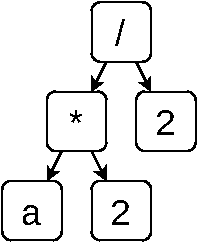
\includegraphics[height=3cm]{ast}}
  \subcaptionbox{Term graph with sharing.\label{fig:ast2}}
    [0.5\linewidth]{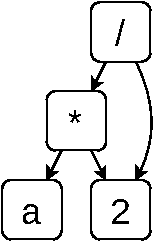
\includegraphics[height=3cm]{ast-sharing}}
  \caption{
    Different representations of the program $(a * 2) / 2$ have
     different characteristics.
    The syntax tree is simpler \subref{fig:ast1},
     but the term graph is smaller since it captures sharing \subref{fig:ast2}.
  }\label{fig:ast}
\end{figure}

\begin{quote}
  \it\Thesisstmt
\end{quote}

\hrule

Equality graphs (\egraphs) were originally developed to
  efficiently represent congruence relations
  in automated theorem provers (ATPs).
At a high level, \egraphs~\cite{nelson, pp-congr}
  extend union-find~\cite{unionfind} to compactly represent
  equivalence classes of expressions while
  maintaining a key invariant:
  the equivalence relation is closed under congruence.\footnote{
    Intuitively, congruence simply means
    that $a \equiv b$ implies $f(a) \equiv f(b)$.}

Over the past decade, several projects have repurposed \egraphs
  to implement state-of-the-art, rewrite-driven
  compiler optimizations and program synthesizers
  using a technique known as \textit{equality saturation}~\cite{
    denali, eqsat, eqsat-llvm, szalinski, yogo-pldi20, spores, herbie}.
Given an input program $p$,
  equality saturation constructs an \egraph $E$ that
  represents a large set of programs equivalent to $p$,
  and then extracts the ``best'' program from $E$.
The \egraph is grown by repeatedly applying
  pattern-based rewrites. % $\ell \to r$.
%Each rewrite $\ell \to r$ includes
%  a pattern $\ell$ to \textit{match} and
%  a pattern $r$ to instantiate and \textit{merge}
%  with the matched subterm.
Critically, these rewrites only add information to the \egraph,
  eliminating the need for careful ordering.
Upon reaching a fixed point (\textit{saturation}),
  $E$ will represent \textit{all equivalent ways} to
  express $p$ with respect to the given rewrites.
After saturation (or timeout),
  a final \textit{extraction} procedure
  analyzes $E$ and selects the
  optimal program according to
  a user-provided cost function.

Ideally, a user could simply provide
  a language grammar and rewrites,
  and equality saturation would produce a effective optimizer.
Two challenges block this ideal.
First, maintaining congruence can become expensive as $E$ grows.
In part, this is because \egraphs from the conventional ATP setting
  remain unspecialized to the distinct \textit{equality saturation workload}.
Second, many applications critically depend on
  \textit{domain-specific analyses}, but
  integrating them requires ad~hoc extensions to the \egraph.
The lack of a general extension mechanism
  has forced researchers to re-implement
  equality saturation from scratch several times~\cite{herbie, eqsat, wu_siga19}.
These challenges limit equality saturation's practicality.

\textit{Equality Saturation Workload. $\,$}
%
ATPs frequently query and modify \egraphs and
  additionally require \textit{backtracking} to
  undo modifications (e.g., in  DPLL(T)~\cite{dpll}).
These requirements force conventional \egraph designs
  to maintain the congruence invariant after every operation.
In contrast,
  the equality saturation workload does not require backtracking and
  can be factored into distinct phases of
  (1) querying the \egraph to simultaneously find all rewrite matches and
  (2) modifying the \egraph to merge in equivalences for all matched terms.

We present a new amortized algorithm
  called \textit{rebuilding} that defers \egraph invariant maintenance
  to equality saturation phase boundaries without compromising soundness.
Empirically, rebuilding provides asymptotic speedups
  over conventional approaches.

\textit{Domain-specific Analyses. $\,$}
%
Equality saturation is primarily driven by syntactic rewriting,
  but many applications require additional interpreted reasoning
  to bring domain knowledge into the \egraph.
Past implementations have resorted to
  ad~hoc \egraph manipulations
  to integrate what would otherwise be
  simple program analyses like constant folding.

To flexibly incorporate such reasoning,
  we introduce a new, general mechanism called \textit{\eclass analyses}.
An \eclass analysis annotates each \eclass
  (an equivalence class of terms)
  with facts drawn from a semilattice domain.
%  resembling an abstract interpretation lifted to \egraphs.
As the \egraph grows,
  facts are introduced, propagated, and joined
  to satisfy the \textit{\eclass analysis invariant},
  which relates analysis facts to the terms represented in the \egraph.
Rewrites cooperate with \eclass analyses by
  depending on analysis facts and
  adding equivalences that in turn
  establish additional facts.
Our case studies and examples
  (Sections \ref{sec:impl} and \ref{sec:case-studies})
  demonstrate \eclass analyses like
  constant folding and free variable analysis
  which required bespoke customization in
  previous equality saturation implementations.

\textit{\Egg. $\,$}
%
We implement rebuilding and \eclass analyses in
  an open-source\footnote{
    \begin{tabular}[t]{ll}
      web: & \url{https://egraphs-good.github.io}\\
      source: & \url{https://github.com/egraphs-good/egg}\\
      documentation: & \url{https://docs.rs/egg}
    \end{tabular}
  }
  library called \egg (\textbf{e}-\textbf{g}raphs \textbf{g}ood).
\Egg specifically targets equality saturation,
  taking advantage of its workload characteristics and
  supporting easy extension mechanisms to
  provide \egraphs specialized for
  program synthesis and optimization.
\Egg also addresses more prosaic challenges,
  e.g., parameterizing over user-defined
  languages, rewrites, and cost functions
  while still providing an optimized implementation.
Our case studies demonstrate how \egg's features
  constitute a general, reusable \egraph library that can
  support equality saturation across diverse domains.

\begin{samepage}
In summary, the contributions of this paper include:
\begin{itemize}
% \item Identifying that equality saturation
%   exposes \egraph to a workload different from
%   theorem provers~\cite{z3} and therefore can benefit from a
%   specialized algorithm for maintaining congruence.
\item Rebuilding (\autoref{sec:rebuilding}),
  a technique that restores key correctness and performance invariants
  only at select points in the equality saturation algorithm.
  Our evaluation demonstrates that rebuilding is faster than
  existing techniques in practice.

\item \Eclass analysis (\autoref{sec:extensions}),
  a technique for integrating domain-specific analyses
  that cannot be expressed as purely syntactic rewrites.
  The \eclass analysis invariant provides the guarantees
  that enable cooperation between rewrites and analyses.


%    a technique for maintaining additional information in \eclasses
%    that enables integrating domain-specific analyses
%    that cannot be expressed as syntactic rewrites.

% \item Identifying the key invariants necessary
%   for a correct, high-performance \egraph library for equality saturation.

\item A fast, extensible implementation of
  \egraphs in a library dubbed \egg (\autoref{sec:impl}).

\item Case studies of real-world, published tools that use \egg
    for deductive synthesis and program optimization across domains such as
    floating point accuracy,
    linear algebra optimization,
    and CAD program synthesis
    (\autoref{sec:case-studies}).
    Where previous implementations existed,
      \egg is orders of magnitude faster and offers more features.
\end{itemize}
\end{samepage}
% The rest of the paper is organized as follows:
% \autoref{sec:background} provides background on term rewriting
%   and defines \egraphs and the invariant, \congrinv.
% It describes the equality saturation workload and how it compares
%   to theorem proving.
% \autoref{sec:rebuild} introduces \egg's novel algorithm
%   for invariant maintenance called \textit{rebuilding}
%   and evaluates it to demonstrate the resulting speedups.
% \autoref{sec:extensions} introduces \eclass analysis and shows
%   how it is used for conditional and dynamic rewrites, and extraction.
% \autoref{sec:impl} discusses the implementation of \egg and
%   presents a partial evaluator for the lambda calculus implemented
%   using \egg.
% \autoref{sec:case-studies} presents three major research projects that
%   have used \egg as their equality saturation engine and benefited
%   in terms of performance and scalability.
% \autoref{sec:related} presents a summary of relevant related work and
% \autoref{sec:conclusion} concludes.


%\Zach{contributions}


%% At a high level, \egraphs~\cite{nelson, pp-congr} store expressions
%%   similarly to the union-find~\cite{unionfind} data structures
%%   often used for representing equivalence relations.
%% The key additional invariant maintained by the e-graph is that its
%%   equivalence relation is closed under congruence.

%  and a performance invariant ($\mathcal{I}_p$) ensuring that
%  equivalent terms are stored without duplication, i.e. equivalent
%  subterms are shared whenever possible.
% \Max{dedup isn't a necessary invariant, it's for perf}

%Equality saturation uses \egraphs to construct $E$,
%  but the resulting workload exhibits distinct phases compared to ATPs and
%  often requires ad~hoc extensions to integrate domain-specific analyses.

% Second, integrating domain-specific analyses
%   requires ad~hoc extensions to the \egraph.
% The lack of a general extension mechanism
%   complicates combining rewrites with analyses.
% These challenges limit equality saturation's practical applicability;
%   researchers have resorted to re-implementing
%   equality saturation from scratch for each new domain.



%%% Local Variables:
%%% TeX-master: "../thesis"
%%% End:

\chapter{Background}
\label{sec:background}

\section{Term Representation and Rewriting}

The most common and easily understood
 program representation is the venerable
 \textit{abstract syntax tree} (AST).
An AST is a recursive tree data structure
 where a node is an operator and
 some number---potentially zero---of children ASTs.
For example, the program $(a * 2) / 2$
 is represented by the AST shown in \autoref{fig:ast1}.
The operators $*$ and $/$ each take two children;
 the variable $a$ and the number $2$ are leaf operators
 that take no children.

ASTs are the primary data structures used in most programming tools,
 but they are not the only ones.
A common alternate representation is the \textit{term graph},
 which can be viewed as a variant of ASTs that loosens the tree requirement.
Term graphs can there for capture sharing across common parts of a
 program (also known as a term).
\autoref{fig:ast2} shows a term graph for the program $(a * 2) / 2$.
% Term graphs can be ``unfolded'' into ASTs be duplicating the shared subgraphs,
%  but the resulting ASTs can be exponentially larger than the term graph.

\begin{figure}
  \subcaptionbox{AST without sharing.\label{fig:ast1}}
    [0.5\linewidth]{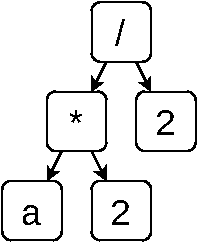
\includegraphics[height=3cm]{ast}}
  \subcaptionbox{Term graph with sharing.\label{fig:ast2}}
    [0.5\linewidth]{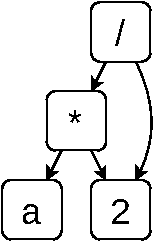
\includegraphics[height=3cm]{ast-sharing}}
  \caption{
    Different representations of the program $(a * 2) / 2$ have
     different characteristics.
    The syntax tree is simpler \subref{fig:ast1},
     but the term graph is smaller since it captures sharing \subref{fig:ast2}.
  }\label{fig:ast}
\end{figure}

Regardless of the choice of program representation,
 a common technique for program manipulation is rewriting.
In this paradigm,
 program transformations are given as a set of rewrites,
 where each
 rewrite $l \to r$ specifies a pattern $l$ to search for
 and a another pattern $r$ with
 which to replace each instance of $l$ found
 in the program.
For example, applying the rewrite $x * 2 \to x + x$
 to our term $(a * 2) / 2$ yields $(a + a) / 2$.

Rewriting offers an
 intuitive, compositional, and efficient
 method to transform programs
 that is used in programming tools of all shapes and sizes.
It is a well-researched technique with a wealth of literature,
 \max{add citations}
 but it is not without its pitfalls.
\autoref{sec:rewriting} discusses these in detail,
 but many of the difficulties boil down to the fact that
 term rewriting operates on \emph{one term at a time}.

\begin{figure}
  \centering
  \subcaptionbox{
    Another subfigure\label{fig:bad-rewrites-a}
  }{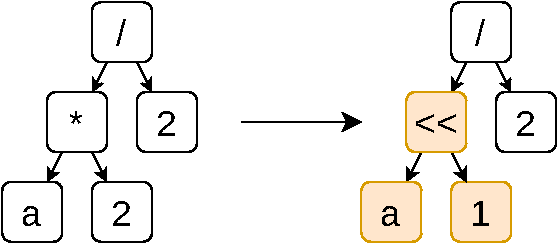
\includegraphics[height=35mm]{figures/bad-rewrites-a}}

  \vspace{1cm}
  \subcaptionbox{
    Another subfigure\label{fig:bad-rewrites-b}
  }{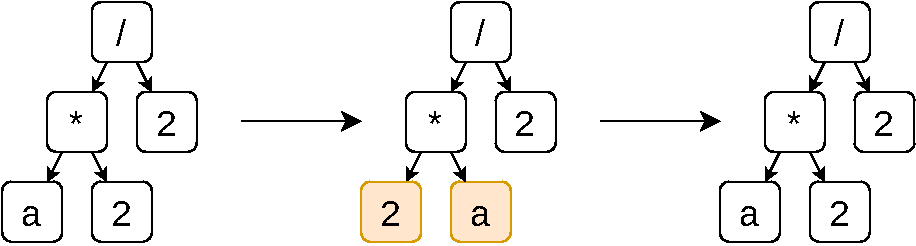
\includegraphics[height=35mm]{figures/bad-rewrites-b}}

  \vspace{1cm}
  \subcaptionbox{
    Another subfigure\label{fig:bad-rewrites-c}
  }{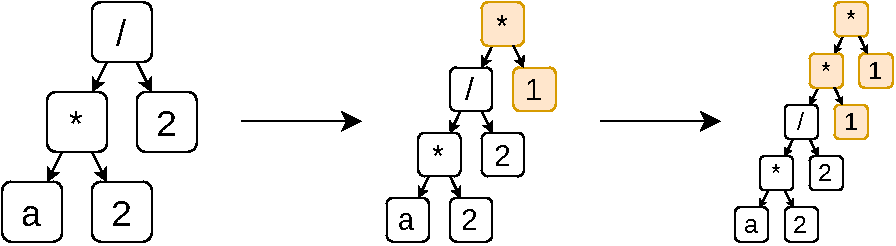
\includegraphics[height=35mm]{figures/bad-rewrites-c}}

  \caption{
    caption
  }\label{fig:bad-rewrites}
\end{figure}


\section{Term Rewriting}
\label{sec:rewriting}

\egg builds on \egraphs and equality saturation.
  This section describes those techniques and
  presents the challenges that \egg addresses.

% Many problems in program optimization, theorem proving,
%   and other domains have a similar shape:
% given an input expression, search for a ``better'' equivalent
%   expression.
% This paper puts forward the case that, with our proposed advances, equality
%   saturation is now the right tool for the job in many cases like
%   these.

% We will work through an extended example around optimizing
%   the expression
%   $(a \times 2) / 2$
%   and discover the benefits of \egraphs and equality saturation,
%   current limitations of using and implementing this approach,
%   and how \egg addresses those limitations.

\section{E-Graphs}
\label{sec:egraphs}

An \textit{\egraph} is a data structure that stores a set of terms and a
  congruence relation over those terms.
Originally developed for and still used in the
  heart of theorem provers~\cite{nelson, simplify, z3},
  \egraphs have also been used to power a program optimization technique
  called \textit{equality saturation}~%
  \cite{denali, eqsat, eqsat-llvm, szalinski, yogo-pldi20, spores, herbie}.

\subsection{Definitions}

\begin{figure}
  \centering
  \begin{align*}
     \text{function symbols} \quad & f,g                                   \\[-0.2em]
     \text{\eclass ids} \quad & a,b & \text{opaque identifiers}            \\[-0.2em]
     \text{terms}     \quad & t  ::= f \mid f(t_1, \ldots, t_m) & m \geq 1 \\[-0.2em]
     \text{\enodes}   \quad & n  ::= f \mid f(a_1, \ldots, a_m) & m \geq 1 \\[-0.2em]
     \text{\eclasses} \quad & c  ::= \{ n_1, \ldots, n_m \}     & m \geq 1
  \end{align*}
  \caption{
    Syntax and metavariables for the components of an \egraph.
    Function symbols may stand alone as constant \enodes and terms.
    An \eclass id is an opaque identifier that can be compared for equality with $=$.
  }
  \label{fig:syntax}
\end{figure}

Intuitively,
  an \egraph is a set of equivalence classes (\textit{\eclasses}).
Each \eclass is a set of \textit{\enodes} representing equivalent terms from a given language,
  and an \enode is a function symbol paired with a list of children \eclasses.
More precisely:

\begin{definition}[Definition of an E-Graph]
  \label{def:egraph}

  Given the definitions and syntax in \autoref{fig:syntax},
  an \textit{\egraph} is a tuple $(U, M, H)$ where:
  \begin{itemize}
    \item
    A union-find data structure~\cite{unionfind} $U$
      stores an equivalence relation (denoted with $\equivid$)
      over \eclass ids.

    \item
    The \textit{\eclass map} $M$ maps \eclass ids to \eclasses.
    All equivalent \eclass ids map to the same \eclass, i.e.,
      $a \equivid b$ iff $M[a]$ is the same set as $M[b]$.
    An \eclass id $a$ is said to \textit{refer to} the \eclass $M[\find(a)]$.

    \item The \textit{hashcons}\footnote{
      We use the term \textit{hashcons} to evoke the memoization technique,
      since both avoid creating new duplicates of existing objects.
    }
    $H$ is a map from \enodes to \eclass ids.
  \end{itemize}

  % An \textit{\eclass} is a set of \enodes.
  % An \textit{\enode} $f(a_{1}, ..., a_{n})$ is
  %   a function symbol $f$ from the given language
  %   and a (potentially empty) list of \eclass ids.

  Note that an e-class has an identity
   (its canonical \eclass id),
   but an \enode does not.\footnote{
    Our definition of an \egraph reflects \egg's design
      and therefore differs with some other \egraph definitions and implementations.
    In particular, making e-classes but not e-nodes identifiable is unique to
      our definition.
  }
  We use \eclass id $a$ and the \eclass $M[\find(a)]$ synonymously when clear from the context.

\end{definition}

\begin{definition}[Canonicalization]
    An \egraph's union-find $U$ provides a \find operation that canonicalizes \eclass ids
      such that ${\find(U, a) = \find(U, b)}$ iff ${a \equivid b}$.
    We omit the first argument of \find where clear from context.
    \begin{itemize}
      \item An \eclass id $a$ is canonical iff $\find(a) = a$.
      \item \raggedright
            An \enode $n$ is canonical iff $n = \texttt{canonicalize}(n)$,
            where ${\texttt{canonicalize}(f(a_{1}, a_{2}, ...)) = f(\find(a_{1}), \find(a_{2}), ...)}$.
    \end{itemize}
\end{definition}

\begin{definition}[Representation of Terms]
  An \egraph, \eclass, or \enode is said to \textit{represent} a term $t$ if $t$ can be
    ``found'' within it. Representation is defined recursively:
  \begin{itemize}
    \item An \egraph represents a term if any of its \eclasses do.
    \item An \eclass $c$ represents a term if any \enode $n \in c$ does.
    \item An \enode $f(a_{1}, a_{2}, ...)$ represents a term $f(t_{1}, t_{2}, ...)$
          if they have the same function symbol $f$
          and \eclass $M[a_{i}]$ represents term $t_{i}$.
  \end{itemize}

  When each \eclass is a singleton (containing only one \enode),
    an \egraph is essentially a term graph with sharing.
  \autoref{fig:egraph-rewrite1} shows an \egraph that represents the
    expression $(a \times 2) / 2$.
\end{definition}

\begin{definition}[Equivalence]
  An \egraph defines three equivalence relations.
  \begin{itemize}
    \item Over \eclass ids: $a \equivid b$ iff $\find(a) = \find(b)$.
    \item Over \enodes: $n_{1} \equivnode n_{2}$ iff \enodes $n_{1}, n_{2}$ are in the same \eclass,
          i.e., $\exists a.\ n_{1}, n_{2} \in M[a]$.
    \item Over terms: $t_{1} \equivterm t_{2}$ iff terms $t_{1}, t_{2}$ are represented in the same \eclass.
  \end{itemize}

  We use $\equiv$ without the subscript when the relation is clear from context.
\end{definition}

\begin{definition}[Congruence]
  For a given \egraph, let $\cong$ denote a congruence relation over \enodes such that
  ${f(a_{1}, a_{2}, ...) \cong f(b_{1}, b_{2}, ...)}$ iff $a_{i} \equivid b_{i}$.
  Let $\cong^{*}$ denote the congruence closure of $\equivnode$,
   i.e., the smallest superset of $\equivnode$ that is also a superset of $\cong$.
  Note that there may be two \enodes such that
    $n_{1} \cong^{*} n_{2}$ but
    $n_{1} \not\cong n_{2}$ and
    $n_{1} \not\equivnode n_{2}$.
  The relation $\cong$ only represents a single step of congruence;
  more than one step may be required to compute the congruence closure.
\end{definition}

\subsection{E-Graph Invariants}
\label{sec:invariants}

The \egraph must maintain invariants in order to
  correctly and efficiently implement the operations given in \autoref{sec:interface}.
This section only defines the invariants,
  discussion of how they are maintained is deferred to \autoref{sec:rebuild}.
These are collectively referred to as the \textit{e-graph invariants}.

\begin{definition}[The Congruence Invariant]
  \label{def:cong-inv}
  The equivalence relation over \enodes must be closed over congruence,
    i.e., $(\equivnode) = (\cong^{*})$.
  The \egraph must ensure that congruent \enodes are in the same \eclass.
  Since identical \enodes are trivially congruent,
   this implies that an \enode must be uniquely contained in a single \eclass.
\end{definition}

\begin{definition}[The Hashcons Invariant]
  \label{def:hash-inv}
  The hashcons $H$ must map all canonical \enodes to their \eclass ids.
  In other words:
  $$ \enode\ n \in M[a] \iff H[\texttt{canonicalize}(n)] = \find(a) $$
 % for each pair $(n, a) \in H$, \enode $n$ must be canonical and $n \in M[a]$.

  If the hashcons invariant holds, then a procedure $\texttt{lookup}$
    can quickly find which \eclass (if any) has an \enode congruent to a given \enode $n$:
  $\texttt{lookup}(n) = H[\texttt{canonicalize}(n)]$.
\end{definition}

%   \Remy{How can add violate deduplication?}
% Traditionally, \egraphs employ two techniques to maintain the invariants on
%   every call to \texttt{add} or \texttt{merge}.

% As \eclasses grow, the \egraph represents exponentially (or even infinitely) many terms,
%   one for every choice of representative \enode for each \eclass.
% The \egraph in \autoref{fig:egraph-rewrite-before} is essentially an AST with
%   sharing, since each \eclass is a singleton.

% \Egraphs are manipulated by two main operations:
%   adding new \enodes (into new \eclasses)
%   and merging \eclasses (sometimes called \textit{asserting} equivalences).
% \Chandra{since this is POPL, I feel that we might be expected to
% write invariants like the following a bit more formally?}
% These operations maintain two important invariants, which we will call the
%   \textit{\egraph invariants}:
% \begin{enumerate}
%   \item Deduplication:
%     The \egraph must not contain two \enodes with the same operator and
%     equivalent children.
%     \Leo{clarify dedup; distinguish identical and equivalent}
%     \Leo{this doesn't necessarity hold in modern \egraphs}
%   \item Congruence:
%     The equivalence relation on terms must also be a congruence relation, i.e.
%     if $a = b$ then $f(a) = f(b)$.
% \end{enumerate}

% Both operations can violate the two \egraph's congruence invariant.

% Deduplication is typically maintained by \textit{hashconsing}, or memoizing,
%   the add operation.
% If the user tries to add an \enode that is already represented in the \egraph,
%   the \egraph should simply return the \eclass representing the \enode instead of
%   inserting the \enode.
% Congruence is traditionally maintained by keeping a list of
%   \textit{parent pointers} for each \eclass that stores which \enodes have that
%   \eclass as children.
% On the merge operation, the parents of the merged classes must be checked to see
%   if any pairs of them became equivalent, proceeding recursively until no
%   additional equivalences are found.

\begin{figure}
  \begin{subfigure}[t]{0.45\linewidth}
    \centering
    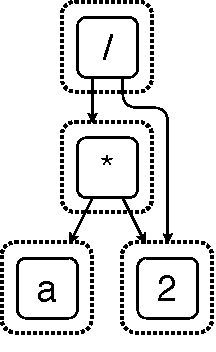
\includegraphics[height=50mm]{overview1.pdf}
    \caption{Initial \egraph contains ${(a \times 2) / 2}$.}
    \label{fig:egraph-rewrite1}
  \end{subfigure}
  \hfill
  \begin{subfigure}[t]{0.45\linewidth}
    \centering
    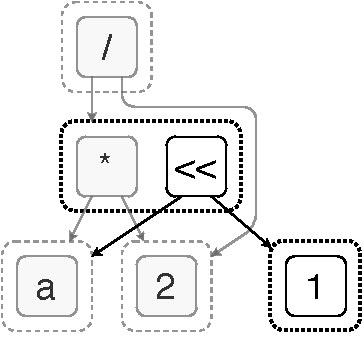
\includegraphics[height=50mm]{overview2.pdf}
    \caption{
      Applied ${x \times 2 \to x \ll 1}$.
    }\label{fig:egraph-rewrite2}
  \end{subfigure}
  \\[1em]
  \begin{subfigure}[t]{0.45\linewidth}
    \centering
    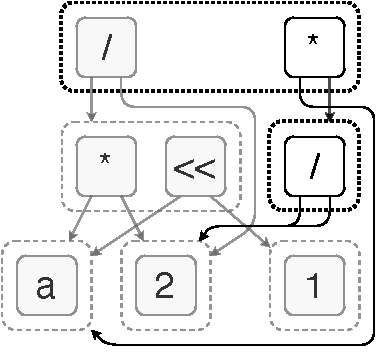
\includegraphics[height=50mm]{overview3.pdf}
    \caption{
      Applied rewrite ${(x \times y) / z \to x \times (y / z)}$.
    }\label{fig:egraph-rewrite3}
  \end{subfigure}
  \hfill
  \begin{subfigure}[t]{0.45\linewidth}
    \centering
    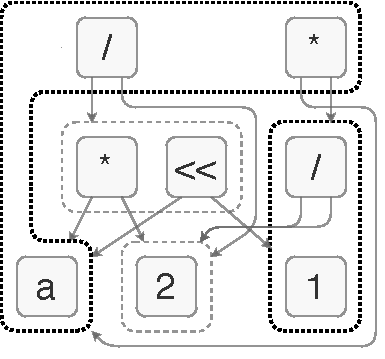
\includegraphics[height=50mm]{overview4.pdf}
    \caption{
      Applied ${x / x \to 1}$ and ${1 \times x \to x}$.
    }\label{fig:egraph-rewrite4}
  \end{subfigure}
  \caption{
    An \egraph consists of \eclasses (dashed boxes) containing
      equivalent \enodes (solid boxes).
    Edges connect \enodes to their child \eclasses.
    Additions and modifications are emphasized in black.
    Applying rewrites to an \egraph adds new \enodes and edges,
      but nothing is removed.
    Expressions added by rewrites are merged with the matched \eclass.
    In \autoref{fig:egraph-rewrite4}, the rewrites do not add any new nodes,
      only merge \eclasses.
    The resulting \egraph has a cycle,
      representing infinitely many expressions:
      $a$, $a \times 1$, $a \times 1 \times 1$, and so on.
  }
  \label{fig:egraph-rewrite}
\end{figure}

\subsection{Interface and Rewriting}
\label{sec:interface}

\Egraphs bear many similarities to the classic union-find data
  structure that they employ internally,
  and they inherit much of the terminology.
\Egraphs provide two main low-level mutating operations:
\begin{itemize}
    \item \texttt{add} takes an \enode $n$ and:
    \begin{itemize}
        \item if $\texttt{lookup}(n) = a$, return $a$;
        \item if $\texttt{lookup}(n) = \emptyset$,
              then set $M[a] = \{ n \}$ and return the id $a$.
    \end{itemize}
    \item \texttt{merge} (sometimes called \texttt{assert} or \texttt{union})
    takes two \eclass ids $a$ and $b$,
    unions them in the union-find $U$,
    and combines the \eclasses by setting both $M[a]$ and $M[b]$ to $M[a] \cup M[b]$.
\end{itemize}

Both of these operations must take additional steps to maintain the congruence
  invariant.
Invariant maintenance is discussed in \autoref{sec:rebuilding}.

\Egraphs also offers operations for querying the data structure.
\begin{itemize}
    \item \texttt{find} canonicalizes \eclass ids using the union-find $U$ as described in definition \ref{def:egraph}.
    \item \texttt{ematch} performs the
          \textit{e-matching}~\cite{simplify, ematching}
          procedure for finding patterns in the \egraph.
          \texttt{ematch} takes a pattern term $p$ with variable placeholders
          and returns a list of tuples $(\sigma, c)$ where $\sigma$ is a substitution of
          variables to \eclass ids such that $p[\sigma]$ is represented in \eclass $c$.
\end{itemize}
These can be composed to perform rewriting over the
  \egraph.
To apply a rewrite $\ell \to r$ to an \egraph,
  \texttt{ematch}
  finds tuples $(\sigma, c)$ where \eclass $c$ represents $\ell[\sigma]$.
Then, for each tuple,
  \mbox{\texttt{merge($c$, add($r[\sigma]$))}} adds $r[\sigma]$ to the \egraph
  and unifies it with the matching \eclass c.

\autoref{fig:egraph-rewrite} shows an \egraph undergoing a series of rewrites.
Note how the process is only additive; the initial term $(a \times 2) / 2$ is
  still represented in the \egraph.
Rewriting in an \egraph can also saturate, meaning the \egraph has
  learned every possible equivalence derivable from the given rewrites.
% This not only solves the phase ordering problem, but also handles rules like
%   commutativity that can be troublesome to a conventional rewrite system.
If the user tried to apply $x \times y \to y \times x$ to an \egraph twice,
  the second time would add no additional \enodes and perform no new merges;
  the \egraph can detect this and stop applying that rule.

\section{Equality Saturation}
\label{sec:eqsat}

Term rewriting~\cite{nachum-rewrites} is a time-tested approach
  for equational reasoning in
  program optimization~\cite{eqsat, denali},
  theorem proving~\cite{simplify, z3},
  and program transformation~\cite{graphs}.
In this setting, a tool repeatedly chooses one of a set of axiomatic rewrites,
  searches for matches of the left-hand pattern in the given
  expression, and replaces matching instances with the substituted
  right-hand side.

Term rewriting is typically destructive and ``forgets'' the matched
  left-hand side.
Consider applying a simple strength reduction rewrite:
  ${ (a \times 2) / 2 \to (a \ll 1) / 2 }$.
The new term carries no
  information about the initial term.
Applying strength reduction at this point prevents us from canceling out $2/2$.
In the compilers community, this classically tricky question of when to apply
  which rewrite is called the \textit{phase ordering} problem.

One solution to the phase ordering problem would simply apply all
  rewrites simultaneously, keeping track of every expression seen.
This eliminates the problem of choosing the right rule, but
  a naive implementation would require space exponential in the number
  of given rewrites.
\textit{Equality saturation}~\cite{eqsat, eqsat-llvm} is a technique to do this
  rewriting efficiently using an \egraph.

\begin{figure}
  \centering
  \begin{lstlisting}[language=Python, gobble=4, numbers=left, basicstyle=\small\ttfamily, xleftmargin=40mm]
    def equality_saturation(expr, rewrites):
      egraph = initial_egraph(expr)

      while not egraph.is_saturated_or_timeout():

        for rw in rewrites:
          for (subst, eclass) in egraph.ematch(rw.lhs):
            eclass2 = egraph.add(rw.rhs.subst(subst))
            egraph.merge(eclass, eclass2)

      return egraph.extract_best()
  \end{lstlisting}
  \caption{
    Pseudocode for equality saturation.
    Traditionally, equality saturation maintains the \egraph data structure
      invariants throughout the algorithm.
  }
  \label{fig:eq-sat-bg}
\end{figure}

\autoref{fig:eq-sat-bg} shows the equality saturation workflow.
First, an initial \egraph is created from the input term.
The core of the algorithm runs a set of rewrite rules until the \egraph is
  saturated (or a timeout is reached).
Finally, a procedure called \textit{extraction} selects the optimal represented
  term according to some cost function.
For simple cost functions, a bottom-up, greedy traversal of the \egraph suffices
  to find the best term.
Other extraction procedures have been explored for more complex cost
  functions~\cite{spores, wu_siga19}.

Equality saturation eliminates the tedious and often error-prone
  task of choosing when to apply which rewrites,
%Equality saturation turns a correctness problem into a performance problem,
  promising an appealingly simple workflow: state the
  relevant rewrites for the language, create an initial \egraph from a given
  expression, fire the rules until saturation,
  and finally extract the cheapest equivalent expression.
Unfortunately, the technique remains ad hoc; prospective equality saturation
  users must implement their own \egraphs customized to their language, avoid
  performance pitfalls, and hack in the ability to do interpreted reasoning
  that is not supported by purely syntactic rewrites.
\egg aims to address each aspect of these difficulties.

\section{Equality Saturation and Theorem Proving}

An equality saturation engine and a theorem prover each have capabilities that
  would be impractical to replicate in the other.
Automated theorem provers like satisfiability modulo theory (SMT) solvers are
  general tools that, in addition to supporting satisfiability queries,
  incorporate sophisticated, domain-specific solvers to allow interpreted
  reasoning within the supported theories.
On the other hand, equality saturation is specialized for optimization, and its
  extraction procedure directly produces an optimal term with respect to a given
  cost function.
% To replicate extraction with an SMT solver, one would have to resort to a more
%   expensive enumerative approach.

% \James{What enumerative approach? How do you know that one would "have to" resort to it?}

While SMT solvers are indeed the more general tool,
  equality saturation is not superseded by SMT;
  the specialized approach can be much faster when the full generality of SMT is
  not needed.
To demonstrate this, we replicated a portion of the recent TASO paper~\cite{taso},
  which optimizes deep learning models.
As part of the work, they must verify a set of synthesized equalities with
  respect to a trusted set of universally quantified axioms.
TASO uses Z3~\cite{z3} to perform the
  verification even though most of Z3's features
  (disjunctions, backtracking, theories, etc.)
  were not required.
An equality saturation engine can also be used for verifying these equalities
  by adding the left and right sides of
  each equality to an \egraph,
  running the axioms as rewrites,
  and then checking if both sides end up in the same \eclass.
Z3 takes 24.65 seconds to perform the verification;
  \egg performs the same task in 1.56 seconds ($15\times$ faster),
  or only 0.52 seconds ($47\times$ faster) when using
  \egg's batched evaluation (\autoref{sec:egg-batched}).

% \James{
  % The experimental/perf numbers in the last par of 2.4 feel out of place. Not sure how to fix...
% }

% However, their abilities overlap on a specific kind of theorem proving:
%   given a list of axioms in the form of universal quantified equalities,
%   prove two (or more) terms equal.
% Some SMT solvers support these kinds of queries, albeit in a limited fashion
%   since they are undecidable.
% \footnotetext{
%   Since these queries are undecidable, both SMT solvers and equality
%   saturation engines can either prove the inputs equal or fail to; they cannot
%   prove them unequal.
% }



%%% Local Variables:
%%% TeX-master: "../thesis"
%%% End:

\chapter{Rebuilding: A New Take on \Egraph Invariant Maintenance}
\label{sec:rebuild}
\label{sec:rebuilding}

% Rebuilding is a new, general perspective on \egraph invariant maintenance.
Traditionally~\cite{nelson, simplify},
  \egraphs maintain their data structure invariants
  after each operation.
We separate this invariant restoration into a procedure called \textit{rebuilding}.
This separation allows the client to
  choose when to enforce the \egraph invariants.
Performing a rebuild immediately after every operation replicates the
  traditional approach to invariant maintenance.
In contrast, rebuilding less frequently can amortize the cost of invariant
  maintenance, significantly improving performance.

In this section, we first describe how e-graphs have
  traditionally maintained invariants (\autoref{sec:upward}).
We then describe the rebuilding framework and how it captures a spectrum of
  invariant maintenance approaches, including the traditional one
  (\autoref{sec:rebuilding-detail}).
Using this flexibility, we then give a modified algorithm for equality
  saturation that enforces the \egraph invariants at only select points
  (\autoref{sec:rebuilding-eqsat}).
We finally demonstrate that this new approach offers an asymptotic speedup over
  traditional equality saturation (\autoref{sec:rebuild-eval}).

% Among \egg's optimizations (\autoref{sec:egg-efficient}),
%   strategically delayed rebuilding is perhaps the most important.
% \egg employed a m
% Delayed rebuilding amortizes the cost of invariant maintenance, significantly reducing work

% Rebuilding is a novel technique that lies at the heart of \egg's
%   modified equality saturation algorithm.
% This crucial technique allows equality saturation to specialize the \egraph to
%   its workload, yielding substantial performance improvements.
%   %from both an algorithmic and implementation
%   %perspective.

% Rebuilding gives the user (or algorithm) choice on when to restore the \egraph
%   invariants, which can have a large impact on performance .

% The key insight is that maintaining the \egraph invariants is expensive, and

% \autoref{fig:eq-sat-code} shows both the traditional and \egg's modified
%   equality saturation loop.
% The key distinction is \textit{when} the \egraph invariants of deduplication and
%   congruence are maintained.
% In traditional \egraphs, like with many data structures, invariants always
%   hold.
% In contrast, mutating an \egg \egraph may violate invariants, causing equalities
%   to be not ``seen'' when searching for patterns.
% \egg lets the user (or the algorithm) choose when to restore the invariants by
%   calling the \texttt{rebuild} method.
% Rebuilding leads to a lower amortized cost of maintaining the \egraph invariants.

\section{Upward Merging}
\label{sec:upward}

Both mutating operations on the \egraph
  (\texttt{add} and \texttt{merge}, \autoref{sec:interface})
  can break the \egraph invariants if not done carefully.
\Egraphs have traditionally used \textit{hashconsing} and
  \textit{upward merging} to maintain the congruence invariant.

The \texttt{add} operation relies on the hashcons invariant
  (Definition \ref{def:hash-inv})
  to quickly check whether the \enode $n$ to be added---or one congruent to it---is
  already present.
Without this check, \texttt{add} would create a new \eclass with $n$ in it
  even if some $n' \cong n$ was already in the \egraph,
  violating the congruence invariant.

The \texttt{merge} operation \eclasses can violate both \egraph invariants.
If $f(a, b)$ and $f(a, c)$ reside in two different \eclasses $x$ and $y$,
  merging $b$ and $c$ should also merge $x$ and $y$ to maintain the congruence invariant.
This can propagate further, requiring additional merges.

 % merging $x$ and $y$ could cause two other
 %  \enodes to become congruent and require merging their \eclasses.

\Egraphs maintain a \textit{parent list} for each \eclass
  to maintain congruence.
The parent list for \eclass $c$ holds all \enodes that have $c$ as a child.
When merging two \eclasses, \egraphs inspect these parent lists to find parents
  that are now congruent, recursively ``upward merging'' them if necessary.

The \texttt{merge} routine must also perform bookkeeping to preserve the
  hashcons invariant.
In particular, merging two \eclasses may change how parent \enodes of those
  \eclasses are canonicalized.
The \texttt{merge} operation must therefore
  remove, re-canonicalize, and replace those \enodes in the
  hashcons.
In existing \egraph implementations~\cite{herbie} used for equality saturation,
  maintaining the invariants while merging can take the vast majority of
  run time.

\section{Rebuilding in Detail}
\label{sec:rebuilding-detail}

\begin{figure}
  \begin{minipage}[t]{0.47\linewidth}
    \begin{lstlisting}[gobble=4, numbers=left, basicstyle=\scriptsize\ttfamily, escapechar=|, xleftmargin=13pt, numbersep=7pt]
    def add(enode):
      enode = self.canonicalize(enode)
      if enode in self.hashcons:
        return self.hashcons[enode]
      else:
        eclass_id = self.new_singleton_eclass(enode)
        for child in enode.children:
          child.parents.add(enode, eclass_id)
        self.hashcons[enode] = eclass_id
        return eclass_id

    def merge(id1, id2)
      if self.find(id1) == self.find(id2):
        return self.find(id1)
      new_id = self.union_find.union(id1, id2)
      # traditional egraph merge can be
      # emulated by calling rebuild right after
      # adding the eclass to the worklist
      self.worklist.add(new_id) |\label{line:worklist-add}|
      return new_id

    def canonicalize(enode) |\label{line:canon}|
      new_ch = [self.find(e) for e in enode.children]
      return mk_enode(enode.op, new_ch)

    def find(eclass_id):
      return self.union_find.find(eclass_id)
    \end{lstlisting}
  \end{minipage}
  \hfill
  \begin{minipage}[t]{0.45\linewidth}
    \begin{lstlisting}[gobble=4, numbers=left, firstnumber=27, basicstyle=\scriptsize\ttfamily, numbersep=7pt]
    def rebuild():
      while self.worklist.len() > 0:
        # empty the worklist into a local variable
        todo = take(self.worklist)
        # canonicalize and deduplicate the eclass refs
        # to save calls to repair
        todo = { self.find(eclass) for eclass in todo }
        for eclass in todo:
          self.repair(eclass)

    def repair(eclass):
      # update the hashcons so it always points
      # canonical enodes to canonical eclasses
      for (p_node, p_eclass) in eclass.parents:
        self.hashcons.remove(p_node)
        p_node = self.canonicalize(p_node)
        self.hashcons[p_node] = self.find(p_eclass)

      # deduplicate the parents, noting that equal
      # parents get merged and put on the worklist
      new_parents = {}
      for (p_node, p_eclass) in eclass.parents:
        p_node = self.canonicalize(p_node)
        if p_node in new_parents:
          self.merge(p_eclass, new_parents[p_node])
        new_parents[p_node] = self.find(p_eclass)
      eclass.parents = new_parents
    \end{lstlisting}
  \end{minipage}
  \caption{
    Pseudocode for the \texttt{add}, \texttt{merge}, \texttt{rebuild}, and
    supporting methods.
    In each method, \texttt{self} refers to the \egraph being modified.
  }
  \label{fig:rebuild-code}
\end{figure}

Traditionally, invariant restoration is part of the
  \texttt{merge} operation itself.
Rebuilding separates these concerns,
  reducing \texttt{merge}'s obligations
  and allowing for amortized invariant maintenance.
In the rebuilding paradigm,
  \texttt{merge} maintains a \textit{worklist} of \eclass ids that need to
  be ``upward merged'', i.e., \eclasses whose parents are possibly congruent but
  not yet in the same \eclass.
The \texttt{rebuild} operation processes this worklist, restoring the invariants
  of deduplication and congruence.
Rebuilding is similar to other approaches in how it restores congruence
  (see \nameref{sec:related} for comparison to \cite{downey-cse});
  but it uniquely allows the client to choose when to restore invariants in the
  context of a larger algorithm like equality saturation.

\autoref{fig:rebuild-code} shows pseudocode for the main \egraph operations and
  rebuilding.
Note that \texttt{add} and \texttt{canonicalize} are given for completeness, but
  they are unchanged from the traditional \egraph implementation.
The \texttt{merge} operation is similar, but it only adds the new \eclass to the
  worklist instead of immediately starting upward merging.
Adding a call to \texttt{rebuild} right after the addition to
  the worklist (\autoref{fig:rebuild-code} line \ref{line:worklist-add})
  would yield the traditional behavior of restoring the invariants immediately.

The \texttt{rebuild} method essentially calls \texttt{repair} on the \eclasses
  from the worklist until the worklist is empty.
Instead of directly manipulating the worklist, \egg's \texttt{rebuild} method
  first moves it into a local variable and deduplicates \eclasses
  up to equivalence.
Processing the worklist may \texttt{merge} \eclasses,
  so breaking the worklist into chunks ensures that \eclass ids made
  equivalent in the previous chunk are deduplicated in the subsequent chunk.

The actual work of \texttt{rebuild} occurs in the \texttt{repair} method.
\texttt{repair} examines an \eclass $c$ and first canonicalizes \enodes in the
  hashcons that have $c$ as a child.
Then it performs what is essentially one ``layer'' of upward
  merging:
if any of the parent \enodes have become congruent, then their
  \eclasses are merged and the result is added to the worklist.

Deduplicating the worklist, and thus reducing calls to \texttt{repair},
  is at the heart of why deferring rebuilding improves
  performance.
Intuitively, the upward merging process of rebuilding traces out a ``path'' of
  congruence through the \egraph.
When rebuilding happens immediately after \texttt{merge}
  (and therefore frequently), these paths can substantially overlap.
By deferring rebuilding, the chunk-and-deduplicate approach can coalesce the
overlapping parts of these paths, saving what would have been redundant work.
In our modified equality saturation algorithm (\autoref{sec:rebuilding-eqsat}),
  deferred rebuilding is responsible for a significant, asymptotic speedup
  (\autoref{sec:rebuild-eval}).

\subsection{Examples of Rebuilding}

Deferred rebuilding speeds up congruence maintenance by amortizing the work of
  maintaining the hashcons invariant.
Consider the following terms in an \egraph:
  $f_{1}(x), ..., f_{n}(x),\, y_{1}, ..., y_{n}$.
Let the workload be $\texttt{merge}(x, y_{1}), ..., \texttt{merge}(x, y_{n})$.
Each merge may change the canonical representation of the $f_{i}(x)$s,
  so the traditional invariant maintenance strategy
  could require $O(n^{2})$ hashcons updates.
With deferred rebuilding the \texttt{merges} happen before
  the hashcons invariant is restored,
  requiring no more than $O(n)$ hashcons updates.

Deferred rebuilding can also reduce the number of calls to \texttt{repair}.
Consider the following $w$ terms in an \egraph,
  each nested under $d$ function symbols:
  $$f_1 (f_2(\ldots f_d(x_1))), \quad\ldots,\quad f_1(f_2(\ldots f_d(x_w)))$$
Note that $w$ corresponds the width of this group of terms, and $d$ to the depth.
Let the workload be $w-1$ merges that merge all the $x$s together:
  for $i \in [2, w], \texttt{merge}(x_{1}, x_{i})$.

In the traditional upward merging paradigm
  where \texttt{rebuild} is called after every \texttt{merge},
  each $\texttt{merge}(x_i, x_j)$ will require $O(d)$ calls to \texttt{repair}
  to maintain congruence, one for each layer of $f_{i}$s.
Over the whole workload, this requires $O(wd)$ calls to \texttt{repair}.

With deferred rebuilding, however, the $w-1$ merges can all take place before
  congruence must be restored.
Suppose the $x$s are all merged into an \eclass $c_{x}$
When \texttt{rebuild} finally is called,
  the only element in the deduplicated worklist is $c_{x}$.
Calling \texttt{repair} on $c_{x}$ will merge the \eclasses of the $f_{d}$
  \enodes into an \eclass $c_{f_{d}}$,
  adding the \eclasses that contained those \enodes back to the worklist.
When the worklist is again deduplicated,
  $c_{f_{d}}$ will be the only element,
  and the process repeats.
Thus, the whole workload only incurs $O(d)$ calls to \texttt{repair},
  eliminating the factor corresponding to the width of this group of terms.
\autoref{fig:repair-plot} shows that the number calls to \texttt{repair} is
  correlated with time spent doing congruence maintenance.

\subsection{Proof of Congruence}

Intuitively, rebuilding is a delay of the upward merging process, allowing
  the user to choose when to restore the \egraph invariants.
They are substantially similar in structure, with a critical a difference in when
  the code is run.
Below we offer a proof demonstrating that rebuilding restores the
\egraph congruence invariant.

\begin{theorem}
  Rebuilding restores congruence and terminates.
\end{theorem}

\begin{proof}
  Since rebuilding only merges congruent nodes,
    the congruence closure $\cong^{*}$ is fixed even though $\equivnode$ changes.
  When $(\equivnode) = (\cong^*)$, congruence is restored.
  Note that both $\equivnode$ and $\cong^*$ are finite.
  We therefore show that rebuilding causes $\equivnode$ to approach $\cong^*$.
  We define the set of incongruent \enode pairs as $I = (\cong^*) \setminus (\equivnode)$;
  in other words,
    $(n_{1}, n_{2}) \in I$ if $n_{1} \cong^{*} n_{2}$
     but $n_{1} \not\equivnode n_{2}$.
%    have the same function symbol
%    and equivalent children, but are not yet in the same \eclass.

  Due to the additive nature of equality saturation, $\equivnode$ only increases
    and therefore $I$ is non-increasing.
  However, a call to \texttt{repair} inside the loop of \texttt{rebuild} does
    not necessarily shrink $I$.
  Some calls instead remove an element from the worklist but do not modify the
    \egraph at all.

  Let the set $W$ be the worklist of \eclasses to be processed by
    \texttt{repair};
  in \autoref{fig:rebuild-code}, $W$ corresponds to \texttt{self.worklist} plus
    the unprocessed portion of the \texttt{todo} local variable.
  We show that each call to \texttt{repair} decreases the tuple
    $(|I|, |W|)$ lexicographically until $(|I|, |W|) = (0, 0)$,
    and thus rebuilding terminates with $(\equivnode) = (\cong^*)$.

  % If $I$ is empty, then $E = C$ by the definition of $I$, and the \egraph is
  %   congruent.
  % We show that, after rebuilding, both $I$ and $W$ are empty.

  Given an \eclass $c$ from $W$, \texttt{repair} examines $c$'s parents
    for congruent \enodes that are not yet in the same \eclass:
  \begin{itemize}
    \item If at least one pair of $c$'s parents are congruent,
          rebuilding merges each pair $(p_{1}$, $p_{2})$,
          which adds to $W$ but makes $I$ smaller by definition.
    \item If no such congruent pairs are found, do nothing.
          Then, $|W|$ is decreased by 1 since $c$ came from the
          worklist and \texttt{repair} did not add anything back.
  \end{itemize}

  Since $(|I|, |W|)$ decreases lexicographically,
    $|W|$ eventually reaches $0$, so \texttt{rebuild} terminates.
  Note that $W$ contains precisely those \eclasses that need to be
    ``upward merged'' to check for congruent parents.
  So, when $W$ is empty,
    \texttt{rebuild} has effectively performed upward merging.
%    albeit at a different time.
  By~\cite[Chapter 7]{nelson}, $|I| = 0$.
%    and is correct as per Nelson's
%  We therefore defer to Nelson's correctness
%    proof of the traditional upward merging algorithm
%    (Chapter 7, \cite{nelson})
%    to show that $|W| = 0$ implies $|I| = 0$.
Therefore, when rebuilding terminates, congruence is restored.

%  The \texttt{rebuild} method calls \texttt{repair} until $W$ is empty, so it
%  terminates.
%  If an \eclass had potentially incongruent parents,
%    then the \eclass would be in $W$.
%  Thus, if $W$ is empty, then no \eclasses have parents with incongruent \enodes,
%    so $I$ is empty as well,
%    and congruence is restored.
\end{proof}

\section{Rebuilding and Equality Saturation}
\label{sec:rebuilding-eqsat}

Rebuilding offers the choice of when to enforce the \egraph invariants,
  potentially saving work if deferred thanks to the deduplication of the
  worklist.
The client is responsible for rebuilding at a time that
  maximizes performance without limiting the application.

\begin{figure}
  \begin{subfigure}[t]{0.47\linewidth}
    \begin{lstlisting}[language=Python, gobble=6, numbers=left, basicstyle=\scriptsize\ttfamily, xleftmargin=13pt, numbersep=7pt]
      def equality_saturation(expr, rewrites):
        egraph = initial_egraph(expr)

        while not egraph.is_saturated_or_timeout():


          # reading and writing is mixed
          for rw in rewrites:
            for (subst, eclass) in egraph.ematch(rw.lhs):

              # in traditional equality saturation,
              # matches can be applied right away
              # because invariants are always maintained
              eclass2 = egraph.add(rw.rhs.subst(subst))
              egraph.merge(eclass, eclass2)

              # restore the invariants after each merge
              egraph.rebuild()

        return egraph.extract_best()
    \end{lstlisting}
    \caption{
      Traditional equality saturation alternates between searching and applying
      rules, and the \egraph maintains its invariants throughout.
    }
    \label{fig:eq-sat-code1}
  \end{subfigure}
  \hfill
  \begin{subfigure}[t]{0.47\linewidth}
    \begin{lstlisting}[language=Python, gobble=6, basicstyle=\scriptsize\ttfamily, numbers=left, numbersep=5pt]
      def equality_saturation(expr, rewrites):
        egraph = initial_egraph(expr)

        while not egraph.is_saturated_or_timeout():
          matches = []

          # read-only phase, invariants are preserved
          for rw in rewrites:
            for (subst, eclass) in egraph.ematch(rw.lhs):
              matches.append((rw, subst, eclass))

          # write-only phase, temporarily break invariants
          for (rw, subst, eclass) in matches:
            eclass2 = egraph.add(rw.rhs.subst(subst))
            egraph.merge(eclass, eclass2)

          # restore the invariants once per iteration
          egraph.rebuild()

        return egraph.extract_best()
    \end{lstlisting}
    \caption{
      \egg splits equality saturation iterations into read and write phases.
      The \egraph invariants are not constantly maintained, but restored
      only at the end of each iteration by the \texttt{rebuild} method
      (\autoref{sec:rebuild}).
    }
    \label{fig:eq-sat-code2}
  \end{subfigure}

  \caption{
    Pseudocode for traditional and \egg's version of the equality saturation
    algorithm.
  }
  \label{fig:eq-sat-code}
\end{figure}

\egg provides a modified equality saturation algorithm to take advantage
  of rebuilding.
\autoref{fig:eq-sat-code} shows pseudocode for both traditional equality
  saturation and \egg's variant, which exhibits two key differences:
\begin{enumerate}
  \item Each iteration is split into a read phase, which searches for all the
        rewrite matches, and a write phase that applies those matches.\footnote
    {
      Although the original equality saturation paper~\cite{eqsat}
      does not have separate reading and writing phases,
      some \egraph implementations (like the one inside Z3~\cite{z3})
      do separate these phases as an implementation detail.
      Ours is the first algorithm to take advantage of this by deferring
      invariant maintenance.
    }
  \item Rebuilding occurs only once per iteration, at the end.
\end{enumerate}

\egg's separation of the read and write phases means that rewrites are truly
  unordered.
In traditional equality saturation, later rewrites in the given rewrite list are
  favored in the sense that they can ``see'' the results of earlier rewrites in
  the same iteration.
Therefore, the results depend on the order of the rewrite list
  if saturation is not reached (which is common on large rewrite lists or input
  expressions).
\egg's equality saturation algorithm is invariant to the order of the rewrite
  list.

Separating the read and write phases also allows \egg to safely defer rebuilding.
If rebuilding were deferred in the traditional equality saturation algorithm,
  rules later in the rewrite list would be searched against an \egraph with
  broken invariants.
Since congruence may not hold, there may be missing equivalences, resulting in
  missing matches.
These matches will be seen after the \texttt{rebuild} during the next iteration
  (if another iteration occurs), but the false reporting could impact metrics
  collection, rule scheduling,\footnotemark{} or saturation detection.
\footnotetext{
  An optimization introduced in \autoref{sec:rule-scheduling} that
  relies on an accurate count of how many times a rewrite was matched.
}

\section{Evaluating Rebuilding}
\label{sec:rebuild-eval}

To demonstrate that deferred rebuilding
  provides faster congruence closure than traditional upward merging,
  we modified \egg to call \texttt{rebuild} immediately after every \texttt{merge}.
This provides a one-to-one comparison of deferred rebuilding against the
  traditional approach, isolated
  from the many other factors that make \egg efficient: overall design
  and algorithmic differences, programming language performance, and other
  orthogonal performance improvements.

\begin{figure}
  \begin{subfigure}{0.49\linewidth}
    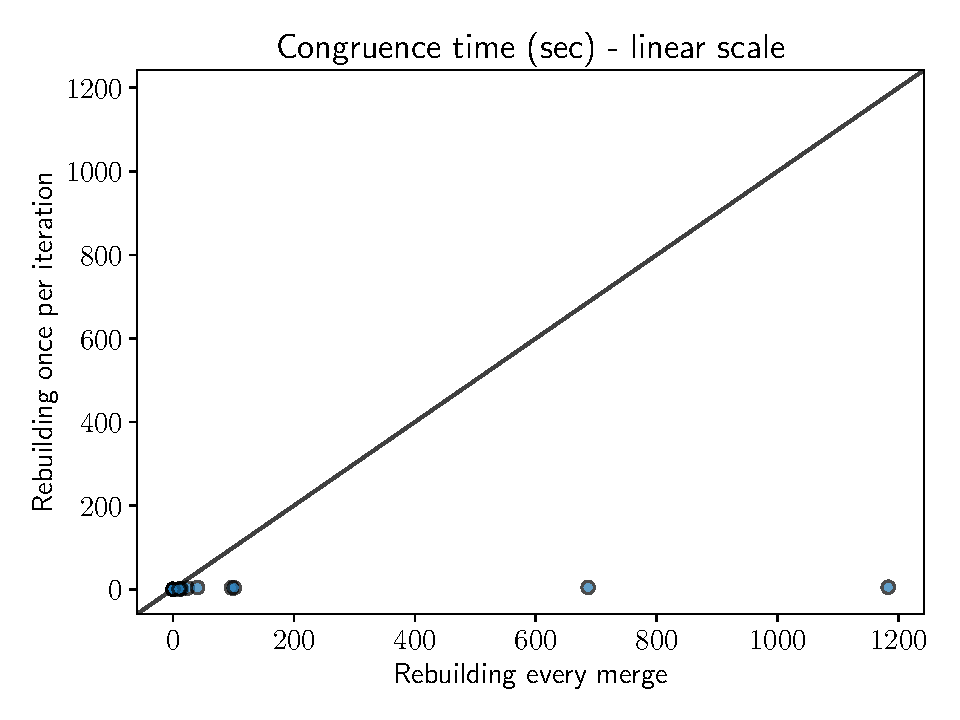
\includegraphics[width=\linewidth]{speedup}
  \end{subfigure}
  \hfill
  \begin{subfigure}{0.49\linewidth}
    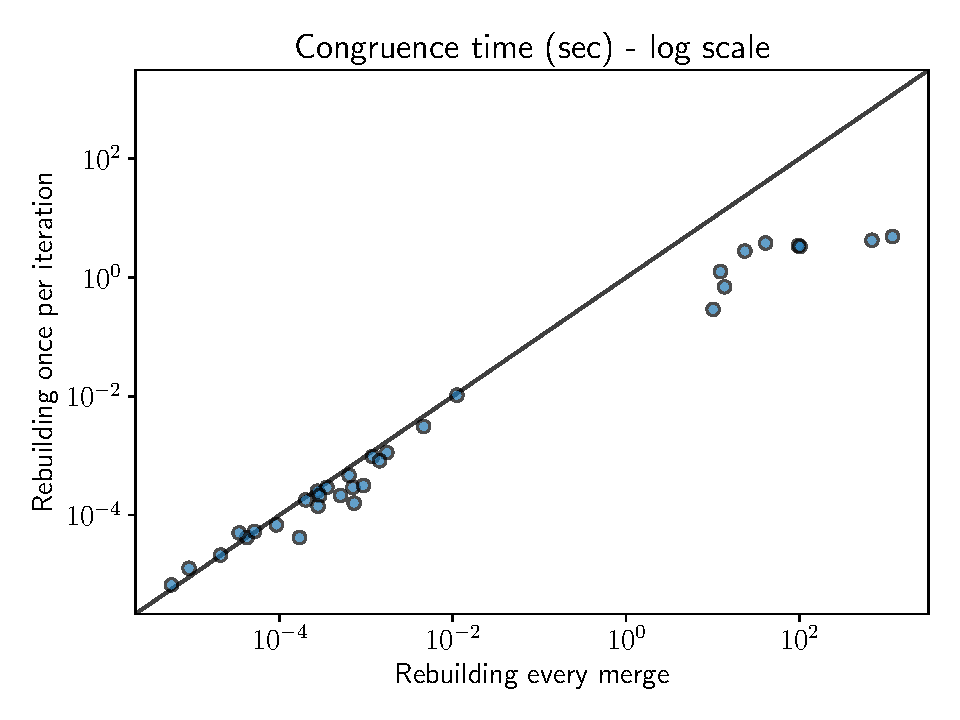
\includegraphics[width=\linewidth]{speedup-log}
  \end{subfigure}
  \caption{
    Rebuilding once per iteration---as opposed to after every merge---significantly
      speeds up congruence maintenance.
    Both plots show the same data: one point for each of the \nEggTests tests.
    The diagonal line is $y=x$;
      points below the line mean deferring rebuilding is faster.
    In aggregate over all tests (using geometric mean),
      congruence is \CongrSpeedup faster, and
      equality saturation is \TotalSpeedup faster.
    The linear scale plot shows that deferred rebuilding is significantly faster.
    The log scale plot suggests the speedup is greater than some constant multiple;
      \autoref{fig:eval-iter} demonstrates this in greater detail.
  }
  \label{fig:eval}

  \begin{minipage}[t]{0.48\linewidth}
  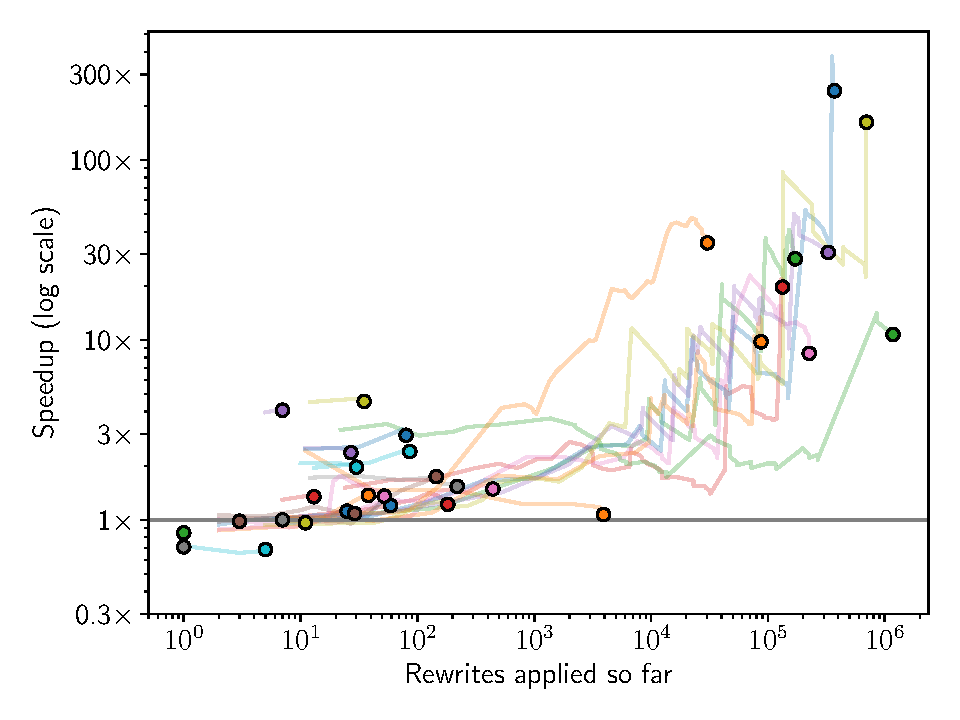
\includegraphics[width=\linewidth]{speedup-iter}
  \caption{
    As more rewrites are applied, deferring rebuilding gives greater speedup.
    Each line represents a single test: each equality saturation iteration plots
      the cumulative rewrites applied so far against the multiplicative speedup
      of deferring rebuilding; the dot represents the end of that test.
    Both the test suite as a whole (the dots) and individual tests (the lines)
      demonstrate an asymptotic speedup that increases with
      the problem size.
  }
  \label{fig:eval-iter}
  \end{minipage}
  \hfill
  \begin{minipage}[t]{0.48\linewidth}
  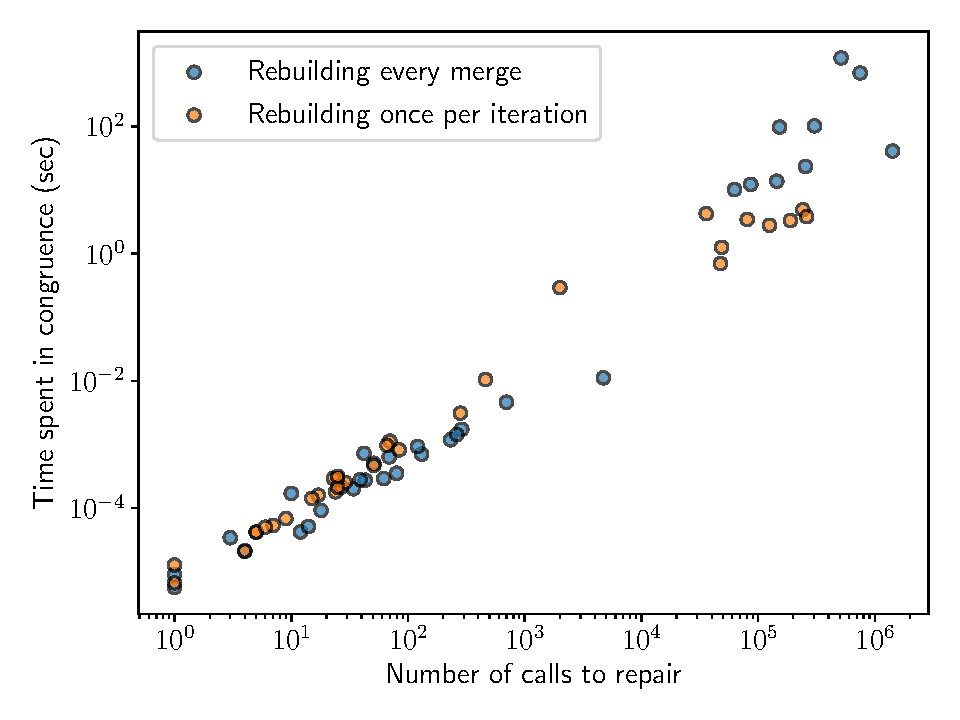
\includegraphics[width=\linewidth]{repairs}
  \caption{
    The time spent in congruence maintenance correlates with the number of calls
    to the \texttt{repair} method.
    Spearman correlation yields $r=\RepairsR$ with a p-value of \RepairsP,
    indicating that the two quantities are indeed positively correlated.
  }
  \label{fig:repair-plot}
  \end{minipage}
\end{figure}


We ran \egg's test suite using both rebuild strategies, measuring the time spent
  on congruence maintenance.
Each test consists of one run of \egg's equality saturation algorithm to optimize
  a given expression.
Of the \nEggTests total tests,
  \nEggTimeouts hit the iteration limit of 100 and the remainder saturated.
Note that both rebuilding strategies use \egg's phase-split equality saturation
  algorithm, and the resulting \egraphs are identical in all cases.
These experiments were performed on a 2020 Macbook Pro with a 2 GHz quad-core
  Intel Core i5 processor and 16GB of memory.

\autoref{fig:eval} shows our how rebuilding speeds up congruence maintenance.
Overall, our experiments show an aggregate \CongrSpeedup speedup on congruence
  closure and \TotalSpeedup speedup over the entire equality saturation
  algorithm.
\autoref{fig:eval-iter} shows this speedup is asymptotic;
  the multiplicative speedup increases as problem gets larger.

\egg's test suite consists of two main applications:
\texttt{math},
  a small computer algebra system capable of symbolic differentiation and
  integration; and
\texttt{lambda},
  a partial evaluator for the untyped lambda calculus using explicit
  substitution to handle variable binding (shown in \autoref{sec:impl}).
Both are typical \egg applications primarily driven by
  syntactic rewrites, with a few key uses of \egg's more complex features
  like \eclass analyses and dynamic/conditional rewrites.

\egg can be configured to capture various metrics about equality saturation as
  it runs, including the time spent in the read phase (searching for matches),
  the write phase (applying matches), and rebuilding.
In \autoref{fig:eval}, congruence time is measured as the time spent
  applying matches plus rebuilding.
Other parts of the equality saturation algorithm (creating the initial \egraph,
  extracting the final term) take negligible take compared to the equality
  saturation iterations.

Deferred rebuilding amortizes the examination of \eclasses
  for congruence maintenance;
  deduplicating the worklist reduces the number of calls to the \texttt{repair}.
\autoref{fig:repair-plot} shows that time spent in congruence is correlated with
  the number of calls to the \texttt{repair} methods.

The case study in \autoref{sec:herbie} provides a further evaluation of
  rebuilding. Rebuilding (and other \egg features) have also been implemented in
  a Racket-based \egraph, demonstrating that rebuilding is a conceptual advance
  that need not be tied to the \egg implementation.

%%% Local Variables:
%%% TeX-master: "../thesis"
%%% End:

\chapter{Extending \Egraphs with \Eclass Analyses}
\label{sec:extensions}

As discussed so far, \egraphs and equality saturation provide an efficient way
  to implement a term rewriting system.
Rebuilding enhances that efficiency, but the approach remains designed for
  purely syntactic rewrites.
However, program analysis and optimization typically require more than just
  syntactic information.
Instead, transformations are \emph{computed} based on the input terms and also semantic facts
  about that input term, e.g., constant value, free variables, nullability,
  numerical sign, size in memory, and so on.
The ``purely syntactic'' restriction has forced existing equality saturation
  applications~\cite{eqsat, eqsat-llvm, herbie} to
  resort to ad hoc passes over the \egraph
  to implement analyses like constant folding.
These ad hoc passes require manually manipulating the \egraph,
  the complexity of which could prevent the implementation of more sophisticated
  analyses.
  % naturally expressed in the more conventional term rewriting setting,
  % but must implemented as complicated \textit{ad hoc} passes over the \egraph.

We present a new technique called \textit{\eclass analysis},
  which allows the concise
  expression of a program analysis over the \egraph.
An \eclass analysis resembles abstract interpretation
  lifted to the \egraph level,
  attaching \textit{analysis data} from a semilattice to each \eclass.
The \egraph maintains and propagates this data as
  \eclasses get merged and new \enodes are added.
Analysis data can be used directly to modify the \egraph, to inform
  how or if rewrites apply their right-hand sides, or to determine the cost of
  terms during the extraction process.

\Eclass analyses provide a general mechanism to replace what previously
  required ad hoc extensions that manually manipulate the \egraph.
\Eclass analyses also fit within the equality saturation workflow,
  so they can naturally cooperate with the equational reasoning provided by
  rewrites.
Moreover, an analysis lifted to the \egraph level automatically benefits from a
  sort of ``partial-order reduction'' for free:
  large numbers of similar programs may be analyzed for little additional cost
  thanks to the \egraph's compact representation.

This section provides a conceptual explanation of \eclass analyses as well
  as dynamic and conditional rewrites that can use the analysis data.
The following sections will provide concrete examples:
  \autoref{sec:impl} discusses the \egg implementation and a complete example of a
  partial evaluator for the lambda calculus;
  \autoref{sec:case-studies} discusses how three published projects have used
  \egg and its unique features (like \eclass analyses).

% An \eclass analysis may,  modify the \egraph itself to inject new based on the computed data,
% In this way, the \eclass analysis can work with the rewrites as opposed

% \Egg offers many convenient ways to interact with the \egraph that are difficult
%   or impossible in other implementations.
% These tools give \egg the flexibility highlighted by the diverse case studies
%   in \autoref{sec:case-studies}
%   and the lambda calculus example in \autoref{sec:lambda}.

% Like the rest of \egg, these extensions are generic over the language and
%   rewrites that the user is working with.
% These are all novel in practice, as \egg is the first (to our knowledge)
%   general-purpose, reusable \egraph library.
% \Eclass analyses appear to be conceptually novel as well.

% \Chandra{this entire section is a bit light in details and doesn't
% always connect back to the goals of egg the right way. For example,
% without a concrete advantage of runners, it's not clear why it is useful.}

\section{E-Class Analyses}
\label{sec:analysis}

An \eclass analysis defines a domain $D$ and associates a value $d_{c} \in D$ to
  each \eclass $c$.
The \eclass $c$ contains the associated data $d_{c}$,
  i.e., given an \eclass $c$, one can get $d_{c}$ easily, but not vice-versa.

The interface of an \eclass analysis is as follows,
  where $G$ refers to the \egraph,
  and $n$ and $c$ refer to \enodes and \eclasses within $G$:

% We will use the following metavariables and syntax in this section:

% \begin{center}
%   $G$: \egraph, $c$: \eclass, $n$: \enode,
%   $d_{c}$: the analysis data associated with \eclass $c$
% \end{center}
\vspace{1em}
\begin{tabular}{lp{0.7\linewidth}}
  $\textsf{make}(n) \to d_{c}$ &
    When a new \enode $n$ is added to $G$ into a new, singleton \eclass $c$,
    construct a new value $d_{c} \in D$ to be associated with $n$'s new \eclass,
    typically by accessing the associated data of $n$'s children.
  \\
  $\textsf{join}(d_{c_1}, d_{c_2}) \to d_{c}$ &
    When \eclasses $c_{1}, c_{2}$ are being merged into $c$,
    join $d_{c_1}, d_{c_2}$ into a new value $d_{c}$ to be associated with the
    new \eclass $c$.
  \\
  $\textsf{modify}(c) \to c'$ &
    Optionally modify the \eclass $c$ based on $d_{c}$, typically by adding an
      \enode to $c$.
    Modify should be idempotent if no other changes occur to the \eclass, i.e.,
      $\textsf{modify}(\textsf{modify}(c)) = \textsf{modify}(c)$
    % Returning $c$ unmodified ($c = c'$) suffices in many cases, and is the
    % default implementation for analyses in \egg.
\end{tabular}
\vspace{1em}

The domain $D$ together with the \textsf{join} operation should form a join-semilattice.
The semilattice perspective is useful for defining the \textit{analysis invariant}
  (where $\wedge$ is the \textsf{join} operation):
\[
  \forall c \in G.\quad
  d_{c} = \bigwedge_{n \in c} \textsf{make}(n)
  \quad \text{and} \quad
  \textsf{modify}(c) = c
\]

The first part of the analysis invariant states that the data associated with
  each \eclass must be the \textsf{join} of the \textsf{make} for every \enode
  in that \eclass.
Since $D$ is a join-semilattice, this means that
  $\forall c, \forall n \in c, d_{c} \geq \textsf{make}(n) $.
The motivation for the second part is more subtle.
Since the analysis can modify an \eclass through the \textsf{modify} method,
  the analysis invariant asserts that these modifications are driven to a fixed
  point.
When the analysis invariant holds, a client looking at the analysis data can be
  assured that the analysis is ``stable'' in the sense that
  recomputing \textsf{make}, \textsf{join}, and \textsf{modify} will not
  modify the \egraph or any analysis data.

\subsection{Maintaining the Analysis Invariant}


\begin{figure}
  \begin{minipage}[t]{0.47\linewidth}
    \begin{lstlisting}[gobble=4, numbers=left, numberstyle=\color{black}, basicstyle=\scriptsize\ttfamily\color{black!40}, escapechar=|,
   xleftmargin=13pt,
   numbersep=7pt,
]
    def add(enode):
      enode = self.canonicalize(enode)
      if enode in self.hashcons:
        return self.hashcons[enode]
      else:
        eclass = self.new_singleton_eclass(enode)
        for child_eclass in enode.children:
          child_eclass.parents.add(enode, eclass)
        self.hashcons[enode] = eclass
        |\color{black}\label{line:add1} eclass.data = analysis.make(enode)|
        |\color{black}\label{line:add2} analysis.modify(eclass)|
        return eclass

    def merge(eclass1, eclass2)
      union = self.union_find.union(eclass1, eclass2)
      if not union.was_already_unioned:
        |\color{black}\label{line:merge1}d1, d2 = eclass1.data, eclass2.data|
        |\color{black}\label{line:merge2}union.eclass.data = analysis.join(d1, d2)|
        self.worklist.add(union.eclass)
      return union.eclass
    \end{lstlisting}
  \end{minipage}
  \hfill
  \begin{minipage}[t]{0.47\linewidth}
    \begin{lstlisting}[gobble=4, numbers=left, firstnumber=21, numberstyle=\color{black}, basicstyle=\scriptsize\ttfamily\color{black!40}, escapechar=|,
    numbersep=5pt,
]
    def repair(eclass):
      for (p_node, p_eclass) in eclass.parents:
        self.hashcons.remove(p_node)
        p_node = self.canonicalize(p_node)
        self.hashcons[p_node] = self.find(p_eclass)

      new_parents = {}
      for (p_node, p_eclass) in eclass.parents:
        p_node = self.canonicalize(p_node)
        if p_node in new_parents:
          self.union(p_eclass, new_parents[p_node])
        new_parents[p_node] = self.find(p_eclass)
      eclass.parents = new_parents
    \end{lstlisting}
    \vspace{-3mm}
    \begin{lstlisting}[gobble=4, numbers=left, firstnumber=34, basicstyle=\scriptsize\ttfamily, escapechar=|,
    numbersep=5pt,
]

      # any mutations modify makes to eclass
      # will add to the worklist
      |\label{line:repair1}|analysis.modify(eclass)
      for (p_node, p_eclass) in eclass.parents:
        new_data = analysis.join(
          p_eclass.data,
          analysis.make(p_node))
        if new_data != p_eclass.data:
          p_eclass.data = new_data
          |\label{line:repair2}|self.worklist.add(p_eclass)
    \end{lstlisting}
  \end{minipage}
  \caption{
    The pseudocode for maintaining the \eclass analysis invariant is largely
      similar to how rebuilding maintains congruence closure
      (\autoref{sec:rebuilding}).
    Only lines \ref{line:add1}--\ref{line:add2},
      \ref{line:merge1}--\ref{line:merge2},
      and \ref{line:repair1}--\ref{line:repair2} are added.
    Grayed out or missing code is unchanged from \autoref{fig:rebuild-code}.
  }
  \label{fig:rebuild-analysis}
\end{figure}

We extend the rebuilding procedure from \autoref{sec:rebuilding} to restore the
  analysis invariant as well as the congruence invariant.
\autoref{fig:rebuild-analysis} shows the necessary modifications to the
  rebuilding code from \autoref{fig:rebuild-code}.

Adding \enodes and merging \eclasses risk breaking the analysis invariant in
  different ways.
Adding \enodes is the simpler case; lines \ref{line:add1}--\ref{line:add2}
  restore the invariant for the newly created, singleton \eclass that holds the
  new \enode.
When merging \enodes, the first concern is maintaining the semilattice portion of the
  analysis invariant.
Since \textsf{join} forms a semilattice over the domain $D$ of the analysis
  data, the order in which the joins occur does not matter.
Therefore, line \ref{line:merge2} suffices to update the analysis data of the
  merged \eclass.

Since $\textsf{make}(n)$ creates analysis data by looking at the data of $n$'s,
  children, merging \eclasses can violate the analysis invariant in the same way
  it can violate the congruence invariant.
The solution is to use the same worklist mechanism introduced in
  \autoref{sec:rebuilding}.
Lines \ref{line:repair1}--\ref{line:repair2} of the \texttt{repair} method
  (which \texttt{rebuild} on each element of the worklist)
  re-\textsf{make} and \textsf{merge} the analysis data of the parent of any
  recently merged \eclasses.
The new \texttt{repair} method also calls \textsf{modify} once, which suffices
  due to its idempotence.
In the pseudocode, \textsf{modify} is reframed as a mutating method for clarity.

\Egg's implementation of \eclass analyses assumes that the analysis domain $D$
  is indeed a semilattice and that \textsf{modify} is idempotent.
Without these properties, \egg may fail to restore the analysis invariant on
  \texttt{rebuild}, or it may not terminate.

% \subsection{Modifying the \Egraph from an \Eclass Analysis}
\subsection{Example: Constant Folding}

The data produced by \eclass analyses can be
  usefully consumed by other components of an equality saturation system
  (see \autoref{sec:rewrites}),
  but \eclass analyses can be useful on their own thanks to the
  \textsf{modify} hook.
Typical \textsf{modify} hooks will either do nothing, check some invariant about
  the \eclasses being merged, or add an \enode to that \eclass
  (using the regular \texttt{add} and \texttt{merge} methods of the \egraph).

As mentioned above, other equality saturation implementations have implemented
  constant folding as custom, ad hoc passes over the \egraph.
We can formulate constant folding as an \eclass analysis that highlights the
  parallels with abstract interpretation.
Let the domain $D = \texttt{Option<Constant>}$, and let the \texttt{join}
  operation be the ``\texttt{or}'' operation of the \texttt{Option} type:
\begin{figure}[h!]
\begin{lstlisting}[language=Rust, basicstyle=\ttfamily\footnotesize, xleftmargin=35mm]
match (a, b) {
  (None,    None   ) => None,
  (Some(x), None   ) => Some(x),
  (None,    Some(y)) => Some(y),
  (Some(x), Some(y)) => { assert!(x == y); Some(x) }
}
\end{lstlisting}
\end{figure}
Note how \textsf{join} can also aid in debugging by checking properties about
  values that are unified in the \egraph;
  in this case we assert that all terms represented in an \eclass should have
  the same constant value.
The \textsf{make} operation serves as the abstraction function, returning the
  constant value of an \enode if it can be computed from the constant values
  associated with its children \eclasses.
The \textsf{modify} operation serves as a concretization function in this
  setting.
If $d_{c}$ is a constant value, then $\textsf{modify}(c)$ would add
  $\gamma(d_{c}) = n$ to $c$, where $\gamma$ concretizes the constant value into
  a childless \enode.

Constant folding is an admittedly simple analysis, but one that did not formerly
  fit within the equality saturation framework.
\Eclass analyses support more complicated analyses in a general way, as
  discussed in later sections on the \egg implementation and case studies
  (Sections \ref{sec:impl} and \ref{sec:case-studies}).

\section{Conditional and Dynamic Rewrites}
\label{sec:rewrites}

In equality saturation applications, most of the rewrites are purely
  syntactic.
In some cases, additional data may be needed to determine if or how to perform
  the rewrite.
For example, the rewrite $x / x \to 1$ is only valid if $x \neq 0$.
A more complex rewrite may need to compute the right-hand side dynamically based
  on an analysis fact from the left-hand side.

The right-hand side of a rewrite can be generalized to a function
  \textsf{apply} that takes a substitution and an \eclass generated from
  e-matching the left-hand side, and produces a term to be added to the \egraph
  and unified with the matched \eclass.
For a purely syntactic rewrite, the \textsf{apply} function need not inspect the
  matched \eclass in any way; it would simply apply
  the substitution to the right-hand pattern to produce a new term.

\Eclass analyses greatly increase the utility of this generalized form of
  rewriting.
The \textsf{apply} function can look at the analysis data for the matched
  \eclass or any of the \eclasses in the substitution to determine if or how to
  construct the right-hand side term.
These kinds of rewrites can broken down further into two categories:
\begin{itemize}
  \item \textit{Conditional} rewrites like $x / x \to 1$ that are purely
  syntactic but whose validity depends on checking some analysis data;
  \item \textit{Dynamic} rewrites that compute the right-hand side based on
  analysis data.
\end{itemize}

Conditional rewrites are a subset of the more general dynamic rewrites.
Our \egg implementation supports both.
The example in \autoref{sec:impl} and case studies in \autoref{sec:case-studies}
  heavily use generalized rewrites, as it is typically the most convenient way
  to incorporate domain knowledge into the equality saturation
  framework.

\section{Extraction}
\label{sec:tricks-extraction}

Equality saturation typically ends with an extraction phase that selects an
  optimal represented term from an \eclass according to some cost function.
In many domains \cite{herbie, szalinski}, AST size
  (sometimes weighted differently for different operators) suffices as a simple,
  local cost function.
We say a cost function $k$ is local when the cost of a term $f(a_{1}, ...)$ can be
  computed from the function symbol $f$ and the costs of the children.
With such cost functions, extracting an optimal term can be efficiently done
  with a fixed-point traversal over the \egraph that selects the minimum cost
  \enode from each \eclass \cite{herbie}.

Extraction can be formulated as an \eclass analysis when the cost function
  is local.
The analysis data is a tuple $(n, k(n))$ where $n$ is the cheapest \enode
  in that \eclass and $k(n)$ its cost.
The $\textsf{make}(n)$ operation calculates the cost $k(n)$ based on
  the analysis data (which contain the minimum costs) of $n$'s children.
The \textsf{merge} operation simply takes the tuple with lower cost.
The semilattice portion of the analysis invariant then guarantees that the
  analysis data will contain the lowest-cost \enode in each class.
Extract can then proceed recursively;
  if the analysis data for \eclass $c$ gives $f(c_{1}, c_{2}, ...)$ as the optimal \enode,
  the optimal term represented in $c$ is
  $\textsf{extract}(c) = f( \textsf{extract}(c_{1}), \textsf{extract}(c_{2}), ... )$.
% The optimal term represented in an \eclass can then be built recursively,
%   starting with the optimal \enode from the analysis data.
% Extraction can be completed by starting from the desired \eclass and
%   building the term recursively based on the \enode from the analysis data.
This not only further demonstrates the generality of \eclass analyses, but also
  provides the ability to do extraction ``on the fly''; conditional and dynamic
  rewrites can determine their behavior based on the cheapest term in an \eclass.

Extraction (whether done as a separate pass or an \eclass analysis) can also
  benefit from the analysis data.
Typically, a local cost function can only look at the function symbol of the
  \enode $n$ and the costs of $n$'s children.
When an \eclass analysis is attached to the \egraph, however, a cost function
  may observe the data associated with $n$'s \eclass, as well as the data
  associated with $n$'s children.
This allows a cost function to depend on computed facts rather that just purely
  syntactic information.
In other words, the cost of an operator may differ based on its inputs.
\autoref{sec:spores} provides a motivating case study wherein an \eclass
  analysis computes the size and shape of tensors, and this size information
  informs the cost function.

%%% Local Variables:
%%% TeX-master: "../thesis"
%%% End:

\chapter{\egg: Easy, Extensible, and Efficient \Egraphs}

\label{sec:egg}
\label{sec:impl}
\label{sec:lambda}

We implemented the techniques of rebuilding and \eclass analysis in \egg,
  an easy-to-use, extensible, and efficient \egraph library.
To the best of our knowledge,
  \egg is the first general-purpose, reusable \egraph implementation.
This has allowed focused effort on ease of use and optimization,
  knowing that any benefits will
  be seen across use cases as opposed to a single, ad hoc instance.

This section details \egg's implementation and some of the various
  optimizations and tools it provides to the user.
We use an extended example of a partial evaluator for the lambda calculus\footnote{
  \Egraphs do not have any ``built-in'' support for binding;
  for example, equality modulo alpha renaming is not free.
  The explicit substitution provided in this section is is illustrative but rather high in performance cost.
  Better support for languages with binding is important future work.
},
  for which we provide the complete source code (which few changes for readability)
  in \autoref{fig:lambda-lang} and \autoref{fig:lambda-analysis}.
While contrived, this example is compact and familiar, and it highlights
  (1) how \egg is used and (2) some of its novel features like
  \eclass analyses and dynamic rewrites.
It demonstrates how \egg can tackle binding,
  a perennially tough problem for \egraphs,
  with a simple explicit substitution approach
  powered by \egg's extensibility.
\autoref{sec:case-studies} goes further, providing real-world case studies of
  published projects that have depended on \egg.

\egg is implemented in \textasciitilde{}5000 lines of Rust,\footnote
{
  Rust \cite{rust} is a high-level systems programming language.
  \egg has been integrated into applications written in other
  programming languages using both C FFI and serialization approaches.
}
including code, tests, and documentation.
\egg is open-source, well-documented, and distributed via Rust's package
  management system.\footnote{
  Source: \url{https://github.com/mwillsey/egg}.
  Documentation: \url{https://docs.rs/egg}.
  Package: \url{https://crates.io/crates/egg}.
  \\
  This paper uses version 0.6 of \egg.
}
All of \egg's components are generic over the
  user-provided language, analysis, and cost functions.

\section{Ease of Use}
\label{sec:egg-easy}

\begin{figure}
\begin{subfigure}[t]{0.48\linewidth}
  \begin{lstlisting}[language=Rust, basicstyle=\tiny\ttfamily, numbers=left, escapechar=|,
   xleftmargin=13pt,
   numbersep=7pt,
]
define_language! {
  enum Lambda {
    // enum variants have data or children (eclass Ids)
    // [Id; N] is an array of N `Id`s

    // base type operators
    "+" = Add([Id; 2]), "=" = Eq([Id; 2]),
    "if" = If([Id; 3]),

    // functions and binding
    "app" = App([Id; 2]), "lam" = Lambda([Id; 2]),
    "let" = Let([Id; 3]), "fix" = Fix([Id; 2]),

    // (var x) is a use of `x` as an expression
    "var" = Use(Id),
    // (subst a x b) substitutes a for (var x) in b
    "subst" = Subst([Id; 3]),

    // base types have no children, only data
    Bool(bool), Num(i32), Symbol(String),
  }
}

// example terms and what they simplify to
// pulled directly from the |\egg|test suite

test_fn! { lambda_under, rules(),
  "(lam x (+ 4 (app (lam y (var y)) 4)))"
  => "(lam x 8))",
}

test_fn! { lambda_compose_many, rules(),
  "(let compose (lam f (lam g (lam x
                (app (var f)
                     (app (var g) (var x))))))
   (let add1 (lam y (+ (var y) 1))
   (app (app (var compose) (var add1))
        (app (app (var compose) (var add1))
             (app (app (var compose) (var add1))
                  (app (app (var compose) (var add1))
                       (var add1)))))))"
  => "(lam ?x (+ (var ?x) 5))"
}

test_fn! { lambda_if_elim, rules(),
  "(if (= (var a) (var b))
       (+ (var a) (var a))
       (+ (var a) (var b)))"
  => "(+ (var a) (var b))"
}\end{lstlisting}
\end{subfigure}
\hfill
\begin{subfigure}[t]{0.48\linewidth}
  \begin{lstlisting}[language=Rust, basicstyle=\tiny\ttfamily, escapechar=|, numbers=left, firstnumber=51,
  numbersep=7pt,
]
// Returns a list of rewrite rules
fn rules() -> Vec<Rewrite<Lambda, LambdaAnalysis>> { vec![

 // open term rules
 rw!("if-true";  "(if  true ?then ?else)" => "?then"),
 rw!("if-false"; "(if false ?then ?else)" => "?else"),
 rw!("if-elim";  "(if (= (var ?x) ?e) ?then ?else)" => "?else"
     if ConditionEqual::parse("(let ?x ?e ?then)",
                              "(let ?x ?e ?else)")),
 rw!("add-comm";  "(+ ?a ?b)"        => "(+ ?b ?a)"),
 rw!("add-assoc"; "(+ (+ ?a ?b) ?c)" => "(+ ?a (+ ?b ?c))"),
 rw!("eq-comm";   "(= ?a ?b)"        => "(= ?b ?a)"),

 // substitution introduction
 rw!("fix";     "(fix ?v ?e)" =>
                "(let ?v (fix ?v ?e) ?e)"),
 rw!("beta";    "(app (lam ?v ?body) ?e)" =>
                "(let ?v ?e ?body)"),

 // substitution propagation
 rw!("let-app"; "(let ?v ?e (app ?a ?b))" =>
                "(app (let ?v ?e ?a) (let ?v ?e ?b))"),
 rw!("let-add"; "(let ?v ?e (+   ?a ?b))" =>
                "(+   (let ?v ?e ?a) (let ?v ?e ?b))"),
 rw!("let-eq";  "(let ?v ?e (=   ?a ?b))" =>
                "(=   (let ?v ?e ?a) (let ?v ?e ?b))"),
 rw!("let-if";  "(let ?v ?e (if ?cond ?then ?else))" =>
                "(if (let ?v ?e ?cond)
                     (let ?v ?e ?then)
                     (let ?v ?e ?else))"),

 // substitution elimination
 rw!("let-const";    "(let ?v ?e ?c)" => "?c"
     if is_const(var("?c"))),
 rw!("let-var-same"; "(let ?v1 ?e (var ?v1))" => "?e"),
 rw!("let-var-diff"; "(let ?v1 ?e (var ?v2))" => "(var ?v2)"
     if is_not_same_var(var("?v1"), var("?v2"))),
 rw!("let-lam-same"; "(let ?v1 ?e (lam ?v1 ?body))" =>
                     "(lam ?v1 ?body)"),
 rw!("let-lam-diff"; "(let ?v1 ?e (lam ?v2 ?body))" =>
     ( CaptureAvoid {
        fresh: var("?fresh"), v2: var("?v2"), e: var("?e"),
        if_not_free: "(lam ?v2 (let ?v1 ?e ?body))"
                     .parse().unwrap(),
        if_free: "(lam ?fresh (let ?v1 ?e
                              (let ?v2 (var ?fresh) ?body)))"
                 .parse().unwrap(),
     })
     if is_not_same_var(var("?v1"), var("?v2"))),
]}\end{lstlisting}
\end{subfigure}
\vspace{-0.5em}
\caption[Language and rewrites for the lambda calculus in \egg]{
\egg is generic over user-defined languages;
  here we define a language and rewrite rules for a lambda calculus partial evaluator.
The provided \texttt{define\_language!} macro (lines 1-22) allows the simple definition
  of a language as a Rust \texttt{enum}, automatically deriving parsing and
  pretty printing.
A value of type \texttt{Lambda} is an \enode that holds either data that the
  user can inspect or some number of \eclass children (\eclass \texttt{Id}s).

Rewrite rules can also be defined succinctly (lines 51-100).
Patterns are parsed as s-expressions:
  strings from the \texttt{define\_language!} invocation (ex: \texttt{fix}, \texttt{=}, \texttt{+}) and
  data from the variants (ex: \texttt{false}, \texttt{1}) parse as operators or terms;
  names prefixed by ``\texttt{?}'' parse as pattern variables.

Some of the rewrites made are conditional using the
  ``\texttt{left => right if cond}''
  syntax.
The \texttt{if-elim} rewrite on line 57 uses \egg's provided
  \texttt{ConditionEqual} as a condition, only applying the right-hand side
  if the \egraph can prove the two argument patterns equivalent.
The final rewrite, \texttt{let-lam-diff}, is dynamic to support capture avoidance;
  the right-hand side is a Rust value that
  implements the \texttt{Applier} trait instead of a pattern.
\autoref{fig:lambda-analysis} contains the supporting code for these rewrites.

We also show some of the tests (lines 27-50)
  from \egg's \texttt{lambda} test suite.
The tests proceed by inserting the term on the left-hand side, running
  \egg's equality saturation, and then checking to make sure the right-hand
  pattern can be found in the same \eclass as the initial term.
}
\label{fig:lambda-rules}
\label{fig:lambda-lang}
\label{fig:lambda-examples}
\end{figure}

%%% Local Variables:
%%% TeX-master: "../thesis"
%%% End:


\egg's ease of use comes primarily from its design as a library.
By defining only a language and some rewrite rules,
  a user can quickly
  start developing a synthesis or optimization tool.
Using \egg as a Rust library,
  the user defines the language using the \texttt{define\_language!} macro
  shown in \autoref{fig:lambda-lang}, lines 1-22.
Childless variants in the language may contain data of user-defined types,
  and \eclass analyses or dynamic rewrites may inspect this data.

%Defining a language is the only necessary input for \egg.
%From there, a user may create and manipulate \egraphs that hold expressions from
%  that language.
%If the user wants to perform rewrites and equality saturation, \egg provides
%  facilities for this as well.

The user provides rewrites as shown in
  \autoref{fig:lambda-lang}, lines 51-100.
Each rewrite has a name, a left-hand side, and a right-hand side.
For purely syntactic rewrites, the right-hand is simply a pattern.
More complex rewrites can incorporate conditions or even dynamic right-hand
  sides, both explained in the \autoref{sec:egg-extensible} and \autoref{fig:lambda-applier}.

Equality saturation workflows, regardless of the application domain,
  typically have a similar structure:
add expressions to an empty \egraph, run rewrites until saturation or
  timeout, and extract the best equivalent expressions according to some cost
  function.
This ``outer loop'' of equality saturation involves a significant amount of
  error-prone boilerplate:
\begin{itemize}
  \item Checking for saturation, timeouts, and \egraph size limits.
  \item Orchestrating the read-phase, write-phase, rebuild system
    (\autoref{fig:rebuild-code}) that makes \egg fast.
  \item Recording performance data at each iteration.
  \item Potentially coordinating rule execution so that expansive rules like
    associativity do not dominate the \egraph.
  \item Finally, extracting the best expression(s) according to a
  user-defined cost function.
\end{itemize}

\egg provides these functionalities through its \texttt{Runner} and
  \texttt{Extractor} interfaces.
\texttt{Runner}s automatically detect saturation, and can be configured to stop
  after a time, \egraph size, or iterations limit.
The equality saturation loop provided by \egg calls \texttt{rebuild}, so users
  need not even know about \egg's deferred invariant maintenance.
\texttt{Runner}s record various metrics about each iteration automatically,
  and the user can hook into this to report relevant data.
\texttt{Extractor}s select the optimal term from an \egraph given a
  user-defined, local cost function.\footnote{
    As mentioned in \autoref{sec:tricks-extraction}, extraction can be
    implemented as part of an \eclass analysis.
    The separate \texttt{Extractor} feature is still useful for ergonomic and
    performance reasons.
  }
The two can be combined as well; users commonly record the ``best so far''
  expression by extracting in each iteration.

\autoref{fig:lambda-lang} also shows \egg's \texttt{test\_fn!}
  macro for easily creating tests (lines 27-50).
These tests create an \egraph with the given expression, run equality saturation
  using a \texttt{Runner}, and check to make sure the right-hand pattern can be
  found in the same \eclass as the initial expression.

\section{Extensibility}
\label{sec:egg-extensible}

For simple domains, defining a language and purely syntactic rewrites will
  suffice.
However, our partial evaluator requires interpreted reasoning, so we use some of
  \egg's more advanced features like \eclass analyses and dynamic rewrites.
Importantly, \egg supports these extensibility features as a library:
  the user need not modify the \egraph or \egg's internals.

\begin{figure}
\begin{minipage}[t]{0.49\linewidth}
  \begin{lstlisting}[
   language=Rust, basicstyle=\tiny\ttfamily, numbers=left,
   xleftmargin=11pt,
   numbersep=5pt,
]
type EGraph = egg::EGraph<Lambda, LambdaAnalysis>;
struct LambdaAnalysis;
struct FC {
  free: HashSet<Id>,    // our analysis data stores free vars
  constant: Option<Lambda>, // and the constant value, if any
}

// helper function to make pattern meta-variables
fn var(s: &str) -> Var { s.parse().unwrap() }

impl Analysis<Lambda> for LambdaAnalysis {
  type Data = FC; // attach an FC to each eclass
  // merge implements semilattice join by joining into `to`
  // returning true if the `to` data was modified
  fn merge(&self, to: &mut FC, from: FC) -> bool {
    let before_len = to.free.len();
    // union the free variables
    to.free.extend(from.free.iter().copied());
    if to.constant.is_none() && from.constant.is_some() {
      to.constant = from.constant;
      true
    } else {
      before_len != to.free.len()
    }
  }

  fn make(egraph: &EGraph, enode: &Lambda) -> FC {
    let f = |i: &Id| egraph[*i].data.free.iter().copied();
    let mut free = HashSet::default();
    match enode {
      Use(v) => { free.insert(*v); }
      Let([v, a, b]) => {
        free.extend(f(b)); free.remove(v); free.extend(f(a));
      }
      Lambda([v, b]) | Fix([v, b]) => {
        free.extend(f(b)); free.remove(v);
      }
      _ => enode.for_each_child(
             |c| free.extend(&egraph[c].data.free)),
    }
    FC { free: free, constant: eval(egraph, enode) }
  }

  fn modify(egraph: &mut EGraph, id: Id) {
    if let Some(c) = egraph[id].data.constant.clone() {
      let const_id = egraph.add(c);
      egraph.union(id, const_id);
    }
  }
}\end{lstlisting}
\end{minipage}
\hfill
\begin{minipage}[t]{0.46\linewidth}
  \begin{lstlisting}[language=Rust, basicstyle=\tiny\ttfamily, escapechar=@, numbers=left, firstnumber=51,
   numbersep=7pt,
]
// evaluate an enode if the children have constants
// Rust's `?` extracts an Option, early returning if None
fn eval(eg: &EGraph, enode: &Lambda) -> Option<Lambda> {
  let c = |i: &Id| eg[*i].data.constant.clone();
  match enode {
    Num(_) | Bool(_) => Some(enode.clone()),
    Add([x, y]) => Some(Num(c(x)? + c(y)?)),
    Eq([x, y]) => Some(Bool(c(x)? == c(y)?)),
    _ => None,
  }
}

// Functions of this type can be conditions for rewrites
trait ConditionFn = Fn(&mut EGraph, Id, &Subst) -> bool;

// The following two functions return closures of the
// correct signature to be used as conditions in @\autoref{fig:lambda-rules}@.
fn is_not_same_var(v1: Var, v2: Var) -> impl ConditionFn {
    |eg, _, subst| eg.find(subst[v1]) != eg.find(subst[v2])
}
fn is_const(v: Var) -> impl ConditionFn {
     // check the LambdaAnalysis data
    |eg, _, subst| eg[subst[v]].data.constant.is_some()
}

struct CaptureAvoid {
  fresh: Var, v2: Var, e: Var,
  if_not_free: Pattern<Lambda>, if_free: Pattern<Lambda>,
}

impl Applier<Lambda, LambdaAnalysis> for CaptureAvoid {
  // Given the egraph, the matching eclass id, and the
  // substitution generated by the match, apply the rewrite
  fn apply_one(&self, egraph: &mut EGraph,
               id: Id, subst: &Subst) -> Vec<Id>
  {
    let (v2, e) = (subst[self.v2], subst[self.e]);
    let v2_free_in_e = egraph[e].data.free.contains(&v2);
    if v2_free_in_e {
      let mut subst = subst.clone();
      // make a fresh symbol using the eclass id
      let sym = Lambda::Symbol(format!("_{}", id).into());
      subst.insert(self.fresh, egraph.add(sym));
      // apply the given pattern with the modified subst
      self.if_free.apply_one(egraph, id, &subst)
    } else {
      self.if_not_free.apply_one(egraph, id, &subst)
    }
  }
}\end{lstlisting}
  % \caption{
  %   Some of the rewrites in \autoref{fig:lambda-rules} are conditional,
  %     requiring conditions like \texttt{is\_not\_same\_var} or \texttt{is\_const}.
  %   Others are fully dynamic, using a custom applier like \texttt{CaptureAvoid}
  %     instead of a syntactic right-hand side.
  %   Both conditions and custom appliers can use the computed data from the
  %     \eclass analysis; for example, \texttt{CaptureAvoid} only $\alpha$-renames if
  %     there might be a name collision.
  % }
\end{minipage}
\caption[\Eclass analysis and conditional/dynamic rewrites for the lambda calculus]{
Our partial evaluator example highlights three important features \egg provides
  for extensibility: \eclass analyses, conditional rewrites, and dynamic
  rewrites.
  
The \texttt{LambdaAnalysis} type, which implements the \texttt{Analysis} trait,
  represents the \eclass analysis.
Its associated data (\texttt{FC}) stores
  the constant term from that \eclass (if any) and
  an over-approximation of the free variables used by terms in that \eclass.
The constant term is used to perform constant folding.
The \texttt{merge} operation implements the semilattice join, combining the free
  variable sets and taking a constant if one exists.
In \texttt{make}, the analysis computes the free variable sets based on the
  \enode and the free variables of its children;
  the \texttt{eval} generates the new constants if possible.
The \texttt{modify} hook of \texttt{Analysis} adds the constant to the \egraph.

Some of the conditional rewrites in \autoref{fig:lambda-rules} depend on
  conditions defined here.
Any function with the correct signature may serve as a condition.

The \texttt{CaptureAvoid} type implements the \texttt{Applier} trait, allowing
  it to serve as the right-hand side of a rewrite.
\texttt{CaptureAvoid} takes two patterns and some pattern variables.
It checks the free variable set to determine if a capture-avoiding substitution
  is required, applying the \texttt{if\_free} pattern if so and the
  \texttt{if\_not\_free} pattern otherwise.
}
\label{fig:lambda-applier}
\label{fig:lambda-analysis}
\end{figure}

%%% Local Variables:
%%% TeX-master: "../thesis"
%%% End:


\autoref{fig:lambda-applier} shows the remainder of the code for our lambda
  calculus partial evaluator.
It uses an \eclass analysis (\texttt{LambdaAnalysis})
  to track free variables and constants associated
  with each \eclass.
The implementation of the \eclass analysis is in Lines 11-50.
The \eclass analysis invariant
  guarantees that the analysis data contains an over-approximation of free variables
  from terms represented in that \eclass.
The analysis also does constant folding
  (see the \texttt{make} and \texttt{modify} methods).
The \texttt{let-lam-diff} rewrite (Line 90, \autoref{fig:lambda-rules})
  uses the \texttt{CaptureAvoid} (Lines 81-100, \autoref{fig:lambda-applier})
  dynamic right-hand side to do capture-avoiding
  substitution only when necessary based on the free variable information.
The conditional rewrites from \autoref{fig:lambda-rules} depend on the
  conditions \texttt{is\_not\_same\_var} and
  \texttt{is\_var} (Lines 68-74, \autoref{fig:lambda-applier})
  to ensure correct substitution.

\egg is extensible in other ways as well.
As mentioned above, \texttt{Extractor}s are parameterized by a user-provided
  cost function.
\texttt{Runner}s are also extensible with user-provided rule schedulers that can
  control the behavior of potentially troublesome rewrites.
\label{sec:rule-scheduling}
In typical equality saturation, each rewrite is searched for and applied each
  iteration.
This can cause certain rewrites, commonly associativity or distributivity,
  to dominate others and make the search space less productive.
Applied in moderation, these rewrites can trigger other rewrites and find
  greatly improved expressions,
  but they can also slow the search by
  exploding the \egraph exponentially in size.
By default, \egg uses the built-in backoff scheduler
  that identifies rewrites that are matching in exponentially-growing
  locations and temporarily bans them.
We have observed that this greatly reduced run time (producing the same results)
  in many settings.
\egg can also use a conventional every-rule-every-time scheduler, or the user
  can supply their own.

\section{Efficiency}
\label{sec:egg-efficient}

\egg's novel \textit{rebuilding} algorithm (\autoref{sec:rebuild})
combined with systems programming best practices
  makes \egraphs---and the equality saturation
  use case in particular---more efficient than prior tools.

\egg is implemented in Rust, giving the compiler freedom to
  specialize and inline user-written code.
This is especially important as
  \egg's generic nature leads to tight interaction
  between library code
  (e.g., searching for rewrites) and user code (e.g., comparing operators).
\egg is designed from the ground up to use cache-friendly,
  flat buffers with minimal indirection for most internal data structures.
This is in sharp contrast to traditional representations of \egraphs
  \cite{nelson, simplify} that contains many tree- and linked list-like data
  structures.
\egg additionally compiles patterns to be executed by a small virtual machine
  \cite{ematching}, as opposed to recursively walking the tree-like
  representation of patterns.

Aside from deferred rebuilding, \egg's equality saturation algorithm leads to
  implementation-level performance enhancements.
Searching for rewrite matches, which is the bulk of running time, can be
  parallelized thanks to the phase separation.
Either the rules or \eclasses could be searched in parallel.
Furthermore, the once-per-iteration frequency of rebuilding allows \egg to
  establish other performance-enhancing invariants that hold during the
  read-only search phase.
For example, \egg sorts \enodes within each \eclass to enable binary search, and
  also maintains a cache mapping function symbols to \eclasses that
  contain \enodes with that function symbol.

Many of \egg's extensibility features can also be used to improve performance.
As mentioned above, rule scheduling can lead to great performance improvement in
  the face of ``expansive'' rules that would otherwise dominate the search
  space.
The \texttt{Runner} interface also supports user hooks that can stop
  the equality saturation after some arbitrary condition.
This can be useful when using equality saturation to prove terms equal; once
  they are unified, there is no point in continuing.
\label{sec:egg-batched}
\egg's \texttt{Runner}s also support batch simplification, where multiple terms
  can be added to the initial \egraph before running equality saturation.
If the terms are substantially similar, both rewriting and any \eclass analyses
  will benefit from the \egraph's inherent structural deduplication.
The case study in \autoref{sec:herbie} uses batch simplification to achieve
  a large speedup with simplifying similar expressions.

%%% Local Variables:
%%% TeX-master: "../thesis"
%%% End:

\chapter{Case Studies}
\label{sec:case-studies}

This thesis makes the case that equality saturation
 (and \egg in particular)
 is the right tool for
 many program optimization and synthesis tasks.
The preceding chapters have articulated the
 technical novelties, practical features,
 and quantitative evidence that supports this claim.
This chapter provides qualitative evidence through case studies
 of independently-developed
 projects\footnotemark{}
 from diverse domains
 that incorporated \egg.

Users have built program synthesizers, optimizers, and provers
 with \egg across domains such as
 floating point accuracy, 3D CAD, deep learning, mutation testing,
 automatic vectorization, and more.
In many cases, the developers had first rolled their own \egraph
 implementations;
 \egg allowed them to delete code, gain performance, and in some cases
 dramatically broaden the project's scope thanks to \egg's speed and
 flexibility.
In addition to gaining performance, all projects use \egg's novel
  extensibility features like \eclass analyses and dynamic rewrites.

\footnotetext{
  The case studies feature the following works:
  \\
  \scriptsize
  \begin{tabular}{llll}
    Szalinski \cite{szalinski} & \autoref{sec:szalinski} & PLDI 2020
    & Nandi, \textbf{Willsey}, Anderson, Wilcox, Darulova, Grossman, Tatlock
    \\
    Herbie \cite{herbie} & \autoref{sec:herbie} & PLDI 2015
    & Panchekha, Sanchez-Stern, Wilcox, Tatlock
    \\
    Tensat \cite{tensat} & \autoref{sec:tensat} & MLSys 2021
    & Yang, Phothilimtha, Wang, \textbf{Willsey}, Roy, Pienaar
    \\
    Ruler \cite{ruler} & \autoref{sec:ruler} & Under submission
    & Nandi, \textbf{Willsey}, Zhu, Saiki, Wang, Anderson, Schulz, Grossman, Tatlock
  \end{tabular}
}

 \section{Szalinski: Decompiling CAD into Structured Programs}
\label{sec:szalinski}

\begin{figure}
  \centering
  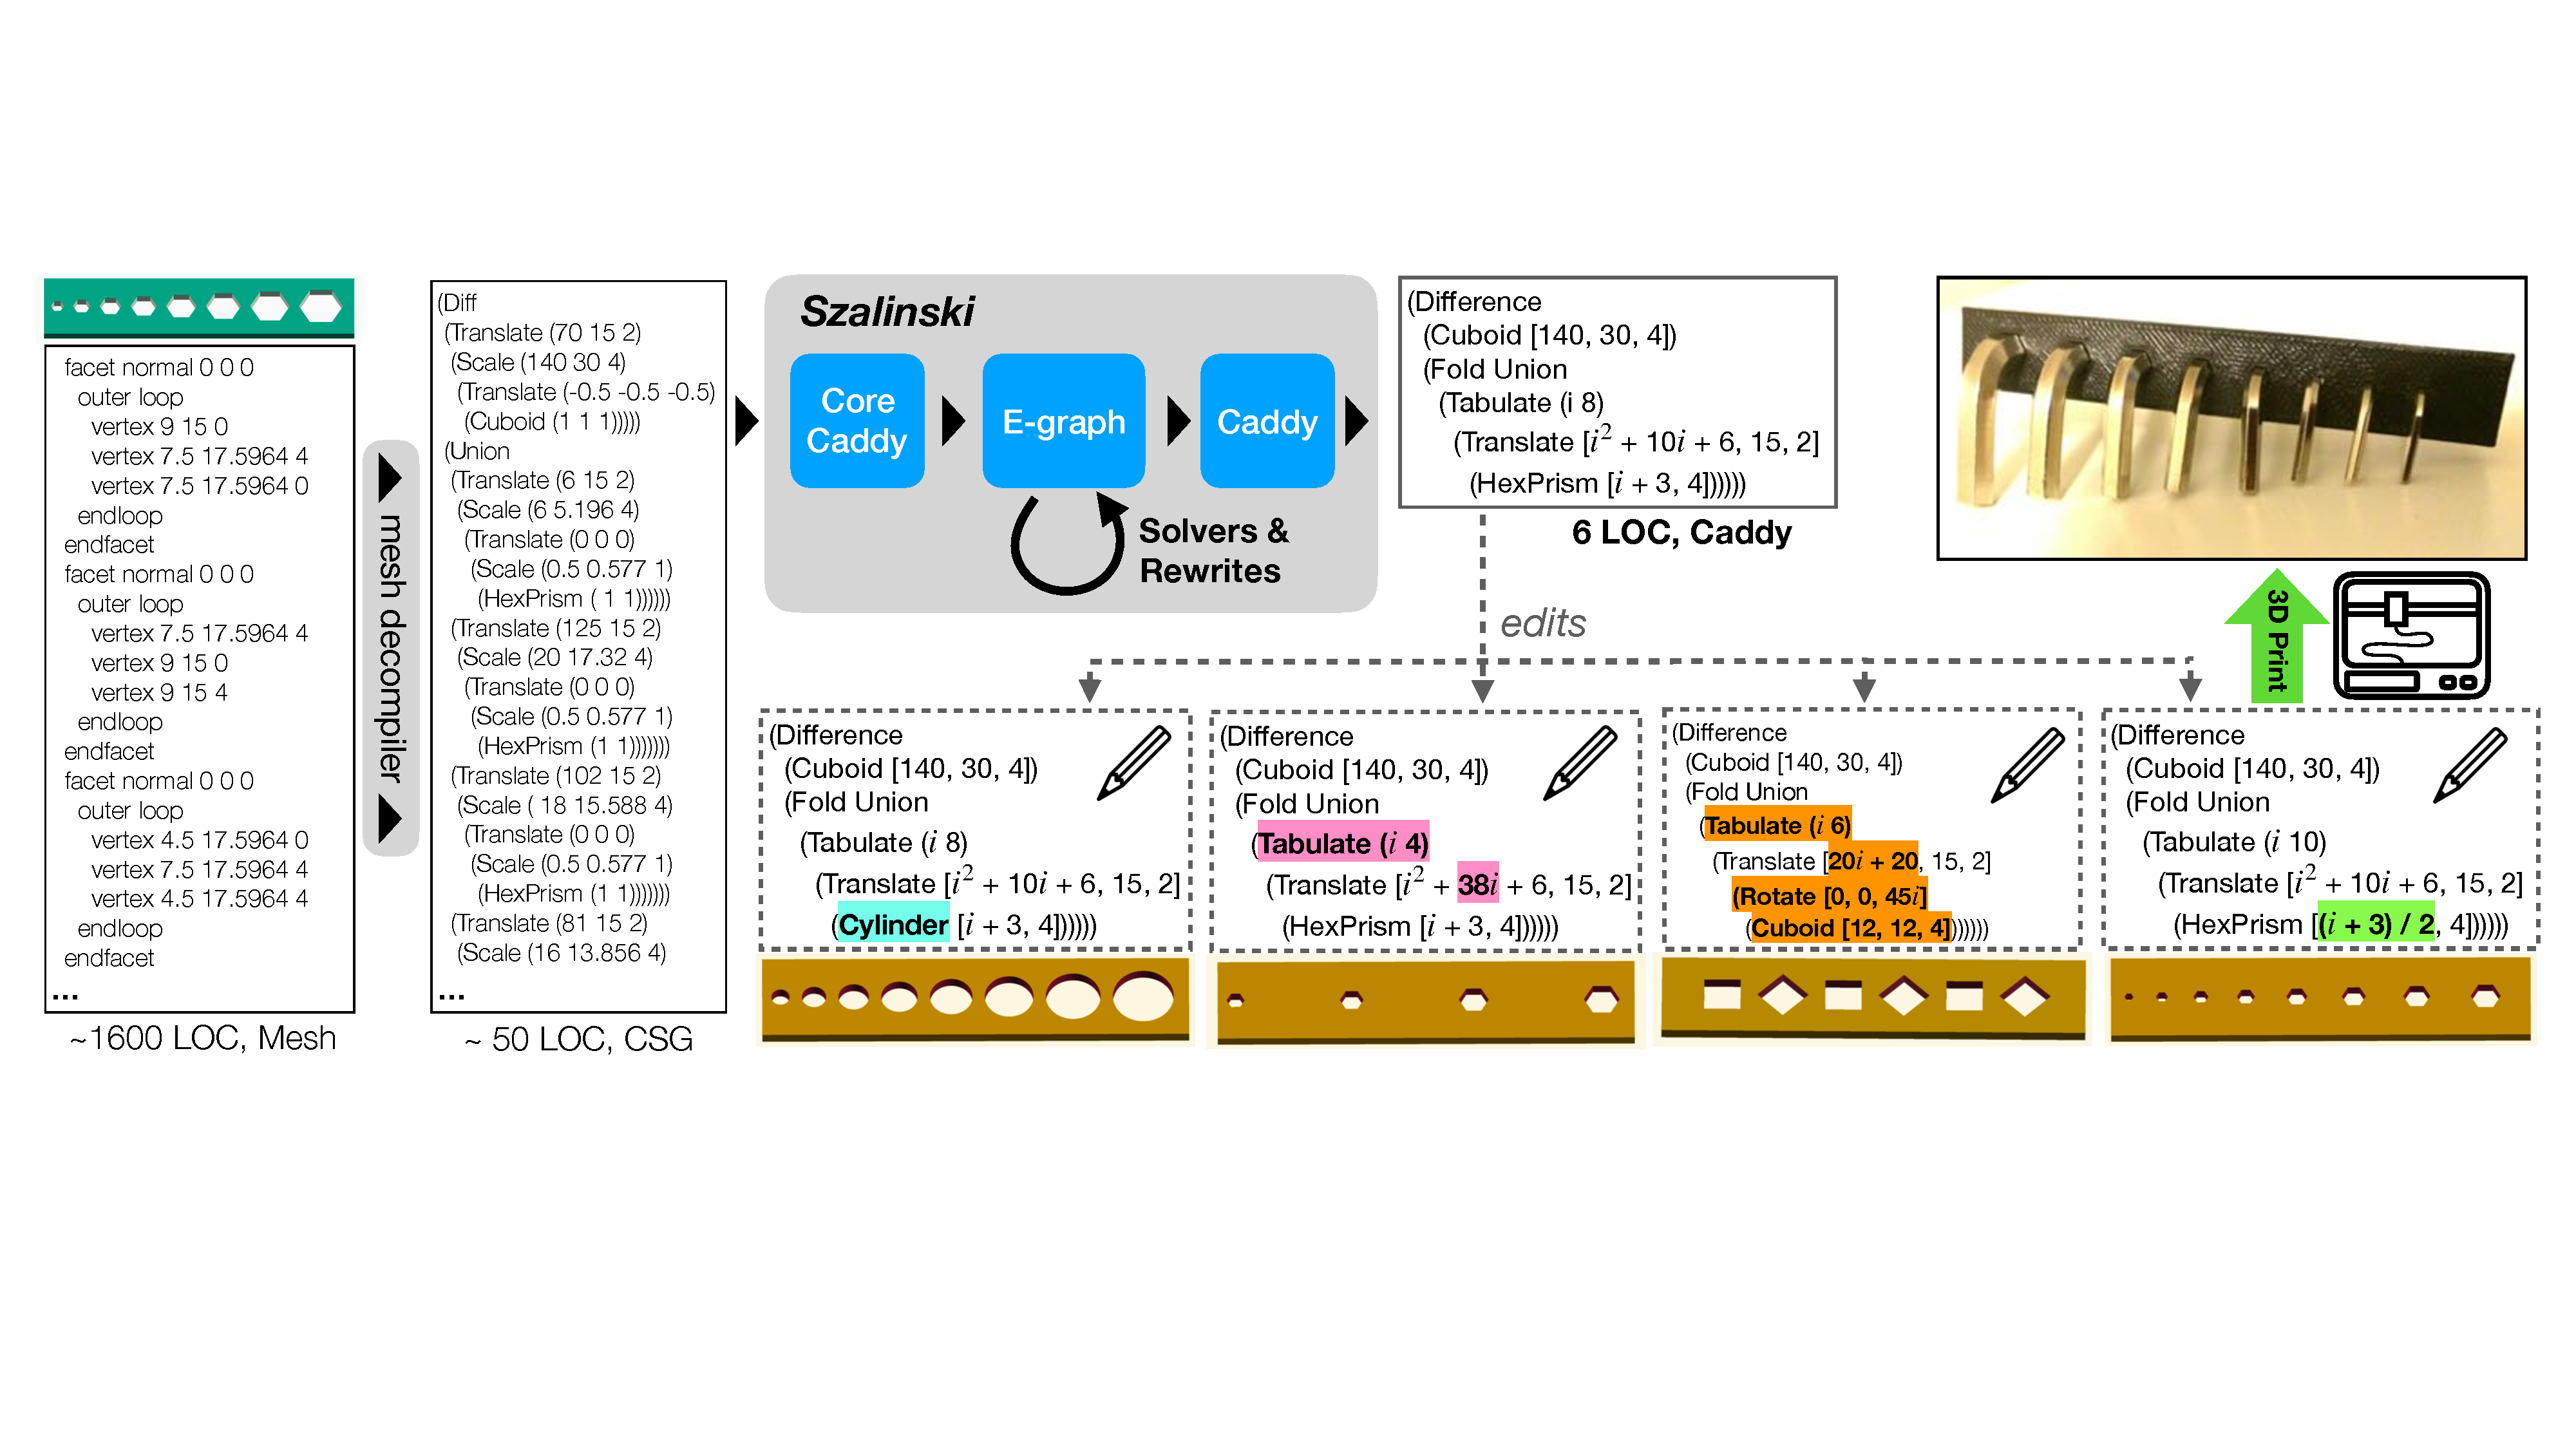
\includegraphics[width=\linewidth]{sz-overview}
  \caption[Szalinski decompiles flat CSG into structured CAD]{
  (Figure from Nandi et.\ al.\ \cite{szalinski})
  Existing mesh decompilers turn
    triangle meshes into flat, computational solid geometry (CSG) expressions.
  %  The size of both mesh and CSG are roughly proportional to
  %    the number of geometric features in the CAD model.
  \sz~\cite{szalinski} takes in these CSG expressions
    in a format called Core Caddy,
    and it synthesizes smaller, structured programs in language called Caddy
    that is enriched with functional-style features.
  This can ease customization by simplifying edits:
    small, mostly local changes
    yield usefully different models.
  The photo shows the 3D printed hex wrench holder after
    customizing hole sizes.
  \sz is powered by \egg's extensible equality saturation, relying on its high
    performance, \eclass analyses, and dynamic rewrites.
  }
  \label{fig:sz-overview}
\end{figure}

Several tools have emerged
  that reverse engineer high level
  Computer Aided Design (CAD) models from polygon
  meshes and voxels~\cite{reincarnate, inverse, shape, csgnet, latex}.
The output of these tools are constructive solid geometry (CSG) programs.
A CSG program is comprised of
  3D solids like cubes, spheres, cylinders,
  affine transformations like scale, translate, rotate
  (which take a 3D vector and a CSG expression as arguments),
  and binary operators like union, intersection, and difference
  that combine CSG expressions.
For repetitive models like a gear, CSG programs can be too long
  and therefore difficult to comprehend.
A recent tool, \sz~\cite{szalinski},
  extracts the inherent structure
  in the CSG outputs of mesh decompilation tools
  by automatically inferring maps and folds (\autoref{fig:sz-overview}).
\sz accomplished this using \egg's extensible equality saturation system,
  allowing it to:

\begin{itemize}

  \item Discover structure using loop rerolling rules.
    This allows \sz to infer functional patterns like
    \texttt{Fold}, \texttt{Map2}, \texttt{Repeat} and
    \texttt{Tabulate} from flat CSG inputs

  \item Identify equivalence among CAD terms that are
    expressed as different expressions by mesh decompilers.
    \sz accomplishes this by using CAD identities.
    An example of one such CAD identity in \sz is
    $e \leftrightarrow \mathit{rotate}~[0 ~ 0 ~ 0] ~ e$.
    This implies that any CAD expression $e$
    is equivalent to a CAD expression that applies
    a rotation by zero degrees about x, y, and z axes
    to $e$

  \item Use external solvers to
    speculatively add potentially profitable
    expressions to the \egraph.
    Mesh decompilers often generate CSG expressions
    that order and/or group list elements in
    non-intuitive ways.
    To recover structure from such expressions,
    a tool like \sz must be able to reorder and regroup
    lists that expose any latent structure

\end{itemize}

\subsection{Implementation}

Even though CAD is
  different from traditional languages
  targeted by programming language techniques,
  \egg supports \sz's CAD language in a straightforward manner.
\sz uses purely syntactic rewrites to express
  CAD identities and some loop rerolling rules
  (like inferring a \texttt{Fold} from a list of CAD expressions).
Critically, however, \sz relies on \egg's
  dynamic rewrites and \eclass analysis to infer functions
  for lists.

Consider the flat CSG program in \autoref{fig:sz-egg-input}.
A structure finding rewrite first rewrites the flat list of \texttt{Union}s to:
$$\texttt{(Fold Union (Map2 Translate [(0 0 0) (2 0 0) ...] (Repeat Cube 5)))}$$
The list of vectors is stored as \texttt{Cons} elements (sugared above for brevity).
\sz uses an \eclass analysis to track the accumulated lists in a similar style
  to constant folding.
Then, a dynamic rewrite uses an arithmetic solver to rewrite the concrete
  list of 3D vectors in the analysis data
  to \mbox{\texttt{(Tabulate (i 5) (* 2 i))}}.
A final set of syntactic rewrites can hoist the \texttt{Tabulate}, yielding the
  result on the right of \autoref{fig:sz-egg}.
Thanks to the set of syntactic CAD rewrites, this structure finding even works
  in the face of CAD identities.
For example, the original program may omit the no-op
  \texttt{Translate (0 0 0)}, even though it is necessary to see repetitive
  structure.

\begin{figure}
\begin{subfigure}[b]{0.3\linewidth}
  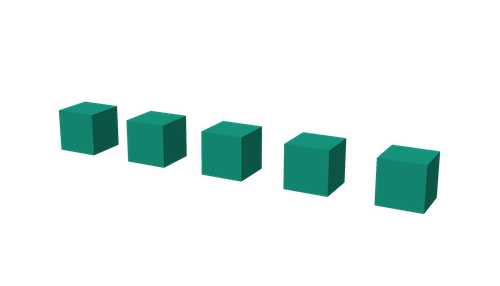
\includegraphics[width=\linewidth]{cubes}
  \caption{Five cubes in a line.}
\end{subfigure}
\hfill
\begin{subfigure}[b]{0.3\linewidth}
  \begin{lstlisting}[language=Rust, gobble=4, basicstyle=\footnotesize\ttfamily]
    (Union
      (Translate (0 0 0) Cube)
      (Translate (2 0 0) Cube)
      (Translate (4 0 0) Cube)
      (Translate (6 0 0) Cube)
      (Translate (8 0 0) Cube))
  \end{lstlisting}
  \caption{Flat CSG input to \sz.}
  \label{fig:sz-egg-input}
\end{subfigure}
\hfill
\begin{subfigure}[b]{0.35\linewidth}
  \begin{lstlisting}[language=Rust, gobble=4, basicstyle=\footnotesize\ttfamily, showlines=true, xleftmargin=5mm]
    (Fold Union
      (Tabulate (i 5)
        (Translate
          ((* 2 i) 0 0)
          Cube)))

  \end{lstlisting}
  \caption{Output captures the repetition.}
  \label{fig:sz-egg-output}
\end{subfigure}
  \caption{
    \sz integrates solvers into \egg's equality saturation as a dynamic rewrite.
    The solver-backed rewrites can transform repetitive lists into
    \texttt{Tabulate} expressions that capture the repetitive structure.
  }
  \label{fig:sz-egg}
\end{figure}

\subsection{Inverse Transformations}

In many cases, the repetitive structure of input CSG expression is further
  obfuscated because subexpressions may appear in arbitrary order.
For these inputs, the arithmetic solvers must first reorder
  the expressions to find a closed form like a \texttt{Tabulate}
  as shown in \autoref{fig:sz-egg}.
However, reordering a list does not preserve equivalence, so adding it to the
  \eclass of the concrete list would be unsound.
\sz therefore introduces \textit{inverse transformations},
  a novel technique that allows solvers to speculatively reorder and regroup list
  elements to find a closed form.
The solvers annotate the potentially profitable expression with the
  permutation or grouping that led to the successful discovery
  of the closed form.
Later in the rewriting process, syntactic rewrites eliminate the inverse
  transformations when possible
  (e.g., reordering lists under a \texttt{Fold Union} can be eliminated).
\egg supported this novel technique without modification.

\subsection{Results}
\sz's initial protoype used a custom \egraph written in OCaml.
Anecdotally, switching to \egg
  removed most of the code,
  eliminated bugs,
  facilitated the key contributions of solver-backed rewrites and inverse transformations,
  and made the tool about $1000 \times$ faster.
\egg's performance allowed a shift from running on small, hand-picked
  examples to a comprehensive evaluation on over 2000 real-world models from
  a 3D model sharing forum~\cite{szalinski}.

%%% Local Variables:
%%% TeX-master: "../thesis"
%%% End:
 \section{Herbie: Improving Floating Point Accuracy}
\label{sec:herbie}

Herbie automatically improves accuracy
  for floating-point expressions,
  using random sampling to measure error,
  a set of rewrite rules for generating program variants,
  and algorithms that prune and combine program variants
  to achieve minimal error.
Herbie received PLDI 2015's Distinguished Paper award~\cite{herbie}
  and has been continuously developed since then,
  sporting hundreds of Github stars, hundreds of downloads,
  and thousands of users on its online version.
Herbie uses \egraphs for algebraic simplification of mathematical expressions,
  which is especially important for avoiding floating-point errors
  introduced by cancellation, function inverses, and redundant computation.

Until our case study,
  Herbie used a custom \egraph implementation
  written in Racket (Herbie's implementation language)
  that closely followed traditional \egraph implementations.
With timeouts disabled,
  \egraph-based simplification consumed
  the vast majority of Herbie's run time.
As a fix, Herbie sharply limits the simplification process,
  placing a size limit on the \egraph itself and a time limit on the whole
  procedure.
When the timeout is exceeded, simplification fails altogether.
Furthermore, the Herbie authors knew of several features
  that they believed would improve Herbie's output
  but could not be implemented because
  they required more calls to simplification
  and would thus introduce unacceptable slowdowns.
Taken together, slow simplification reduced Herbie's performance, completeness,
  and efficacy.

We implemented a \egg simplification backend for Herbie.
The \egg backend is over $3000\times$ faster than Herbie's initial simplifier and
  is now used by default as of Herbie 1.4.
Herbie has also backported some of \egg's features like batch simplification and
  rebuilding to its \egraph implementation
  (which is still usable, just not the default),
  demonstrating the portability of \egg's conceptual improvements.
% This has led to over a $200\times$ speedup over its initial design,
%   demonstrating that \egg's

\subsection{Implementation}

Herbie is implemented in Racket while \egg is in Rust;
  the \egg simplification backend is thus implemented as a Rust library that
  provides a C-level API for Herbie to access via foreign-function interface (FFI).
The Rust library defines the Herbie expression grammar
  (with named constants, numeric constants, variables, and operations)
  as well as the \eclass analysis necessary to do constant folding.
The library is implemented in under 500 lines of Rust.

Herbie's set of rewrite rules is not fixed;
  users can select which rewrites to use using command-line flags.
Herbie serializes the rewrites to strings,
  and the \egg backend parses and instantiates them on the Rust side.

Herbie separates exact and inexact program constants:
  exact operations on exact constants
  (such as the addition of two rational numbers)
  are evaluated and added to the \egraph,
  while operations on inexact constants or that yield inexact outputs
  are not.
We thus split numeric constants in the Rust-side grammar
  between exact rational numbers and inexact constants,
  which are described by an opaque identifier,
  and transformed Racket-side expressions into this form
  before serializing them and passing them to the Rust driver.
To evaluate operations on exact constants,
  we used the constant folding \eclass analysis
  to track the ``exact value'' of each \eclass.%
\footnote{Herbie's rewrite rules guarantee that different exact values
  can never become equal; the semilattice \textsf{join} checks this invariant on the Rust side.}
Every time an operation \enode is added to the \egg \egraph,
  we check whether all arguments to that operation have exact value (using the analysis data),
  and if so do rational number arithmetic to evaluate it.
The \eclass analysis is cleaner than the corresponding code in Herbie's implementation,
  which is a built-in pass over the entire \egraph.

\subsection{Results}

\begin{figure}
  \centering
  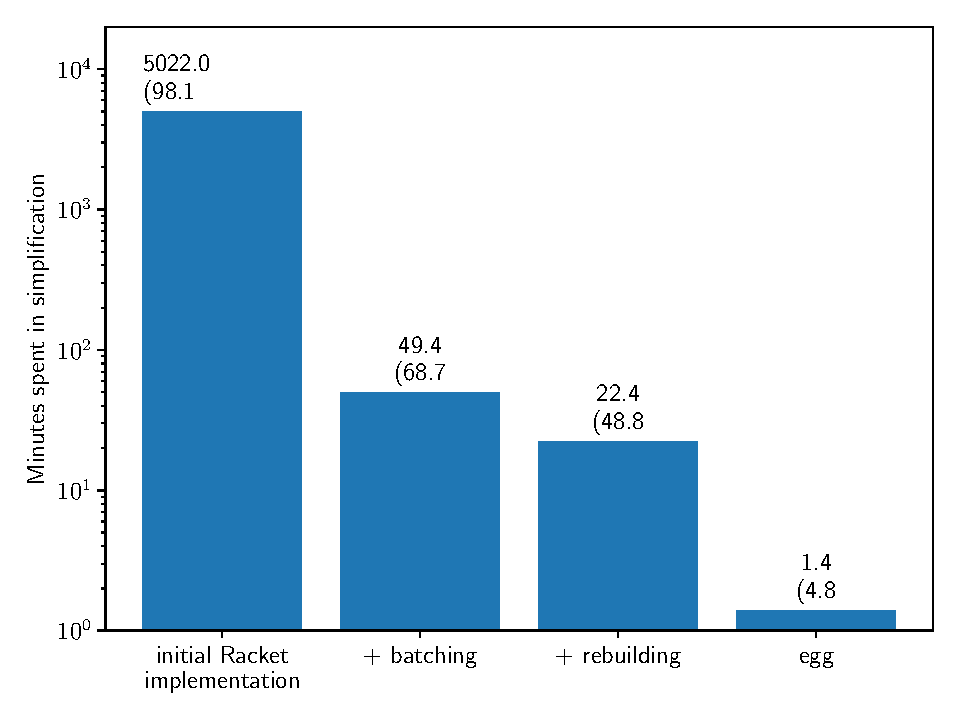
\includegraphics[height=8cm]{herbie}
  \caption{
    Herbie sped up its expression simplification phase
      by adopting \egg-inspired features like
      batched simplification and rebuilding
      into its Racket-based \egraph implementation.
    Herbie also supports using \egg itself for additional speedup.
    Note that the y-axis is log-scale.
  }
  \label{fig:herbie-results}
\end{figure}

Our \egg simplification backend
  is a drop-in replacement to the existing Herbie simplifier,
  making it easy to compare speed and results.
We compare using
  Herbie's standard test suite of roughly 500 benchmarks,
  with timeouts disabled.
\autoref{fig:herbie-results} shows the results.
The \egg simplification backend is over
  $3000\times$ faster than Herbie's initial simplifier.
This speedup eliminated Herbie's largest bottleneck:
  the initial implementation dominated Herbie's total run time at $98.1\%$,
  backporting \egg improvements into Herbie cuts
  that to about half the total run time,
  and \egg simplification takes under $5\%$ of the total run time.
Practically, the run time of Herbie's initial implementation was smaller, since
  timeouts cause tests failures when simplification takes too long.
Therefore, the speedup also improved Herbie's completeness,
  as simplification now never times out.

Since incorporating \egg into Herbie, the Herbie developers have backported some
  of \egg's key performance improvements into the Racket \egraph implementation.
First, batch simplification gives a large speedup because Herbie simplifies many
  similar expressions.
When done simultaneously in one equality saturation, the \egraph's structural
  sharing can massively deduplicate work.
Second, deferring rebuilding (as discussed in \autoref{sec:rebuilding}) gives a
  further $2.2\times$ speedup.
As demonstrated in \autoref{fig:eval-iter}, rebuilding offers an asymptotic
  speedup, so Herbie's improved implementation (and the \egg backend as well)
  will scale better as the search size grows.

%%% Local Variables:
%%% TeX-master: "../thesis"
%%% End:
 \section{Tensat: Optimizing Deep Learning Computation Graphs}
\label{sec:tensat}

\newcommand{\ourname}{Tensat}

Deep learning frameworks and compilers
 (e.g., Tensorflow~\cite{TensorFlow}, PyTorch~\cite{NEURIPS2019_9015},
  XLA~\cite{xla}, TensorRT~\cite{TensorRT}, TVM~\cite{TVM},
  MLIR~\cite{mlir})
 have enabled diverse kinds of machine learning models to run
 efficiently on numerous compute platforms.
Neural network models in
 these frameworks are typically represented as tensor computation
 graphs.
To improve the runtime performance of a tensor graph, these
 frameworks perform various optimizations.

One of the most important optimizations is graph rewriting,
 which takes in a tensor graph $g$ and a set of semantics-preserving graph rewrites $R$,
 and by applying rewrites to $g$ seeks to find an semantically equivalent $g'$ with lower cost according to some cost model.
% which transforms a tensor graph by iteratively applying rewrite rules that substitute subgraphs with semantically equivalent ones.
%The graph rewriting optimization problem can be factored into two sub-problems: (1) discovering a comprehensive set of rewrite rules and (2) an algorithm that determines the order in which to apply the rewrite rules to optimize a given graph.
The current industry-standard approach adopted by most frameworks is to use a manually curated set of rewrite rules and rely on a heuristic strategy to determine the order in which to apply the rewrite rules.
%that often applies rewrite rules greedily.
However, this approach often leads to sub-optimal results both due to the non-comprehensive set of rewrite rules, as well as the sub-optimal graph substitution heuristic \cite{taso,metaflow}. % that considers only a small fraction of all possible graphs reachable with a given set of rewrites \cite{taso, metaflow, Fang:sampling}.

This paper aims to address the sub-optimality problem of graph rewrite strategies, while leveraging the existing rewrite rules generation technique \cite{taso}.
Prior research has shown that searching for sequences of substitutions
\cite{taso,metaflow,Fang:sampling} outperforms heuristic approaches.
However, both heuristic and search-based solutions rely on sequential application of substitutions.
Since rewrites often depend on or enable one another,
optimization depends heavily on the order in which rewrites are applied;
this classically tricky problem is known in the compilers community as the ``phase-ordering'' or ``rewrite-ordering'' problem.


\begin{table}[]
    \centering
    \footnotesize
    \begin{tabular}{ccc|cc}
    \hline
    & \multicolumn{2}{c|}{\bf Search time (s)} & \multicolumn{2}{c}{\bf Runtime speedup (\%)} \\
    & TASO & \ourname{} & TASO & \ourname{} \\
    \hline
    BERT & 13.6 & \textbf{1.4} & 8.5 & \textbf{9.2} \\
    ResNeXt-50 & 25.3 & \textbf{0.7} & 5.5 & \textbf{8.8} \\
    NasNet-A & 1226 & \textbf{10.6} & 1.9 & \textbf{7.3} \\
    NasRNN & 177.3 & \textbf{0.5} & 45.4 & \textbf{68.9} \\
    Inception-v3 & 68.6 & \textbf{5.1} & 6.3 & \textbf{10.0} \\
    SqueezeNet & 16.4 & \textbf{0.3} & 6.7 & \textbf{24.5} \\
    VGG-19 & 8.9 & \textbf{0.4} & \textbf{8.9} & \textbf{8.9} \\
    \hline
    \end{tabular}
    \caption{Comparison of optimization time and runtime speedup of the optimized computation graphs over the original graphs, TASO~\cite{taso} v.s. \ourname{}.}
    \label{table:ngraph}
\end{table}


This paper presents \ourname{}, a tensor graph superoptimization framework that employs \emph{equality saturation} \cite{eqsat, eqsat-llvm, egg},
a recent technique that mitigates the phase-ordering problem by
applying all possible rewrites at once.  %comprehensively and scalably explore the search space of all equivalent graphs a given a set of rewrite rules.
Equality saturation splits program optimization into two phases: {\em exploration} and {\em extraction}.
The exploration phase uses a data structure called \emph{e-graph} to compactly generate and store all rewritings of the input program.
The exploration can continue until \emph{saturation},
where the e-graph stores all possible ways to write the input program using a given set of rewrites.
% Finally, the extraction phase selects the globally optimal equivalent program from the e-graph.
Finally, the extraction phase selects from the e-graph the equivalent program with the lowest cost according to a given cost model. The compact representation of the exponentially large search space using e-graphs enables extraction algorithms that can find the globally optimal equivalent program quickly.
%\ourname{} uses equality saturation to replace the heuristic- or sequential-search-based rewriting approaches from prior work.

% At the core of equality saturation is \emph{e-graph}: a data structure that can compactly represent equivalent expressions.
%We defer a more formal description of e-graphs to \autoref{sec:esat} and instead focus here on the intuition behind e-graphs.
%\CUT{An e-graph compactly represent a set of equivalent graphs by grouping equivalent sub-graphs into a single e-class, which is in turn used as a child node in possibly multiple sub-graphs.}
%\TODO{Remy: we need to emphasize sharing.}
% The construction of e-graphs involves repeated application of rewrite rules to add sub-graphs until \emph{saturation}, without destroying original graphs.
%\CUT{Once saturated,  any graph equivalent to the original graph under the given set of rewrite rules can then be \emph{extracted} simply by choosing one option per e-class in the saturated e-graph. }
%\TODO{Remy: this is a bit confusing, we are really picking one enode per class. Mangpo: do we need this much detail about e-graph here?}
% The graph rewriting problem can therefore be reduced to constructing a saturated e-graph for a given graph under a set of rewrite rules, and subsequently extracting the optimal graph from the e-graph .
%\CUT{by choosing a representative from each e-class}.

Applying equality saturation to tensor graph rewriting requires non-trivial extensions in both the exploration and extraction phases.
We extend the exploration phase to support complex, non-local rewrite rules that are necessary to produce highly efficient tensor graphs.
Additionally, we introduce a novel method to filter out invalid subgraphs from an e-graph,
which enables our extraction procedure based on Integer Linear Programming (ILP) to quickly find the optimal solution.

We evaluated \ourname{} on a number of well-known machine learning models executing on a GPU.
As highlighted in \autoref{table:ngraph}, \ourname{} can synthesize optimized graphs that are up to 23\% faster in runtime than state-of-the-art \cite{taso}, while reducing the optimization time by up to 300x.
By having the e-graph compactly representing an exponential number of equivalent graphs, \ourname{} is able to cover a larger search space more efficiently than the sequential search methods.
As a result, our search approach is both extremely effective and fast enough to be used as part of a normal complation flow.
%Our approach discovers better optimized graphs than the state-of-the-art, at the same time running much faster such that it can be used as part of a normal compilation flow.
%We believe that our approach is the first tensor graph superoptimization that is both \ATTN{provably optimal} and fast enough to be used as part of a normal complation flow.

%However, doing so requires non-trivial extensions in both the saturation as well as the extraction phase: (a) extending equality saturation to support complex rewrite rules (b) formulating the extraction problem as a integer linear programming(ILP), and (c) designing pruning strategies to trade-off coverage (in terms of the number of graphs explored) for shorter time to solve the ILP problem.


%We evaluated \ourname{} on a number of well-known machine learning models (including BERT, ResNeXt-50, NasNet-A, NasRNN, and Inception-v3), comparing against TASO \cite{taso}, state-of-the-art tensor graph rewriting approach.
%up to xxx faster performing graphs in up to xxx smaller search time while exploring an exponentially larger search space.
%In addition, we have also performed a number of ablation studies to highlight the importance of the specific optimizations and extensions proposed in this paper.

\subsection{Representations}

This section describes how \ourname{} represents tensor computation graphs and rewrite rules.

\subsubsection{Representing Tensor Computation Graphs}
\label{sec:language}

We use a representation based on the one in TASO \cite{taso}, with modifications to make it suitable for equality saturation.
\autoref{table:ops} shows the set of operators we consider.
Each operator $o_i$ corresponds to a node $n_i$ in the graph; the node represents the output tensor of the operator.
The nodes corresponding to the inputs of $o_i$ are the children nodes of $n_i$.
% Unlike TASO, we include both the input tensors and the operator parameters as the children nodes of the operator node.
% This way, all the relevant information of the tensor computation graph is represented syntactically by the nodes and the edges, without the need of additional annotations on the nodes.
Each tensor computation graph is a DAG under this representation.

The formulations in equality saturation becomes simpler if a graph is single-rooted. Therefore, we combine all the final output nodes of a graph with \emph{noop}s to make the graph single-rooted. The noop nodes do not have any actual operators associated with them, and they will not be altered during the exploration phase, so there is no side effects.


\begin{table}[t]
    \centering
    \label{table:ops}
    \begin{adjustbox}{width=\linewidth}
    \begin{tabular}{llll}
    \hline
        {\bf Operator}  & {\bf Description}                   & {\bf Inputs}                                                & {\bf Type signature} \\
    \hline
        ewadd           & Element-wise addition               & input$_1$, input$_2$                                        & $(T, T) \rightarrow T$ \\
        ewmul           & Element-wise multiplication         & input$_1$, input$_2$                                        & $(T, T) \rightarrow T$ \\
        matmul          & Matrix multiplication               & activation, input$_1$, input$_2$                            & $(N, T, T) \rightarrow T$ \\
        conv $^a$       & Grouped convolution                 & stride$_h$, stride$_w$, pad., act., input, weight           & $(N, N, N, N, T, T) \rightarrow T$ \\
        relu            & Relu activation                     & input                                                       & $T \rightarrow T$ \\
        tanh            & Tanh activation                     & input                                                       & $T \rightarrow T$ \\
        sigmoid         & Sigmoid activation                  & input                                                       & $T \rightarrow T$ \\
        poolmax         & Max pooling                         & {input, kernel$_{\{h,w\}}$, stride$_{\{h,w\}}$, pad., act.} & $(T, N, N, N, N, N, N) \rightarrow T$ \\
        poolavg         & Average pooling                     & {input, kernel$_{\{h,w\}}$, stride$_{\{h,w\}}$, pad., act.} & $(T, N, N, N, N, N, N) \rightarrow T$ \\
        transpose $^b$  & Transpose                           & input, permutation                                          & $(T, S) \rightarrow T$ \\
        enlarge $^c$    & Pad a convolution kernel with zeros & input, ref-input                                            & $(T, T) \rightarrow T$ \\
        concat$_n$ $^d$ & Concatenate                         & axis, input$_1$, \dots, input$_n$                           & $(N, T, \dots, T) \rightarrow T$ \\
        split $^e$      & Split a tensor into two             & axis, input                                                 & $(N, T) \rightarrow TT$ \\
        split$_0$       & Get the first output from split     & input                                                       & $TT \rightarrow T$ \\
        split$_1$       & Get the second output from split    & input                                                       & $TT \rightarrow T$ \\
        merge $^f$      & Update weight to merge grouped conv & weight, count                                               & $(T, N) \rightarrow T$ \\
        reshape $^g$    & Reshape tensor                      & input, shape                                                & $(T, S) \rightarrow T$ \\
        input           & Input tensor                        & identifier $^h$                                             & $S \rightarrow T$ \\
        weight          & Weight tensor                       & identifier $^h$                                             & $S \rightarrow T$ \\
        noop $^i$       & Combine the outputs of the graph    & input$_1$, input$_2$                                        & $(T, T) \rightarrow T$ \\
    \hline
    \end{tabular}
    \end{adjustbox}
    \caption{
        Operators supported by \ourname.
        There are four types for the nodes in our representation:
        tensor type (T), string type (S), integer type (N), and tensor tuple type (TT).
        The integer type is used to represent parameters of the
         operators, such as stride, axis, and also padding and activation modes
         (by representing different modes using different integers).
         The more complex, variable-length parameters
          (e.g. shape, axes permutation) are represented using the
          string type according to the specified formats.
          \\
    \footnotesize{$^a$ Same representation as TASO \cite{taso}. Normal and depth-wise convolutions are special cases of grouped convolutions.} \\
    \footnotesize{$^b$ Axis permutation for transpose is specified using a string with format: axis$_1$\_axis$_2$\_\dots .}\\
    \footnotesize{$^c$ Pad a convolution kernel (input) with zeros to make it the same size as ref-input. }\\
    \footnotesize{$^d$ Since each type of node needs to have a fixed number of inputs, we have a separate concat for each number of inputs. }\\
    \footnotesize{$^e$ Split the tensor in the given axis. The position of the split is at the place of the most recent concat. }\\
    \footnotesize{$^f$ Merge every \textit{count} number of groups in the grouped convolution. See TASO \cite{taso} for more details. }\\
    \footnotesize{$^g$ Specify the target shape using a string with format: dim$_1$\_dim$_2$\_\dots .}\\
    \footnotesize{$^h$ The identifier for an input or weight tensor contains its name and shape, specified as a string with format: name@dim$_1$\_dim$_2$\_\dots .}\\
    \footnotesize{$^i$ For combining the outputs of the graph to make the graph single-rooted. No actual operator is associated with noop.}
  }
\end{table}


\subsubsection{Representing Rewrite Rules}
\label{sec:rewrite}

A rewrite rule for tensor computation graph specifies that some local subgraph pattern (\textit{source pattern}) is equivalent to another subgraph pattern (\textit{target pattern}).
The input tensors to the source and target patterns are \textit{variable nodes}, which can be substituted with any concrete nodes (or e-class in equality saturation) in the current graph.
Each output tensor in the source pattern corresponds to an output tensor in the target pattern.
The two corresponding output nodes are called a pair of \textit{matched outputs}.
A rewrite rule states the equivalence between each pair of matched outputs.

We represent each source (and target) pattern using symbolic expressions (S-exprs) with variables.
Patterns with a single output is represented with an S-expr rooted on the output.
Rewrite rules with such patterns are called \textit{single-pattern rewrite rules}.
Patterns with multiple outputs are represented as a list of S-exprs rooted on each output.
Rewrite rules with multiple matched outputs are called \textit{multi-pattern rewrite rules}.
\autoref{fig:rewrite} shows an example rewrite rule and its representation.

\begin{figure}[t]
    \centering
    \includegraphics[width=\linewidth, draft=true]{figures/rewrite-example.pdf}
    \begin{scriptsize}
    Source: (matmul ?input$_1$ ?input$_2$), (matmul ?input$_1$ ?input$_3$) \\
    Target: (split$_0$ (split 1 (matmul ?input$_1$ (concat$_2$ 1 ?input$_2$ ?input$_3$)))), \\
    (split$_1$ (split 1 (matmul ?input$_1$ (concat$_2$ 1 ?input$_2$ ?input$_3$))))
    \end{scriptsize}
    \caption{
    Example rewrite rule and its representation in S-expressions.
    Identifiers starting with "?" denote variable nodes.
    For clarity, we omit the activation mode inputs to \texttt{matmul}.
    Arrows point from parent nodes to children nodes.
    1 is the axis for \texttt{split} and \texttt{concat} operators.
    % The first argument to \texttt{matmul} indicates which activation function to use.
    }
    \label{fig:rewrite}
\end{figure}

\subsection{Exploration Phase}
\label{sec:saturation}

We initialize the e-graph with the original tensor computation graph.
In each iteration of the exploration phase, we search for matches of all rewrite rules in the current e-graph, and add the target patterns and equivalence relations to the e-graph.
This process continues until either the e-graph saturates or a user-specified limit (in terms of time, e-graph size, or number of iterations) is reached.
Before applying a rewrite at a found match, we perform a \textit{shape checking} to verify if the tensor shapes in the target pattern are compatible.
This is necessary since some rewrite rules requires input tensor shapes to satisfy specific preconditions, in addition to the syntactic match.
We perform shape checking in the same way as TASO \cite{taso}.


\paragraph{Multi-Pattern Rewrite Rules}

Multi-pattern rewrite rules are an important type of rules for tensor graph superoptimization \cite{taso}.
However, most equality saturation toolkits only support efficient search methods to find matches for single-pattern rewrite rules \cite{egg, ematching}.
We introduce an algorithm for applying multi-pattern rewrites, as shown in \autoref{alg:multi}. Our algorithm leverages the existing efficient search routine for single-pattern rewrites as a subroutine.
%For clarity, we omit the handling of single-pattern rules and cycles here (those are described in \autoref{alg:cycle}).

At the beginning of the exploration phase, we collect the set of unique S-exprs present in the source patterns of the rewrite rules after canonicalization.
Here, if one S-expr can be transformed into another S-expr by variable renaming only, they will be mapped to the same canonicalized S-expr.
In each iteration of the exploration phase, we use the single-pattern search subroutine to search for matches of the canonical S-exprs.
Then for each multi-pattern rule, we take the Cartesian product of the matches found, decanonicalize the variable-to-e-class map into the original variables (using the variable renaming map stored during canonicalization), and check if the matches are compatible at the shared variables between the S-exprs (i.e., if the shared variables refer to the same e-class after the mapping).
We apply the matches that are compatible.

\begin{algorithm}[t]
\small
\caption{Applying multi-pattern rewrite rules}
\label{alg:multi}
\begin{algorithmic}[1]
\Require starting e-graph $\mathcal{G}$, set of multi-pattern rewrite rules $\mathcal{R}_m$.
\Ensure updated e-graph $\mathcal{G}$.
\State canonicalized S-expr $e_c$ = Set(\{\})
\For{rule $r \in \mathcal{R}_m$ }
\For{$i = 0, \dots, |r|-1$ } \Comment{{\scriptsize $|r|$: \#S-exprs in source pattern}}
    \State ($e$, rename\_map) = \Call{Canonical}{$r$.source[$i$]}
    \State $e_c$.insert($e$)
    \State $r$.map[i] = rename\_map
\EndFor
\EndFor

  \For{iter = 0, \dots, MAX\_ITER}
    \State $M$ = \Call{Search}{$\mathcal{G}, e_c$} \Comment{all matches for all patterns}
    \For{rule $r \in \mathcal{R}_m$ }
        \For{$i = 0, \dots, |r|-1$ }
        \State canonical matches mc$_i$ = $M$[$r$.source[i]]
        \State matches m$_i$ = \Call{Decanonical}{mc$_i$, $r$.map[$i$]}
        \EndFor
        \For{$(\sigma_0, \dots, \sigma_{|r|-1}) \in$ m$_0 \times \dots \times$ m$_{|r|-1}$}
            \If{\Call{Compatible}{$(\sigma_0, \dots, \sigma_{|r|-1})$}}
            \State \Call{Apply}{$\mathcal{G}, r, \sigma_0, \dots, \sigma_{|r|-1}$}
            \EndIf
        \EndFor
    \EndFor
  \EndFor
\State \Return $\mathcal{G}$
\end{algorithmic}
\end{algorithm}

\iffalse
\CUT{
Multi-pattern rewrite rules have some important features that require special attention.
The first one is that they can grow the e-graph infinitely.
Let's consider again the example rewrite rule in \autoref{fig:rewrite}.
This rule can be matched with any two \texttt{matmul} nodes with a shared input (input$_1$).
By applying this rule once on some match, a new \texttt{matmul} node will be created and added to the e-graph (the one on the RHS of \autoref{fig:rewrite}), which also has input$_1$ as its input.
This new \texttt{matmul} node together with any of the original \texttt{matmul} node will become a new match for this rule.
This way, the example rule can be applied infinitely to grow the e-graph.
}
\fi

In our experience, one feature of multi-pattern rules for tensor graph is that they can grow the e-graph extremely rapidly.
Let's consider again the example rewrite rule in \autoref{fig:rewrite}.
This rule can be matched with any two \texttt{matmul} nodes with a shared input (input$_1$).
By applying this rule once on some match, a new \texttt{matmul} node will be created and added to the e-graph (the one on the RHS of \autoref{fig:rewrite}), which also has input$_1$ as its input.
If the e-graph contains $N$ \texttt{matmul} nodes that has some input$_1$ at the beginning, then after iteration 1, $\mathcal{O}(N^2)$ new \texttt{matmul} nodes sharing input$_1$ will be created.
In iteration 2, each pair in these $\mathcal{O}(N^2)$ nodes will be a match, which will create $\mathcal{O}(N^4)$ new nodes.
Such double exponential growth can quickly explode the e-graph.

Based on this feature, we set a separate limit $k_{\textrm{multi}}$ on the number of iterations to apply the multi-pattern rules.
After $k_{\textrm{multi}}$ iterations, we only apply the single-pattern rules until saturation or some user-specified limit.


\subsection{Extraction Phase}

During extraction, the goal is to pick one e-node from each e-class in the e-graph to obtain an optimized graph.
The optimized graph should minimize the total cost with respect to a given cost model.
In tensor graph superoptimization, the cost model reflects the inference time taken by the graph.

\paragraph{Cost model}
We use the same cost model as TASO \cite{taso}.
Each operator has a separate and independent cost, which is the measured runtime of that operator (with the specific input sizes and parameters) on hardware.
The total cost of a graph is the sum of costs of each of its nodes.
This cost model is suitable for GPUs, since GPUs typically run one operator at a time when executing a graph.
Note that an operator can be a fused operator, consisting of multiple primitive operators, such as a fused convolution and ReLU.

\subsubsection{Extraction Algorithms}
\label{sec:extraction}

\paragraph{Greedy extraction}

We first experiment with a greedy extraction strategy that has been shown to be effective for certain domains \cite{herbie, spores, egg}.
%The first extraction method we experiment with is greedy extraction.
%It has been shown to be a simple but effective method in multiple domains \cite{herbie, spores, egg}.
For each e-class, the greedy strategy computes the total cost of the subtrees rooted on each of the e-nodes, and picks the e-node with the smallest subtree cost.

Greedy extraction is not guaranteed to extract the graph with the minimum cost, even under our independent cost model.
For example, if two children of an e-node share a subgraph, greedy extraction would ignore the sharing and overestimate the cost.

\paragraph{ILP extraction}
The second approach we experiment with is formulating the extraction problem as an Integer Linear Program (ILP).

Let $i = 0, ..., N-1$ be the set of e-nodes in the e-graph.
Let $m = 0, ..., M-1$ be the set of e-classes in the e-graph.
Let $e_m$ denote the set of e-nodes within e-class $m$: $\{i | i\in e_m \}$.
Let $h_i$ denote the set of children e-classes for e-node $i$.
Let $g(i)$ denote the e-class of e-node $i$, i.e. $i\in e_{g(i)}$.
Let $m=0$ be the root e-class.
Each e-node is associated with a cost $c_i$.

We then formulate our problem as follows:
\begin{align*}
    &\textrm{Minimize: } f(x) = \sum_{i} c_i x_i
\end{align*}
Subject to:
\begin{align}
    &x_i \in \{0, 1\}, \\
    &\sum_{i\in e_0} x_i = 1, \\
    &\forall i, \forall m \in h_i, x_i \leq \sum_{j\in e_m} x_j , \\
    & \forall i, \forall m \in h_i, t_{g(i)} - t_m - \epsilon + A (1 - x_i) \geq 0, \\
    &\forall m, 0 \leq t_m \leq 1,
\end{align}

Here we introduce a binary integer variable $x_i$ for each e-node $i$; node $i$ is selected if $x_i=1$, and not selected otherwise.
Constraint (2) ensures that one node is picked in the root e-class.
Constraint (3) ensures that if a node is picked, then at least one node in each of its children e-classes needs to be picked.
We rely on the fact that at the optimal solution, each e-class can have at most one picked node (otherwise we can remove more picked nodes in this e-class to reduce the objective while still satisfying all the constraints).
Constraints (1)--(3) and the objective encode the main extraction logic.

A more subtle requirement on the extraction phase is that the extracted graph cannot contain cycles.
While the e-graph can (and likely will) contain cycles, the extracted graph is meant to map directly to an executable tensor DAG.
The extraction procedure must therefore take care to respect the acyclic invariant of DAGs.

\autoref{fig:cycle} shows an example to illustrate how valid rewrites can produce cycles in the e-graph.
To ensure the extracted graph does not contain cycles, we introduce a real variable $t_m$ for each e-class $m$ in the ILP.
Constraint (4) ensures that the order defined by $t_m$'s is a valid topological order for the extracted graph.
Here $\epsilon < 1/M$ is a small constant for effectively encoding strict inequalities in ILP.
$A$ is a large enough constant such that $A > 1 + \epsilon$.
Constraint (5) is to limit the range for the topological order variables $t_m$'s.

We also experiment with using integer variables for $t_m$'s. In this case, $t_m$'s are constrained to take integer values between 0 to $M-1$.
Constraint (4) changes accordingly to: $\forall i, \forall m \in h_i, t_{g(i)} - t_m + A (1 - x_i) \geq 1$, where $A \geq M$.

Unlike greedy extraction, the optimal solution to the ILP is guaranteed to give a valid graph (no cycles) with the lowest cost.

% \begin{figure}
%     \centering
%     \includegraphics[width=\linewidth, draft=true]{figures/cycle.pdf}
%     \caption{Example on how a valid rewrite can introduce cycles into the e-graph. RHS is the resulting e-graph after applying the rewrite rule from \autoref{fig:rewrite} to the LHS. Dotted lines circles the e-classes. We omit the e-classes with a single node for clarity. If the node split$_1$ is picked in the right e-class, then the resulting graph will have a cycle (indicated by the red edges).}
%     \label{fig:cycle}
% \end{figure}

\subsubsection{Cycle Filtering}
\label{sec:cycle}

Similar to previous work that uses ILP extraction \cite{eqsat, spores},
we find that as the size of the e-graph grows bigger, the ILP solver takes a long time and becomes the main bottleneck.
This is mainly due to the cycle constraint (4): ILP solver struggles to find a feasible solution with these constraints.
Therefore, we explore an alternative approach by filtering cycles during the exploration phase to make sure that the e-graph does not contain any cycles at the end of the exploration phase.
This way, we can get rid of the cycle constraints in the ILP.

\paragraph{Vanilla cycle filtering}
The first method is to check if applying a substitution introduces cycles to the e-graph, and discard such a substitution.
This check is run every time before applying a substitution.
Each check requires a pass over the entire e-graph.
For one iteration during the exploration phase, if we denote $N$ as the current size of the e-graph and $n_m$ as the total number of matches of the rewrite rules on the e-graph, then this vanilla cycle filtering has complexity $\mathcal{O}(n_m N)$.

\paragraph{Efficient cycle filtering}

As the number of matches $n_m$ is typically large and scales with $N$, vanilla cycle filtering can be slow.
We therefore design a novel and more efficient cycle filtering algorithm, consisting of a \textit{pre-filtering} step and a \textit{post-processing} step.
%Intuitively, in the pre-filtering step, we run one pass over the e-graph and use the information to check a large number of substitutions.
%Then we filter the remaining cycles in a post-processing steps.
\autoref{alg:cycle} shows the pseudocode for the exploration phase with efficient cycle filtering.

At the start of each iteration, we do one pass over the e-graph to record the set of descendent e-classes for each e-node (stored in a descendants map).
During the iteration, for each match of the rewrite rules, we use the pre-stored descendants map to check if  applying a rewrite introduces cycles to the e-graph; if so, we skip this match.
Line 3--9 implements the pre-filtering step.
Notice that this check is sound but not complete: a match that passes this check can still introduce cycles to the e-graph.
This is because new descendants relations introduced by the previous rewrite in this iteration are not included in the pre-stored descendants map.

\begin{algorithm}[t]
\small
\caption{Exploration phase with efficient cycle filtering}
\label{alg:cycle}
\begin{algorithmic}[1]
\Require starting e-graph $\mathcal{G}$, set of rewrite rules $\mathcal{R}$.
\Ensure updated e-graph $\mathcal{G}$, filter list $l$
  \State $l = $ $\{\}$
  \For{iter = 0, \dots, MAX\_ITER}
    \State descendants map $d$ = \Call{GetDescendants}{$\mathcal{G}, l$}
    \State matches = \Call{Search}{$\mathcal{G}, \mathcal{R}, l$}
    \For{match $\in$ matches}
      \If{\Not \Call{WillCreateCycle}{match, $d$}}
        \State \Call{Apply}{$\mathcal{G}$, match}
      \EndIf
    \EndFor
    \While{true}
      \State cycles = \Call{DfsGetCycles}{$\mathcal{G}, l$}
      \If{len(cycles) == 0}
        \State \textbf{break}
      \EndIf
      \For{cycle $\in$ cycles}
        \State \Call{ResolveCycle}{$\mathcal{G}, l$, cycle}
      \EndFor
    \EndWhile
  \EndFor
  \State \Return $\mathcal{G}, l$
\end{algorithmic}
\end{algorithm}

To resolve the cycles we missed in the pre-filtering step, we add a post-processing step at the end of each iteration (line 10-18).
We make a pass over the e-graph in DFS order and collect a set of cycles in the e-graph.
For each cycle, we choose the last node that is added to the e-graph, and add that node to a filter list.
The nodes in the filter list are considered as removed from the e-graph.
We make sure those nodes are not picked during extraction by explicitly adding constraints $\forall i \in l, x_i = 0$ to the ILP.

By constructing a descendants map once before each iteration, each of the checking in the pre-filtering step takes constant time.
The worst case complexity of the post-processing step is $\mathcal{O}(n_c N)$, where $n_c$ is the number of cycles in the e-graph.
Since $n_c$ is typically much smaller than $n_m$, this algorithm is much faster than the vanilla cycle filtering.
In practice each DFS pass over the e-graph can find many cycles, which makes $\mathcal{O}(n_c N)$ a very conservative upper bound.

\subsection{Evaluation}

We implement \ourname{} in Rust~\cite{rust} using \texttt{egg}~\cite{egg}, an open source equality saturation library.
For the extraction phase, we use SCIP \cite{scip} as the ILP solver, wrapped by Google OR-tools \cite{ortools}.

We utilize egg's \textit{e-class analysis} feature for the shape checking discussed in \autoref{sec:saturation}.
An e-class analysis associates data with each e-class to support rewrites that are not purely syntactic.
We store all the relevant information of the tensors (shape, layout, split locations) in the analysis data and use these information for shape checking.

\subsubsection{Experimental Setup}

We compare \ourname{} with TASO \cite{taso} to evaluate our equality saturation based search.
We use the same set of rewrite rules as TASO for our experiments.
We evaluate on the inference graphs of 7 models:
\textbf{BERT} \cite{bert}, \textbf{ResNeXt-50} \cite{resnext50}, \textbf{NasNet-A} \cite{nasneta}, \textbf{NasRNN} \cite{nasrnn}, \textbf{Inception-v3} \cite{inceptionv3},
\textbf{VGG-19} \cite{vgg}, and \textbf{SqueezeNet} \cite{squeezenet}.
This benchmark set covers a wide range of commonly used state-of-the-art models, including both models for computer vision tasks and models for NLP tasks, both human-designed models and automatically-discovered models by neural architecture search.
We perform all experiments on a Google Cloud instance with one NVIDIA Tesla T4 GPU, a 16-core CPU, and 60 GB of memory.
We also experiment with ResNet-50 \cite{resnet}, but find that on T4 GPU, the rewrite rules from TASO cannot provide any speedup to the graph.

For \ourname{}, our full approach uses the efficient cycle filtering algorithm (\autoref{sec:cycle}) during the exploration phase and the ILP method without the cycle constraints (\autoref{sec:extraction}) for extraction.
We set a limit on the number of nodes in the e-graph $N_{\textrm{max}}=50000$ and the number of iterations for exploration $k_{\textrm{max}}=15$.
We terminate the exploration phase when any of the limit is reached, or the e-graph is saturated.
We set a separate limit $k_{\textrm{multi}}$ on the number of iterations to apply the multi-pattern rules.
We use a default of $k_{\textrm{multi}}=1$ for the main results in \autoref{sec:speedup} and \autoref{sec:time}, and study the effect of varying $k_{\textrm{multi}}$ in \autoref{sec:multi-vary}.
We set a timeout of 1 hour for the ILP solver.

For TASO's backtracking search, we use their default settings from their artifact evaluation code on the number of iterations\footnote{The number of iterations of the outer loop, see Algorithm 2 in \cite{taso} for more details} $n=100$ and the hyperparameter $\alpha=1.0$ for each benchmark.
We also test $\alpha=1.05$ as mentioned in their paper, and find that the difference is tiny (difference in speedup percentage is less than 0.1\% on average over the benchmarks).
Increasing to $n=1000$ leads to less than 1\% speedup gain with the cost of over 11x longer in optimization time on average.


\begin{figure}
\begin{minipage}[t]{0.48\textwidth}
    \centering
    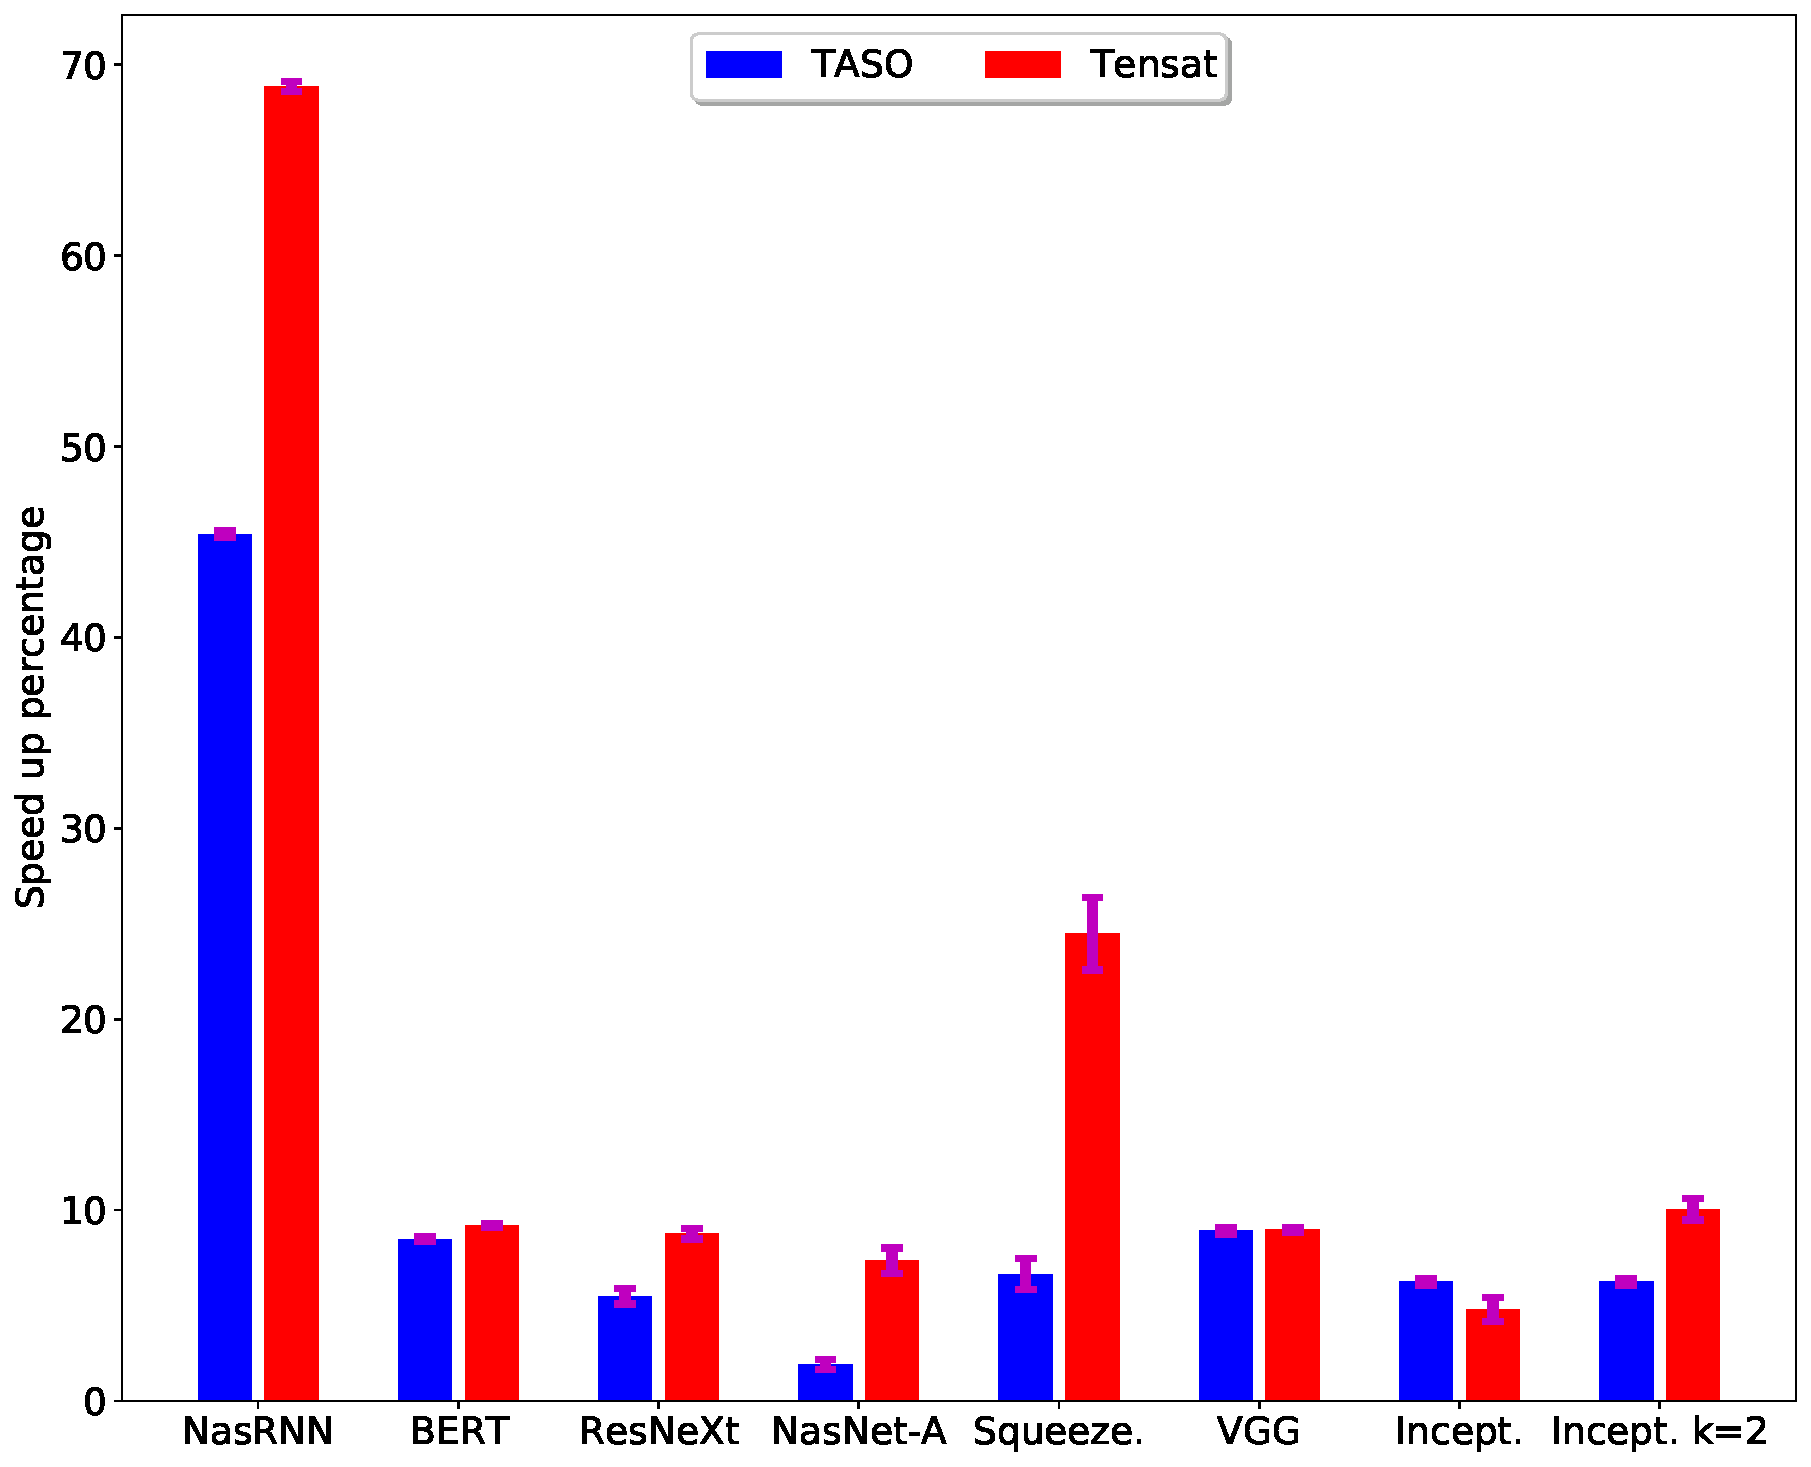
\includegraphics[width=\linewidth]{tensat/all_speedup.pdf}
    \caption{
        Speedup percentage of the optimized graph with respect to the original graph, TASO v.s. \ourname{}.
        Each setting (optimizer $\times$ benchmark) is run for five times, and we plot the mean and standard error for the measurements.
    }
    \label{fig:speedup}
\end{minipage}
\hfill
\begin{minipage}[t]{0.48\textwidth}
    \centering
    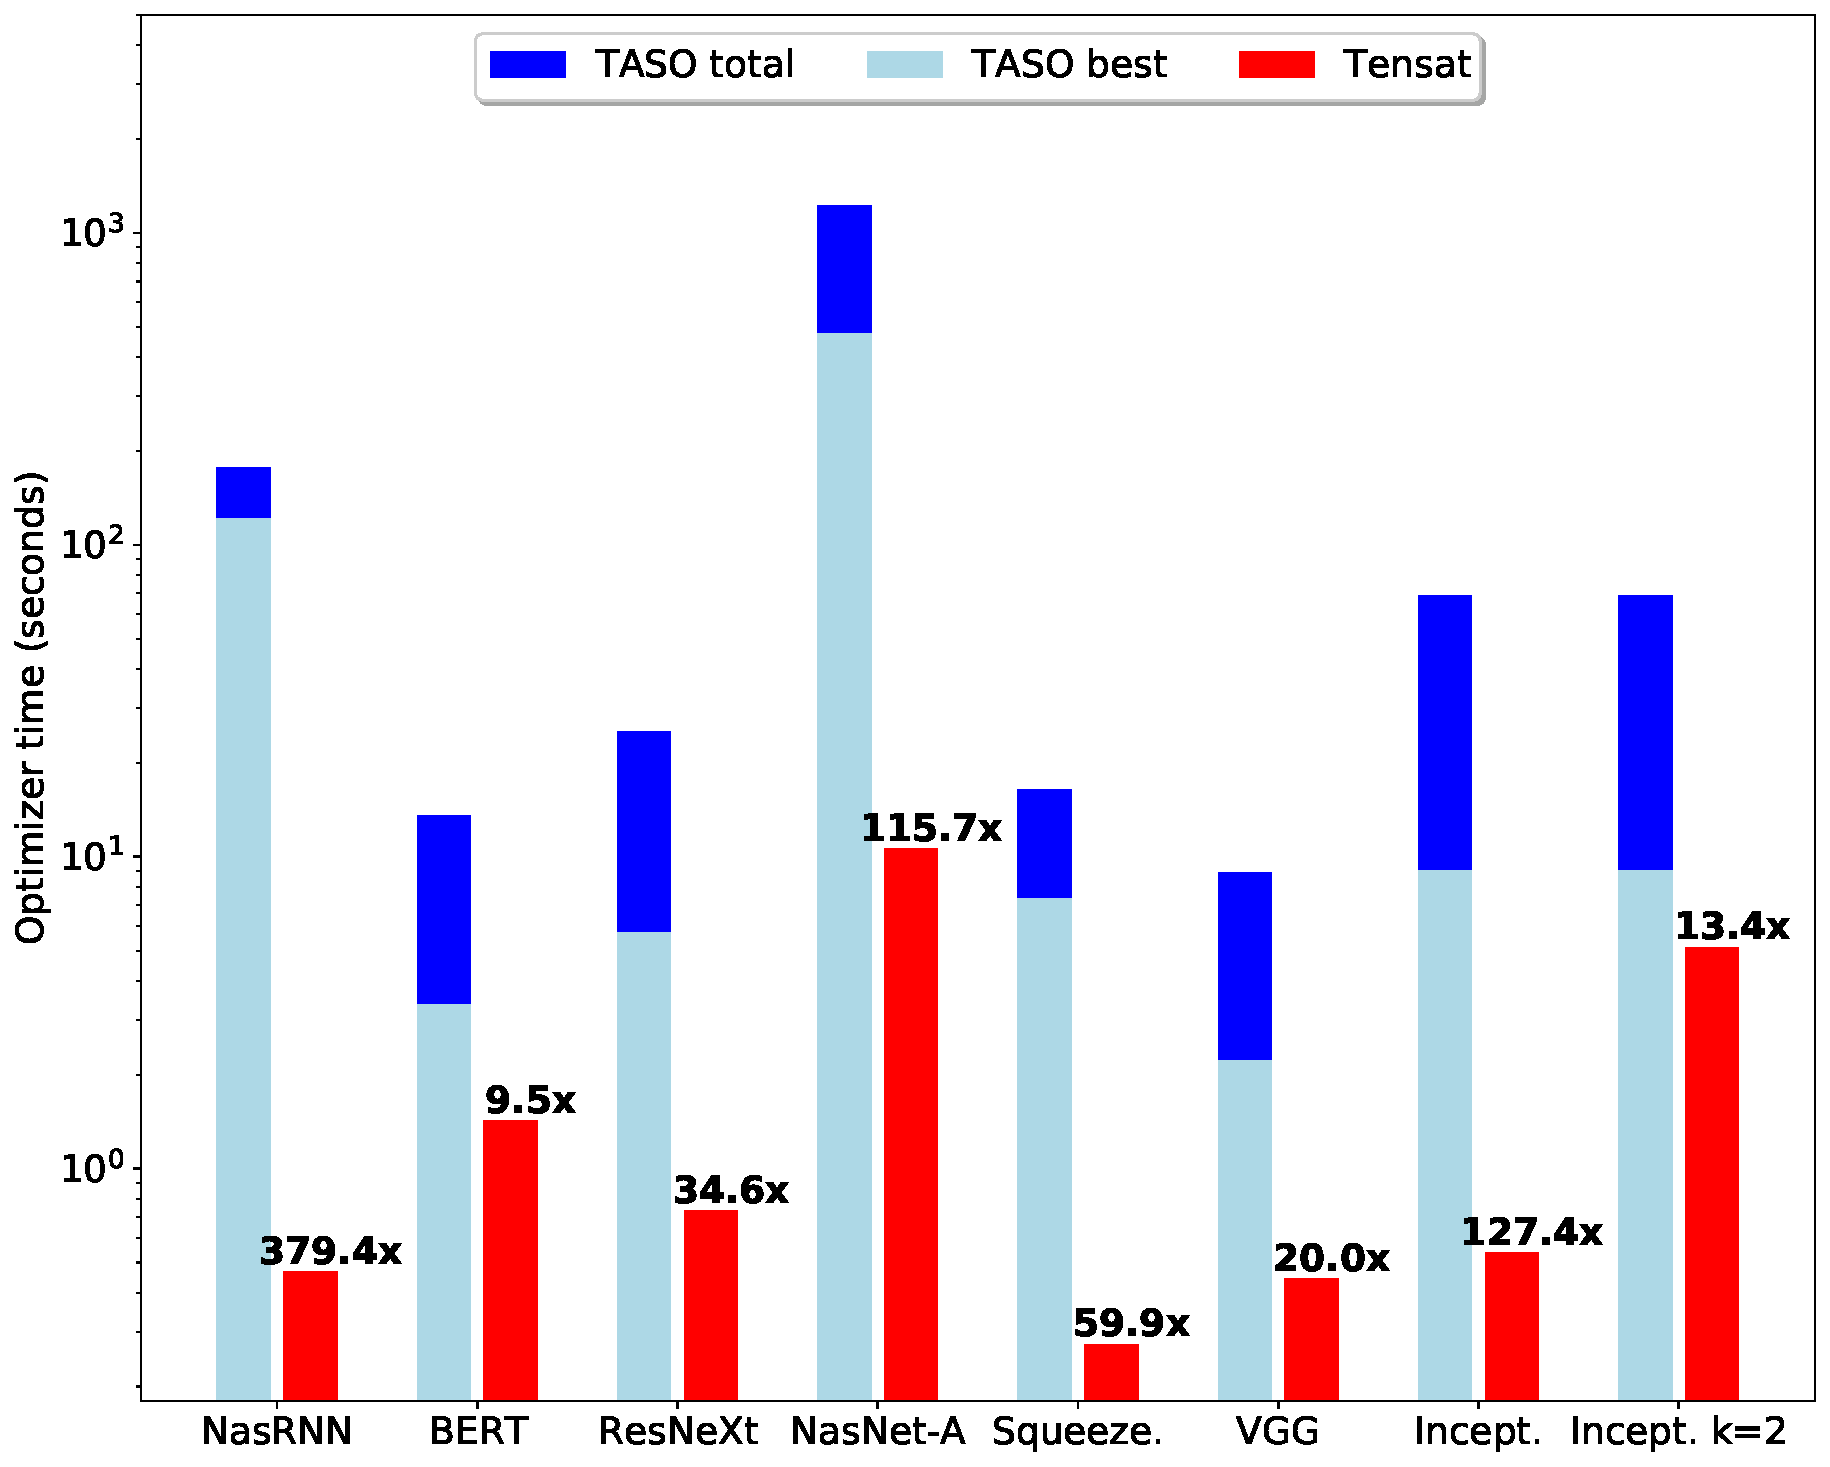
\includegraphics[width=\linewidth]{tensat/all_optim_time.pdf}
    \caption{
        Comparison of the optimization time (log scale) between TASO and \ourname{}.
        ``TASO total'' is the total time of TASO search.
        ``TASO best'' indicates when TASO found its best result;
        achieving this time would require an oracle telling it when to stop.
    }
    \label{fig:overhead}
\end{minipage}
\end{figure}

\subsubsection{Program Speedup}
\label{sec:speedup}

We compare the speedup percentage of the optimized graph with respect to the original graph between \ourname{} and TASO.
We use TASO's cuDNN backend to measure the runtime of the full computation graphs.
\autoref{fig:speedup} shows the results.
We can see that \ourname{} discovers better optimized graphs compared with TASO's backtracking search in most benchmarks.
\ourname{}'s optimized graphs are on average 6.6\% faster than TASO's. We see the biggest speedup of 23\% over TASO on NasRNN.
Note that for Inception-v3, \ourname{} with $k_{\textrm{multi}}=1$ gives a smaller speedup than TASO,
but increasing $k_{\textrm{multi}}$ to 2 achieves a better speedup than TASO
while still being 13.4$\times$ faster than TASO's search (see \autoref{fig:overhead}).

This improvement comes from the fact that equality saturation covers a much larger space of equivalent graphs than sequential backtracking search.
By using e-graph as a compact representation of an exponential number of equivalent graphs, \ourname{} is able to cover orders of magnitude more equivalent graphs than TASO.

We inspect the optimized graphs from \ourname{} and recorded some rewrite patterns that is used in them.
We present several examples of useful patterns in the Appendix.

\subsubsection{Optimization Time}
\label{sec:time}

Another important metric is the time taken by the optimizer itself.
For \ourname{}, this is the sum of time taken by the exploration phase and the extraction phase.
For TASO, we record two times for a single backtracking search.
The first is the total time of the backtracking search with the default number of iterations ($T_{\textrm{total}}$).
The second one is the time taken to first reach the best graph found during its search ($T_{\textrm{best}}$).
$T_{\textrm{best}}$ is the best possible time for TASO's sequential backtracking search.
In practice, it is difficult (if not impossible) to achieve $T_{\textrm{best}}$ since the sequential search algorithm would have no way to know that it can stop at that point.

\autoref{fig:overhead} shows the time taken by the optimizers across benchmarks.
We can see that \ourname{} runs 9.5x to 379x faster than TASO's $T_{\textrm{total}}$, and 1.8x to 260x times faster than $T_{\textrm{best}}$.
This shows that \ourname{} can not only cover a much larger search space, but also achieve this in drastically less time.
Furthermore, \ourname{}'s optimization time is small enough that we believe our approach can be integrated into a default compilation flow instead of running the search as an additional offline autotuning process.


% \subsubsection{Varying Number of Iterations for Multi-Pattern Rewrites}
% \label{sec:multi-vary}

% As we discuss in \autoref{sec:saturation}, multi-pattern rewrite rules can grow the e-graph in a extremely rapid manner.
% Here we study the effect of varying the number of iterations for multi-pattern rewrites $k_{\textrm{multi}}$.
% \autoref{fig:trend} shows the results.
% We can see the explosion of the number of nodes in the e-graph as $k_{\textrm{multi}}$ increases (due to the double exponential growth).
% For NasRNN, Inception-v3, BERT, NasNet-A, and ResNeXt-50, by increasing $k_{\textrm{multi}}$, \ourname{} discovers better graphs with larger speedups.
% But for SqueezeNet, speedup decreases with $k_{\textrm{multi}}$.
% This is due to the discrepancy between the cost model and the real graph runtime.
% As $k_{\textrm{multi}}$ increases for SqueezeNet, the cost model suggests that certain new rewrites can reduce the cost, while they in fact increase full graph runtime.
% Despite this special case where the discrepancy has an effect, \ourname{} on SqueezeNet with $k_{\textrm{multi}}=3$ still achieves a better speedup than TASO.
% By increasing $k_{\textrm{multi}}$, \ourname{} can explore a larger search space and find better optimized graphs for most benchmarks, at the cost of longer time taken by the optimizer.

% \begin{figure}
%     \centering
%     \includegraphics[width=0.29\hsize]{figures/speedup_trend.pdf}
%     \includegraphics[width=0.29\hsize]{figures/optim_trend.pdf}
%     \includegraphics[width=0.29\hsize]{figures/nodes_trend.pdf}
%     \includegraphics[width=0.09\hsize]{figures/legend_trend.pdf}
%     \caption{Effect of varying the number of iterations of multi-pattern rewrites $k_{\textrm{multi}}$.
%     For BERT, NasNet-A, NasRNN, Inception-v3, the ILP solver times out at one hour for $k_{\textrm{multi}}=3$.
%     Left: speedup of the optimized graphs (the $y$-axis is split for clarity).
%     Middle: time taken by the \ourname{}.
%     Right: final e-graph size (number of e-nodes).
%     The middle and right figures are in log scale.
%     }
%     \label{fig:trend}
% \end{figure}



\subsubsection{Ablation Study}
\label{sec:ablation}

In this section, we study the effect of the important design choices in our approach.

\paragraph{Greedy v.s. ILP extraction}

The first important design choice is the extraction method.
\autoref{table:extraction} shows the comparison between greedy extraction and ILP extraction.
Although greedy extraction works fine on some benchmarks (e.g. NasRNN), it fails to extract an optimized graph on others (e.g. BERT and NasNet-A).
This is due to the nature of greedy extraction: it makes the choices on which node to pick separately and greedily, without considering the inter-dependencies between the choices.
Consider the rewrite in \autoref{fig:rewrite} (merging two \texttt{matmul}s by \texttt{concat} and \texttt{split}) as an illustrative example.
After applying this rewrite to the e-graph, there will be two e-classes that have multiple e-nodes: one e-class per each output.
This rewrite can reduce the cost only if both e-classes choose the split node, since the RHS subgraph can be reused by the two outputs.
However, greedy extraction will never pick the split nodes, since it does not know the RHS subgraph is shared between the two split nodes.

\begin{table}[]
    \centering
    \begin{tabular}{cccc}
    \hline
        {\bf Graph Runtime (ms)} & {\bf Original} & {\bf Greedy} & {\bf ILP} \\
    \hline
        BERT & 1.88 & 1.88 & \textbf{1.73} \\
        NasRNN & 1.85 & 1.15 & \textbf{1.10} \\
        NasNet-A & 17.8 & 22.5 & \textbf{16.6} \\
    \hline
    \end{tabular}
    \caption{Comparison between greedy extraction and ILP extraction, on BERT, NasRNN, and NasNet-A.
    This table shows the runtime of the original graphs and the optimized graphs by greedy extraction and ILP extraction.
    The exploration phase is run with $k_{\textrm{multi}} = 1$. }
    \label{table:extraction}
\end{table}

\paragraph{ILP with or without cycle constraints}

Here we study the effect of whether or not to include the cycle constraints in ILP.
\autoref{table:cycle} presents the effect on extraction time as $k_{\textrm{multi}}$ (thus e-graph size) varies.
With the cycle constraints, ILP solver time quickly increases with the e-graph size, and reaches timeout when $k_{\textrm{multi}}=2$.
In our experiments, the ILP solver has not yet found a feasible solution at timeout.
Removing the cycle constraints leads to approximately 10x--1000x speedup on ILP solving time on larger e-graphs.
These results show that the main difficulty for the ILP solver is to satisfy the cycle constraints.
Thus, removing the cycle constraints makes it possible for our approach to scale to larger e-graphs.

\begin{table}[]
    \centering
    \begin{tabular}{ccccc}
    \hline
        {\bf Extraction} & \multirow{2}{*}{\bf $k_{\textrm{multi}}$} & \multicolumn{2}{c}{\bf With cycle} & {\bf Without} \\
        {\bf time (s)} & & real & int & {\bf cycle} \\
    \hline
       \multirow{2}{*}{BERT} & 1 & 0.96 & 0.98 & \textbf{0.16} \\
       & 2 & $>$3600 & $>$3600 & \textbf{510.3} \\
       \hline
       \multirow{2}{*}{NasRNN} & 1 & 1116 & 1137 & \textbf{0.32}  \\
       & 2 & $>$3600 & $>$3600 & \textbf{356.7}  \\
       \hline
       \multirow{2}{*}{NasNet-A} & 1 & 424 & 438 & \textbf{1.81}  \\
       & 2 & $>$3600 & $>$3600 & \textbf{75.1}  \\
    \hline
    \end{tabular}
    \caption{Effect of whether or not to include cycle constraints in ILP on extraction time (in seconds), on BERT, NasRNN, and NasNet-A.
    For the cycle constraints, we compare both using real variables and using integer variables for the topological order variables $t_m$. }
    \label{table:cycle}
\end{table}

\paragraph{Efficient cycle filtering}

To remove the cycle constraints from ILP, we need to perform cycle filtering during the exploration phase.
Here we compare the two cycle filtering techniques introduced in \autoref{sec:cycle}.
\autoref{table:efficient} shows the effect on the exploration phase time, as $k_{\textrm{multi}}$ varies.
We can see that the efficient cycle filtering algorithm achieves up to 2000x speedup compared with the vanilla algorithm, making it possible to explore a larger e-graph.

\begin{table}[]
    \centering
    \begin{tabular}{ccccccc}
    \hline
        \multirow{2}{*}{$k_{\textrm{multi}}$} & \multicolumn{2}{c}{BERT} & \multicolumn{2}{c}{NasRNN} & \multicolumn{2}{c}{NasNet-A} \\
        & Van. & Eff. & Van. & Eff. & Van. & Eff. \\
    \hline
        1 & 0.18 & \textbf{0.17} & 1.30 & \textbf{0.08} & 3.76 & \textbf{1.27} \\
        2 & 32.9 & \textbf{0.89} & 2932 & \textbf{1.47} & $>$3600 & \textbf{8.62} \\
    \hline
    \end{tabular}
    \caption{Comparison between vanilla cycle filtering and efficient cycle filtering, on the exploration phase time (in seconds) for BERT, NasRNN, and NasNet-A.}
    \label{table:efficient}
\end{table}


%%% Local Variables:
%%% TeX-master: "../thesis"
%%% End:
 \section{Ruler: Rewrite Synthesis using Equality Saturation}
\label{sec:ruler}

\newcommand{\rationals}{{rationals}\xspace}
\newcommand{\bfour}{{bitvector-4}\xspace}
\newcommand{\bthreetwo}{{bitvector-32}\xspace}
\newcommand{\booleans}{{booleans}\xspace}
\newcommand{\ints}{ℤ}
\newcommand{\reals}{ℝ}
\newcommand{\ruler}{Ruler\xspace}
\newcommand{\Ruler}{Ruler\xspace}
\newcommand{\cvec}{cvec\xspace}
\newcommand{\cvecs}{cvecs\xspace}


\lstdefinestyle{ruler}{
  basicstyle=\footnotesize\sffamily,
}
\lstset{
  style=ruler,
  commentstyle=\sffamily\itshape,
  columns=fullflexible,
  showstringspaces=false,
  % literate={-}{--}{1},
  % numbers=left,
  xleftmargin=0em,
  mathescape,
  language=Python,
  morekeywords={loop},
}

\begin{figure}
  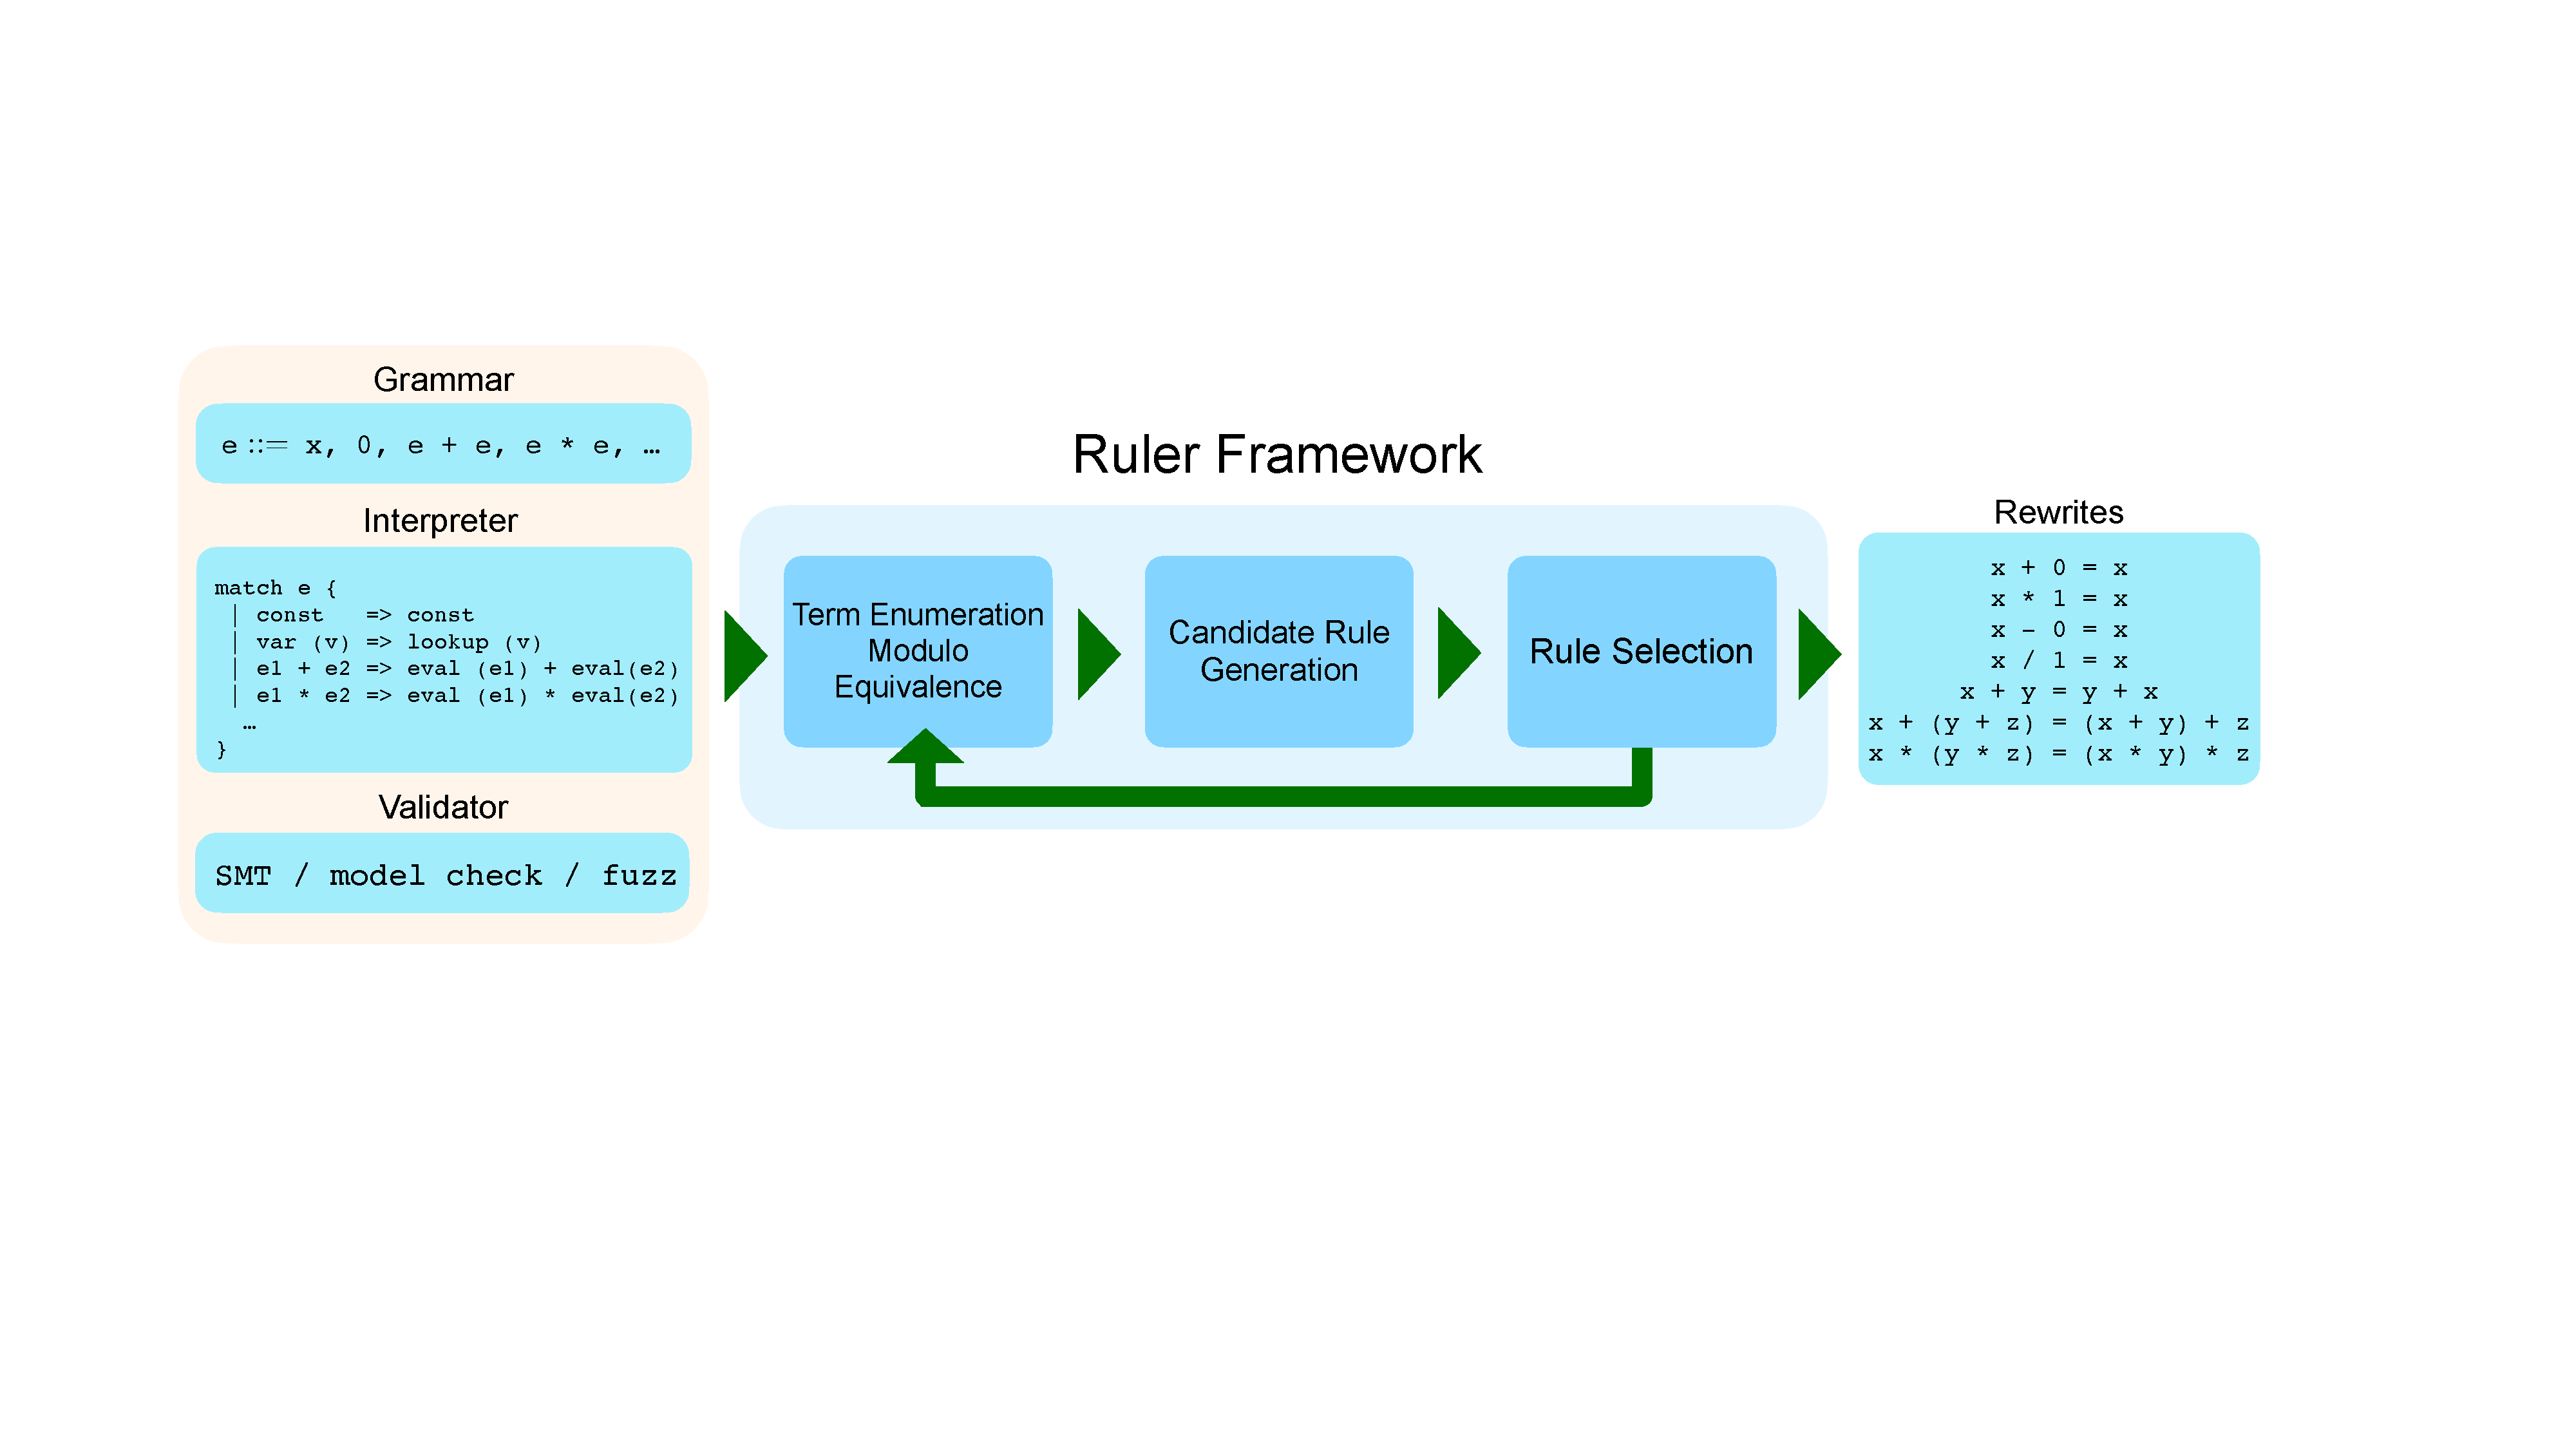
\includegraphics[width=\textwidth]{ruler-workflow.pdf}
  \caption{
    \textit{\ruler Workflow}.
    Given a grammar and interpreter for a target domain,
    \ruler uses e-graphs and equality saturation
    to efficiently enumerate potential rewrite rules and
    iteratively select a small set of general, orthogonal rules.
    \ruler supports various validation strategies to
    ensure soundness and speed up synthesis, including
    constraint solving (e.g., SMT), model checking, and fuzzing.
  }\label{fig:ruler}
\end{figure}

Many compilers, program synthesizers, and theorem provers
  rely on rewrite systems~\cite{
    haskell, arvind-hw-synth-rw, simplify}.
For example, rewriting is essential for
  improving program analyses and code generation~\cite{
    isel-survey, mlir, halide, tvm}
  and for automating verification~\cite{
    cvc4, z3, isabelle, coq}.
Without rule-based simplification,
  Halide-generated code can
  suffer $26\times$ slowdown~\cite{julie-halide}
  and
  the Herbie floating-point synthesizer~\cite{herbie}
  can return $10\times$ larger programs.

Where do the rewrite rules come from?
Several noteworthy projects have developed
  tool-specific techniques for checking or inferring rules~\cite{
    bansal, alive-infer, denali, swapper},
  but %, despite their importance,
  implementing a rewrite system
  still generally requires domain experts to
  first manually develop rulesets by trial and error.
Such slow, ad hoc, and error-prone approaches
  hinder design space exploration for new domains
  and discourage updating existing systems.


To address these challenges,
  we propose a simple, domain-general approach
  that uses \eqsat~\cite{eqsat, egg} as
  a rewrite system \textit{on the domain of rewrite rules themselves}
  to quickly synthesize effective rulesets.

In the past, tool-specific techniques
  to iteratively infer rewrite rules
  have implicitly adopted a common three-step approach,
  each constructing or maintaining a set:
\begin{enumerate}
    \item Enumerate terms from the given domain to
          build the \textit{term set} $T$.
    \item Select candidate rules from $T \times T$
          to build the \textit{candidate set} $C$.
    \item Filter $C$ to select a sound set of
          useful rules to build the \textit{rule set} $R$.
\end{enumerate}
We identify and abstract this workflow
  to provide generic rule inference for user-specified domains.

Our key insight is that \emph{what
  makes \eqsat successful in rewrite rule application
  is also useful for rule inference}.
\Eqsat can simultaneously prove many pairs of terms equivalent
 with respect to a given ruleset.
\ruler uses \eqsat to shrink
  the set $T$ of enumerated terms
  (lowering candidate \textit{generation} cost)
    by merging terms equivalent under $R$,
    and to shrink the set $C$ of candidate rules
  (lowering candidate \textit{selection} cost)
    by removing rules derivable by $R$.
Thus, \ruler uses the set $R$ of rewrite rules
  to rewrite the next batch of candidate rewrite rules
  \textit{even as $R$ is being synthesized}.


We prototyped these insights in
  a tool dubbed \ruler (\autoref{fig:ruler}).
Compared to a state-of-the-art
 rule synthesizer \cite{sat19} built
 into the CVC4 theorem prover~\cite{cvc4},
  Ruler synthesizes smaller rulesets in less time
  without reducing the set of derivable equivalences.
We demonstrate how \ruler
  can generate expert-quality rulesets
  by using it to replace all of
  Herbie's rules for rational numbers,
  uncovering missing rules that
  resolved a known bug in Herbie.

This case study's contributions include:
\begin{itemize}
  \item A novel rule synthesis algorithm
    that uses \egraphs~\cite{nelson} to
    compactly encode large sets of terms and
    \eqsat to efficiently filter and minimize rulesets
    (\autoref{sec:ruler-core}).

  \item A generic implementation of
    this algorithm within the
    \ruler
    rewrite rule inference framework
    that synthesizes rules for user-specified domains
    given a grammar and its interpreter.

  \item A comparison against a recent CVC4-based rule synthesizer
    that shows \ruler synthesizes $5.8\times$ smaller
    rulesets $25\times$ faster without compromising
    the deriving power of the rulesets.

  \item A case study demonstrating that,
    in an end-to-end application of a real world tool,
    \ruler's automatically generated rulesets
    are as good as manually-crafted expert rules
    (\autoref{sec:ruler-herbie}).

\end{itemize}

We implemented \ruler in Rust
 using \egg~\cite{egg} for
 equality saturation.
\egg's flexibility allows \ruler to be relatively simple:
 its core consists of under 1,000 lines of code,
 allowing it to be simple, extensible,
 and generic over domains.
Compared to the rewrite synthesis tool
 inside the CVC4 solver~\cite{cvc4, sat19},
 \ruler is an order of magnitude smaller.
 % Since \ruler's core algorithm does not rely on SMT,
 % \ruler can learn rewrite rules over domains
 % unsupported by SMT-LIB~\cite{smtlib},
 % or for alternative semantics for those domains
 % \footnote{For example, the Halide~\cite{halide} tool uses division semantics where $x/0=0$;
 %  this is different from the SMT-LIB semantics, but it can easily be encoded using the \texttt{ite} operator.}
 % (\autoref{subsec:updates}).

\subsection{Ruler's Algorithm}
\label{sec:ruler-core}

Like other rule synthesis approaches,
 \ruler iteratively performs three steps:
\begin{enumerate}
    \item Enumerate terms into a set $T$.
    \item Search $T \times T$ for a set of candidate equalities $C$.
    \item Choose a useful, valid subset of $C$ to add to the ruleset $R$.
\end{enumerate}

\ruler's core insight is that \egraphs and \eqsat can help
 compactly represent the sets $T$, $C$, and $R$, leading
 to a faster synthesis procedure that produces smaller
 rulesets $R$ with greater proving power.

\begin{figure}
\begin{lstlisting}[
  basicstyle=\normalsize\ttfamily,
  xleftmargin=2.5em,
  numbers=left]
def ruler (iterations):
  $T$ = empty_egraph()                            $\label{ln:empty-egraph}$
  $R$ = $\{\}$
  for $i \in [0, \texttt{iterations}]\label{ln:iterations}$:
    # add new terms directly to the e-graph representing $T$
    add_terms($T$, $i$)     $\label{ln:add-expressions}$
    loop:$\label{line:inner-loop}$
      # combine e-classes in the e-graph representing $T$ that $R$ proves equivalent
      run_rewrites($T$, $R$)    $\label{ln:run-rewrites}$
      $C$ = cvec_match($T$)             $\label{ln:cvec-match}$
      if $C = \{\}$:
        break
      # choose_eqs only returns valid candidates by using 'is_valid' internally
      $R$ = $R\ \cup$ choose_eqs($R$, $C$)                 $\label{ln:choose-eqs}$
  return $R$
\end{lstlisting}
  \caption{
  \ruler's Core Algorithm.
  The \textsf{iterations} parameter
  determines the maximum
  number of connectives in the terms
  \ruler will enumerate.
  }
  \label{fig:ruler-core}
\end{figure}

\autoref{fig:ruler-core} shows \ruler's core
  synthesis algorithm,
  which is parameterized by the following:
\begin{itemize}
    \item The number of iterations to perform the search for (line \ref{ln:iterations});

    \item The language grammar, given in the form of a term enumerator
          (\lstinline{add_terms}, line \ref{ln:add-expressions}),
          which takes the number of variables or constants to enumerate over;
\item The procedure for validating candidate rules, \lstinline{is_valid}
          (called inside \lstinline{choose_eqs}, \autoref{fig:choose-eqs} line \ref{ln:is-valid}).
\end{itemize}

These parameters provide flexibility for
 supporting different domains,
 making \ruler a rule synthesis framework
 rather than a single one-size-fits-all tool.



Ruler uses an e-graph to compactly represent the set of terms $T$.
In each iteration,
  \ruler first extends the set $T$
  with additional terms from the target language.
Each term $t \in T$ is tagged with a
 \textit{characteristic vector} (cvec) that
 stores the result of evaluating $t$ given
 many different assignments of values to variables.


After enumerating terms,
  \ruler uses \eqsat
  (\lstinline{run_rewrites})
  to  merge terms in $T$
  that can be proved equivalent
  by the rewrite rules already discovered (in the set $R$);

Next, \ruler computes a set $C$ of candidate rules (\lstinline{cvec_match}).
It finds pairs $(t_1, t_2) \in T \times T$
  where $t_1$ and $t_2$
  are from distinct \eclasses
  but have matching \cvecs
  and thus are likely to be equivalent.
Thanks to \lstinline{run_rewrites},
  no candidate in $C$ should be derivable from $R$.
However, $C$ is often still large and
  contains many redundant or invalid candidate rules.

Finally, \ruler's \lstinline{choose_eqs} procedure picks a valid subset of $C$ to add to $R$,
  ideally finding the smallest extension
  which can establish all equivalences implied by $R \cup C$.
\ruler tests candidate rules for validity using a
 domain-specific \lstinline{is_valid} function.
This process is repeated until there are no
  more equivalences to learn between terms in $T$,
  at which point \ruler begins another iteration.

% \subsection{Enumeration Modulo Equivalence}
% \label{subsec:por}

% Rewrite rules encode equivalences between terms,
%   often as relatively small ``find and replace'' patterns.
% Thus, a straightforward strategy for
%   finding candidate rules is to
%   find all equivalent pairs of terms up to some maximum size.
% Unfortunately,
%   the set of terms up to a given size grows exponentially,
%   making complete enumeration impractical for many languages.
% This challenge may be mitigated by
%   biasing enumeration towards ``interesting'' terms,
%   e.g. drawn from important workloads, or by
%   avoiding bias and using sampling techniques to
%   explore larger, more diverse terms.
% \ruler can support both
%   domain-specific prioritization and random sampling
%   via the \lstinline{add_terms} function.
% While these heuristics can be very effective,
%   they often risk missing profitable candidates
%   for new classes of inputs or use cases.


% Term space explosion can also be mitigated by
%   partitioning terms into equivalence classes
%   and only considering a single, canonical
%   representative from each class.
% Similar to partial order reduction techniques in
%   model checking~\cite{peled1998ten}
%   this can make otherwise intractable enumeration feasible.
% \ruler defaults to this complete enumeration strategy,
%   using an \egraph to compactly represent $T$ and
%   \eqsat to keep $T$ partitioned with respect to equivalences
%   derivable from the rules in $R$
%   even as they are being discovered.



% \paragraph{Enumerating Terms in an \Egraph}
% \Egraphs are designed to represent
%   large sets of terms efficiently by
%   exploiting sharing and equivalence.
% For sharing, \egraphs maintain deduplication
%   and maximal reuse of subexpressions
%   via hash-consing.
% If some term $a$ is already represented in an \egraph,
%   checking membership is constant time and
%   adding it again has no effect.
% The first time $(a + a)$ is added,
%   a new \eclass is introduced with only a single \enode,
%   representing the $+$ with
%   both operands pointing to $a$'s \eclass.
% If $((a + a) * (a + a))$ is then added,
%   a new \eclass is introduced with only a single \enode,
%   representing the $*$ with
%   both operands pointing to $(a + a)$'s \eclass.
% Thus as \ruler adds expressions to $T$,
%   only the new parts of each added expression
%   increase the size of $T$ in memory.

% On iteration $i$,
%   calling \lstinline{add_terms($T$, i)}
%   adds all (exponentially many) terms
%   with $i$ connectives to the \egraph.
% The first iteration calls \lstinline{add_terms}
%   with an empty \egraph to add terms with $i=0$ connectives,
%   thus specifying how many variables and which constants (if any)
%   will be included in the search space.
% Since these terms are added to an \egraph,
%   deduplication and sharing automatically
%   provide efficient representation,
%   but
%   they do not, by themselves,
%   provide an equivalence reduction to help avoid
%   enumerating over many equivalent terms.





% \paragraph{Compacting T using R}
% Ruler's \egraph not only stores the set of terms $T$,
%  but also an equivalence relation
%  (more specifically, a congruence relation)
%  over those terms.
% Since the children of an \enode are \eclasses,
%  a single \enode can represent
%  exponentially many equivalent terms.
% Initially, the \egraph stores no equivalences,
%  i.e., each term is in its own equivalence class.

% As the algorithm proceeds,
%  \ruler learns rules and places them in the set $R$
%  of accepted rules.\footnote{
%    While \autoref{fig:ruler-core} shows $R$ starting empty,
%    the user may instead initialize $R$ with trusted axioms if they choose.
%  }
% At the beginning of its inner loop (line \ref{ln:run-rewrites}),
%   \ruler performs \eqsat with the rules from $R$.
% Equality saturation will unify classes
%   of terms in the \egraph that can be proven
%   equivalent with rules from $R$.

% To ensure that \lstinline{run_rewrites} only
%   shrinks the term \egraph,
% \ruler performs this \eqsat
%       on a copy of the \egraph,
%       and then copies the newly learned equalities
%       back to the original \egraph.
% This avoids polluting the \egraph
%     with terms added during \eqsat.


% \ruler's inner loop only terminates
%   once there are no more rules to learn,
%   so the next iteration
%   (\lstinline{add_terms}, line \ref{ln:add-expressions})
%   \textit{only enumerates over the canonical representatives}
%   from the equivalence classes of terms with respect to $R$
%   that have been represented up to that point.
% This compaction of the term space makes
%   complete enumeration possible for non-trivial depths
%   and makes \ruler much more efficient in
%   finding a small set of powerful rules.
% \autoref{sec:ablation} demonstrates
%  how compaction of $T$ is essential to \ruler's performance.

% Since $R$ may contain rules that use partial operators,
%  \ruler's \eqsat implementation
%  only merges \eclasses whose \cvecs
%  agree in at least one non-null way
%  (see the definition of \textit{match} in \autoref{subsec:cvecmatch}).
% For example, consider that $x/x \to 1 \in R$,
%  and both $\frac{a+a}{a+a}$ and $\frac{a-a}{a-a} \in T$.
% The pattern $x/x$ matches both terms, but
%  \eqsat will not merge $\frac{a-a}{a-a}$ with $1$,
%  since $\frac{a-a}{a-a}$ is never defined.
% On the other hand,
%  $\frac{a+a}{a+a}$ can merge with $1$
%  since the \cvecs match.


% Prior work~\cite{sat19} on rule inference
%   applies multiple filtering passes to minimize rule sets
%   \textit{after} they are generated.
% These filters include
%   subsumption order,
%   variable ordering,
%   filtering modulo alpha-renaming,
%   and removing rules in the congruence closure
%   of previously found rules.
% \ruler eliminates the need for such filtering
%   using \eqsat on the \egraph representing $T$.
% Since enumeration takes place over \eclasses in $T$,
%  equivalent terms are ``pre-filtered'' automatically.

% \subsection{Candidate Rules}
% \label{subsec:cands}

% Given a set (or in \ruler's case, an \egraph) of terms $T$,
%  rewrite rule synthesis
%  searches $T \times T$ for pairs of equivalent terms that
%  could potentially be a rule to add to $R$.
% The set of candidate rules is denoted $C$.

% The naive procedure for producing candidate rules
%  simply considers every distinct pair:
%  $$C = \{ l \to r \mid l,r \in T.\ l \not= r \wedge \forall \sigma.\ l[\sigma] = r[\sigma] \}$$
% This is prohibitively expensive for two main reasons.
% First, it will produce many rules that
%  are either in or can be proven by the existing ruleset $R$.
% In fact, the naive approach should always produce
%  supersets of $C$ from previous iterations;
%  accepting a candidate rule from $C$ into $R$
%  would not prevent it from being generated in $R$ in the following iteration.
% Second, most of the candidates will be unsound,
%  and sending too many unsound candidates to \lstinline{choose_eqs}
%  burdens it unnecessarily,
%  since it must search $C$ for valid candidates by
%  invoking the user-supplied \lstinline{is_valid} procedure.
% \ruler's use of an \egraph to represent the term set $T$
%  addresses both of the these inefficiencies
%  with techniques called
%  \textit{canonical representation}
%  and
%  \textit{characteristic vectors}.

% \paragraph{Canonical Representation}
% Consider a situation where
%  $(x + y) \to (y + x) \in R$
%  and both
%  $(a + b)$ and $(b + a)$ are in $T$.
% When selecting terms from which to build a candidate rule,
%  considering both
%  $(a + b)$ and $(b + a)$
%  would be redundant;
%  any rules derived from one could be derived from the other
%  by composing it with commutativity of $+$.
% In some rewriting systems,
%  this composition of rewrites cannot be achieved
%  since cyclic rules like commutativity are not permitted.
% Equality saturation, however,
%  handles and in many cases prefers such compositional rules,
%  since it results in fewer rules to search over the \egraph.

% To prevent generating candidate rules which are already
%  derivable by the rules in $R$,
%  \ruler only considers a single term from each
%  \eclass when building candidate rules.
%  When searching for candidate rules,
%  \ruler considers only term pairs $(l, r)$
%  where $l \neq r$ and both are canonical representatives
%  of \eclasses in $T$.
% This ensures candidate rules cannot be derived from $R$;
%  if they could have been,
%  then $l$ and $r$ would have been in the same \eclass
%  after the call to \lstinline{run_rewrites}.

% \paragraph{Characteristic Vectors}
% \label{subsec:cvecmatch}

% Canonical representation reduces
%  $C$ from $T \times T$ to $T' \times T'$
%  where $T'$ is the set of canonical terms from $T$,
%  but it does not prevent a full $O(n^2)$
%  search of $T' \times T'$ for valid candidate rules.
% Ruler employs a technique called
%  \textit{characteristic vectors} (\cvecs) to
%  prevent this quadratic search by only considering
%  pairs that are \textit{likely} valid.
% Ruler associates a characteristic vector $v_i$
%  with each \eclass $i$.
% The \cvec is the result of evaluating
%  $t_i$, the canonical term in \eclass $i$,
%  over a set of inputs
%  that serves as a ``fingerprint''\footnote{
%    \autoref{sec:related}
%    discusses prior work~\cite{taso19, bansal} that uses
%    ``fingerprints" for
%    synthesizing peephole optimizations and graph
%    substitutions.}
%  for the value of that \eclass.
% Stated precisely,
%  let
%   $\sigma_j$ for $j \in [1, m]$ be a predetermined family of $m$
%   mappings from variables in $T$ to concrete values,
%   and let \textsf{eval} be the evaluator for the given language.
% The \cvec for \eclass $i$ is:
%  $$v_i = [ \textsf{eval}(\sigma_j, t_i) \mid j \in [1, m] ]$$

% \ruler computes \cvecs
%  incrementally and without redundancy during enumeration
%  using an \textit{\eclass analysis} \cite{egg}
%  to associate a \cvec with each \eclass;
%  let $i$ be an \eclass, $t_i$ its canonical term, and $v_i$ its cvec:
% \begin{itemize}
%     \item
%   when $t_i = n$ for a constant $n$,
%     $v_i$ is populated by copies of $n$;
%     \item
%   when $t_i = f(t_{j_1}, \ldots, t_{j_n})$ for some $n$-ary operator $f$ from the given language,
%     $v_i$ is computed by mapping $f$ over
%     the \cvecs of the subterms:\;
%     $v_i = \textsf{map}(f, \textsf{zip}(v_{j_1}, \ldots, v_{j_n}))$
%     \item
%   when $t_i = x$ for a variable $x$,
%     $v_i$ is populated by values from the target domain;
%   choosing values to populate the \cvecs of variables can be done randomly
%   or with a domain-specific approach
%   (\autoref{sec:ablation} compares two approaches).
% \end{itemize}

% To support partial operators (e.g., division),
%  \cvecs may have a null value in them to indicate failure to evaluate.
% We say that \cvecs \textit{match} if their
%  non-null values agree in every (and at least one) position,
%  i.e., \cvecs $ [a_1, \ldots, a_n]$ and $[b_1, \ldots, b_n]$ match iff:
% $$
%  \forall i.\ a_i = b_i \vee a_i = \textsf{null} \vee b_i = \textsf{null}
%  \quad\textrm{  and  }\quad
%  \exists i.\ a_i = b_i \wedge a_i \neq \textsf{null} \wedge b_i \neq \textsf{null}
% $$

% When \eclasses in the \egraph representing $T$ merge,
%  they will have matching \cvecs,
%  because they have been proven equivalent by valid rules.
% Ruler aborts if \cvecs of merging \eclasses do not match;
%  empirically, this helps avoid learning unsound rules
%  even when \lstinline{is_valid} is not sound (\autoref{subsec:soundness}).

% \autoref{sec:eval} and \autoref{sec:case} discuss
%   how \cvecs are generated for different domains.
% Characteristic vectors serve as a filter for validity:
%  if $i,j$ are \eclasses and $v_i$ does not match $v_j$,
%  (using the definition of match from \autoref{subsec:ruler-overview})
%  then $t_i \to t_j$ is not valid.
% This allows \ruler to not consider
%  those pairs when building $C$:
% $$ C =
% \{ t_i \to t_j \mid
%    i,j \in \text{\eclasses of $T$}.\ \textsf{match}(v_i, v_j) \}
% $$


% The
%  \lstinline{cvec_match} procedure
%  (called at \autoref{fig:ruler-core},
%   line \ref{ln:cvec-match})
%  constructs $C$ by
%  grouping \eclasses from $T$
%  based their \cvecs
%  and then taking pairs of canonical terms
%  from each of those groups.

% \paragraph{Validation}
% The candidate set $C$ contains rules that are likely,
%  but not guaranteed, to be valid.
% The \lstinline{choose_eqs} function
%  (discussed in \autoref{subsec:choose})
%  must validate these before returning them by using the
%  user-supplied \lstinline{is_valid} function.
% The soundness of \ruler's output, i.e.,
%  whether every rule in $R$ is valid,
%  depends on the soundness of the provided
%  \lstinline{validate} procedure.
% Many rule synthesis implementations \cite{swapper, taso19}
%  use SMT solvers to perform this validation.
% Ruler supports arbitrary validation procedures:
%  small domains may use model checking,
%  larger domains may use SMT,
%  and undecidable domains may decide to give up
%  a guarantee of soundness and use a sampling-based validation.
% \autoref{subsec:soundness}
%  compares validation
%  techniques for different domains.


\subsection{Choosing Rules}
\label{subsec:select}
\label{subsec:choose}

\begin{figure}
\begin{lstlisting} [
 numbers=left,
 basicstyle=\footnotesize\ttfamily,
 xleftmargin=7mm,
]
# $R$ is the accepted ruleset so far, $C$ is the candidate ruleset.
# Ruler's implementation of choose_eqs is based on a more flexible choose_eqs_n.
def choose_eqs($R$, $C$, $n = \infty\label{line:choose-eqs-n}$):
   for $\mathit{step} \in [100,\, 10,\, 1]\label{line:step}$:
       if $\mathit{step} \leq n$:
           $C$ = choose_eqs_n($R$, $C$, $n$, $\mathit{step}$)
   return $C$

# $n$ is the number of rules to choose from $C$, and $\mathit{step}$ is a granularity parameter.
# A larger $\mathit{step}$ size allows you to eliminate redundant rules faster.
def choose_eqs_n($R$, $C$, $n$, $\mathit{step}$):
   # let $K$ be the list of "keepers" which we will return
   $K = []$
   while $C \neq \emptyset\label{line:choose-eqs-loop}$:
      # pick the best $\mathit{step}$ candidate rules from $C$ according to a heuristic
      # that approximates rule "generality", including subsumption.
      $C_{\sf best},\; C$ = select($\mathit{step}$, $C$)

      # add the valid ones to $K$
      $K$ = $K \cup \{c \mid c \in C_{\sf best}.\ \texttt{is\_valid}(c) \}\label{ln:is-valid}$

      # remember all the invalid candidates in a global variable $\mathit{bad}$;
      # Ruler uses this to prevent known-invalid candidates from entering $C$ again (not shown)
      $\mathit{bad}$ = $\mathit{bad} \cup \{c \mid c \in C_{\sf best}.\ \neg\texttt{is\_valid}(c) \}$

      # stop if we have enough rules
      if $|K| \geq n$: $\label{line:stop-n}$
         return $K[0..n]$

      # try to prove terms remaining in $C$ equivalent using rules from $R \cup K$
      $C$ = shrink($R \cup K$, $C$)
   return $K$

def shrink($R$, $C\label{line:shrink}$):
   $E$ = empty_egraph()
   for $(l \to r) \in C$:
      $E$ = add_term($E$, $l$)
      $E$ = add_term($E$, $r$)
   $E$ = run_rewrites($E$, $R$)
   # return the extracted versions of rules from $C$, leaving out anything that was proven equivalent
   return $\{\texttt{extract}(E, l) \to \texttt{extract}(E, r)
            \mid  (l \to r) \in C.\;
            \neg \texttt{equiv}(E, l, r)
            \}$

\end{lstlisting}
  \caption{
    \ruler's implementation of \lstinline{choose\_eqs},
    which aims to minimize the candidate set $C$
    by eliminating subsets that the remainder can derive.
  }
  \label{fig:choose-eqs}
\end{figure}

After finding a set of candidate rules $C$,
  \ruler selects a valid subset of rules from $C$
  to add to the rule set $R$
  using the \lstinline{choose_eqs} procedure
  (\autoref{fig:ruler-core}, line \ref{ln:choose-eqs}).
As long as \lstinline{choose_eqs} returns
 a valid, non-empty subset of $C$,
 \ruler's inner loop will terminate:
 the number of \eclasses with matching \cvecs
 (i.e., the subset of $T$ used to compute $C$)
 decreases in each iteration since
 $R$ is repeatedly extended with
 rules that will cause new merges
 in \lstinline{run_rewrites}.
Ideally, \lstinline{choose_eqs}
  quickly finds a minimal extension of $R$
  that enables deriving all equivalences
  implied by $R \cup C'$ where $C'$ is
  the valid subset of $C$.


The candidate rules in $C$ are
 not derivable by $R$,
 but many of the
 candidate rules may be able to derive each other,
 especially in the context of $R$.
For example, the following candidate set
 is composed of three rules from the boolean domain,
 and any two can derive the third:

\noindent
\hfill
\lstinline{(^ x x) = false}
\hfill
\lstinline{(& x false) = false}
\hfill
\lstinline{(& x false) = (^ x x)}
\hspace{5em}


An implementation of \lstinline{choose_eqs}
 that only returns a single rule $c \in C$
 avoids this issue,
 since adding $c$ to $R$ prevents
 those rules derivable by $R \cup \{c\}$ from being
 candidates in the next iteration of the inner loop.
However,
 a single-rule implementation
 will be slow to learn rules,
 since it can only learn one at a time
 (\autoref{tab:ruler-eval} of our evaluation shows there are sometimes thousands of rules to learn).
Additionally,
 such an implementation has to decide which rule to select,
 ideally picking the ``strongest'' rules first.
For example,
 if $a,b \in C$ and $R \cup \{a\}$
 can derive $b$ but
 $R \cup \{b\}$
 can not derive $a$,
 then selecting $b$ before $a$ would be a mistake,
 causing the algorithm to incur an additional loop.


\ruler's implementation of
 \lstinline{choose_eqs}, shown in \autoref{fig:choose-eqs},
 is parameterized by a value $n$ with default of $\infty$.
At $n=1$, \lstinline{choose_eqs} simply returns a single valid candidate from $C$.
For higher $n$, \lstinline{choose_eqs}
 attempts to return a list of up to $n$ valid rules all at once.
This can speed up \ruler by requiring fewer trips around its inner loop,
 but risks returning many rules that can derive each other.
To mitigate this, \lstinline{choose_eqs} tries to not
 choose rules that can derive each other.
In its main loop (line \autoref{line:choose-eqs-loop}),
 \lstinline{choose_eqs}
 uses the \lstinline{select} function to pick the $\mathit{step}$
 best rules from $C$ according to a syntactic heuristic.\footnote{
 \Ruler's syntactic heuristic prefers candidates
  with the following characteristics (lexicographically):
 more distinct variables,
 fewer constants,
 shorter larger side (between the two terms forming the candidate),
 shorter smaller side,
 and fewer distinct operators.
}
\Ruler then validates the selected rules
 and adds them to a set $K$ of ``keeper'' rules which it will ultimately return.
It then employs the
 \lstinline{shrink} procedure (line \autoref{line:shrink})
 to eliminate candidates from $C$ that can be derived be $R \cup K$.
This works similarly to
 \lstinline{run_rewrites} in the \ruler algorithm,
 but \lstinline{shrink} works over the remaining
 \textit{candidate set} $C$ instead of the rule set $R$.

\ruler's \lstinline{choose_eqs} invokes the inner
 \lstinline{choose_eqs_n} procedure with increasing small step sizes
 ($\mathit{step}$ is defined on line \ref{line:step}).
Larger step sizes allow \lstinline{shrink} to quickly
 ``trim down'' $C$ when it contains many candidates.
However, a large step also means that
 \lstinline{choose_eqs} may admit $\mathit{step}$ rules into $K$ at once,
 some of which may be able to prove each other.
Decreasing the step size to 1 eliminates this issue.


% \ruler uses $n=\infty$ by default for maximum performance, and
%  \autoref{sec:ablation} measures the effects of this choice
%  on \ruler's performance and output.







% \subsection{Implementation}

% We implemented \ruler in Rust
%  using the \egg~\cite{egg} \egraph library for
%  equality saturation.
% By default \ruler uses Z3~\cite{z3} for SMT-based validation,
%  although using other validation backends
%  is simple (\autoref{sec:ablation}).

% \ruler's core consists of under 1,000 lines of code,
%  allowing it to be simple, extensible,
%  and generic over domains.
% Compared to the rewrite synthesis tool
%  inside the CVC4 solver~\cite{cvc4, sat19},
%  \ruler is an order of magnitude smaller.
%  Since \ruler's core algorithm does not rely on SMT,
%  \ruler can learn rewrite rules over domains
%  unsupported by SMT-LIB~\cite{smtlib},
%  or for alternative semantics for those domains
%  \footnote{For example, the Halide~\cite{halide} tool uses division semantics where $x/0=0$;
%   this is different from the SMT-LIB semantics, but it can easily be encoded using the \texttt{ite} operator.}
%  (\autoref{subsec:updates}).

% In the following sections, we provide various evaluations of
%   three representative domains on top of \ruler's core.
% Each domain highlights a
%   verification back-end, and \cvec generation strategy
%   \ruler supports:
%  \begin{itemize}
%  \item \booleans and \bfour: these are small domains which
%    \ruler can efficiently model check and generate sound rules by construction ---
%    the \cvecs are complete.
%  \item \bthreetwo: demonstrates that \ruler supports SMT-based
%    verification for large, non-uniform domains.
%  \item \rationals: demonstrates that random sampling
%    is adequate for larger but continuous domains.
%    This domain also showcases \ruler's support for partial operators like division.
%  \end{itemize}

% The implementation of booleans, bitvectors, and rationals are
%  in approximately 100, 400, and 300 lines, respectively.


\subsection{Comparison with CVC4}
\label{sec:ruler-eval}

To evaluate \ruler,
 we compared it with prior work that synthesizes rewrites using the
 CVC4 solver~\cite{sat19}.
Both Ruler and the CVC4 synthesizer
 are written in systems programming languages
 (Rust and C++, respectively),
 and both take similar approach to
 synthesizing rewrite rules:
  enumerate terms,
  find valid candidates,
  select rules and repeat.

% At the developers' suggestion,
%  we used CVC4 version 1.8
%  with
%  \textsf{--sygus-rr-synth} to synthesize rules.
% We enabled
%  their rule filtering
%  techniques
%  (\textsf{--sygus-rr-synth-filter-cong},
%  \textsf{--sygus-rr-synth-filter-match},
%  \textsf{--sygus-rr-synth-filter-order}).
% We enabled their rule checker
%  (\textsf{--sygus-rr-synth-check}) to
%  verify all synthesized rules.
%  Additionally, we also disabled use of any pre-existing rules from
%  CVC4 to guide the rule synthesis
%  (using \textsf{--no-sygus-sym-break}, \textsf{--no-sygus-sym-break-dynamic}).

% \autoref{tab:ruler-eval} shows the results of our comparison with CVC4's
%  rewrite rule synthesis.
% On average (harmonic mean),
%  \ruler produces $5.8\times$ smaller
%  rulesets $25\times$ faster than CVC4.
% Ruler and CVC4's results can derive each most of other.
% On the harder benchmarks (in terms of synthesis times),
%  \ruler's results have a higher derivability ratio;
%  they can prove more of CVC4 rules than vice-versa.


We compared \ruler against CVC4
 for \booleans, \bfour, and \bthreetwo.
% The CVC4 rewrite synthesis developers provided
%  grammars for 4-bit bitvector and boolean
%  domains,
%  so we implemented the same in \ruler.
Both \ruler and CVC4
 are parameterized by the domain
 (bool, bv4, or bv32),
 the number of distinct variables in the grammar,
 and the size of the synthesized term.\footnote{
   Size is measured in number of connectives,
   e.g., $a$ has 0, $(a + b)$ has 1,
   and $(a + (b + c))$ has 2.
   In CVC4, this is set with the
   \textsf{--sygus-abort-size} flag.
 }
All benchmarks were single-threaded
 and run on an
 AMD 3900X 3.6GHz processor with 32GB of RAM.
Both \ruler and CVC4 were given 3 variables
 and no constants to start the enumeration.

A bigger ruleset is not necessarily a better ruleset.
We designed \ruler to minimize ruleset size
 while not compromising on
 its capability to prove equalities.
We define a metric called the \textit{deriving ratio}
 to compare two rulesets.
Ruleset $A$ has deriving ratio $p$ with respect to ruleset $B$
 if set $A$ can derive a fraction $p$ of the rules in $B$
 ($A \vDash b$ means rule set $A$ can prove rule $b$):
$$p = |B_A| / |B| \quad\textrm{ where }\quad B_A = \{b \mid b \in B.\ A \vDash b\}$$
% in other words,
%  we find $B_A \subseteq B$ such that
%  $\forall b  \in B_A, A \vDash b$
%  and
%  $\forall b \in B \setminus B_A, A \not\vDash b$ and then compute $p = |B_A|/|B|$.
If $A$ and $B$ have deriving ratio of 1 with respect to each other,
  then they can each derive all of the other's rules.

We use \egg's equality saturation procedure to test derivability.
To test whether $A \vDash b$ (where $b = b_l \to b_r$)
 we add $b_l$ and $b_r$ to an empty \egraph,
 run \eqsat using $A$,
 and check to see if the \eclasses of $b_l$ and $b_r$
 merged.
We run \egg with 5 iterations of equality saturation.
Since this style of proof is bidirectional
 (\egg is trying to rewrite both sides at the same time),
 derivations of $b_l = b_r$ can be as long as 10
 rules from $A$.

\begin{table}
  \centering
  \begin{tabular}{lr|rrl|rrl|rr}
        \multicolumn{2}{c}{Parameters} &
        \multicolumn{3}{c}{Ruler} &
        \multicolumn{3}{c}{CVC4} &
        \multicolumn{2}{c}{Ruler / CVC4}
        \\
        Domain & \# Conn &
        Time (s) & \# Rules & Drv &
        Time (s) & \# Rules & Drv &
        Time & Rules
        \\
        \hline
bool & 2 & 0.01 & 20 & 1 & 0.13 & 53 & 1 & 0.06 & 0.38\\
bool & 3 & 0.06 & 28 & 1 & 0.82 & 293 & 1 & 0.07 & 0.10\\
bv4  & 2 & 0.14 & 49 & 1 & 4.47 & 135 & 0.98 & 0.03 & 0.36\\
bv4  & 3 & 4.30 & 272 & 1 & 372.26 & 1978 & 1 & 0.01 & 0.14\\
bv32 & 2 & 13.00 & 46 & 0.97 & 18.53 & 126 & 0.93 & 0.70 & 0.37\\
bv32 & 3 & 630.09 & 188 & 0.98 & 1199.53 & 1782 & 0.91 & 0.53 & 0.11\\
\hline
\multicolumn{8}{r|}{} & 0.04 & 0.17 \\
\multicolumn{8}{r}{} & \multicolumn{2}{r}{Harmonic Mean}
    \end{tabular}
    \vspace{1em}
  \caption{
    \ruler tends to synthesize smaller, more powerful rulesets in less
     time than CVC4.
    The table shows synthesis results
     across domains,
     and number of variables in the grammar,
     and maximum term size (in number of connectives, ``\# Conn'').
    The domains are \booleans, \bfour, and \bthreetwo.
    For verification, \ruler uses model checking for \booleans and \bfour
     and Z3 for \bthreetwo.
    The ``Drv'' column shows the fraction
     that tool's synthesized ruleset can derive of the other's ruleset;
     for example, the final row indicates that
     \ruler's 188 rules derived 98\% of CVC4's 1,782 rules,
     and CVC's rules derived 91\% of \ruler's.
    The final two columns show the ratios of
     synthesis times and ruleset sizes between the two tools.
  }
  \label{tab:ruler-eval}
\end{table}

\autoref{tab:ruler-eval} shows the results of our comparison with CVC4's
 rewrite rule synthesis.
On average (harmonic mean),
 \ruler produces $5.8\times$ smaller
 rulesets $25\times$ faster than CVC4.
Ruler and CVC4's results can derive each most of other.
On the harder benchmarks (in terms of synthesis times),
 \ruler's results have a higher derivability ratio;
 they can prove more of CVC4 rules than vice-versa.


\subsection{Synthesizing Herbie Rewrites}
\label{sec:ruler-herbie}

We also demonstrate that \ruler-generated rules
 can replace and augment those generated by experts
 by doing exactly that for the Herbie tool~\cite{herbie}
 (described in \autoref{sec:herbie}).

\paragraph{Experimental Setup}

We implemented rational numbers in \ruler,
  synthesized rewrite rules
  over rational arithmetic,
  and then ran Herbie
  with the resulting ruleset.

The Herbie benchmark suite has 51 stable benchmarks
 that contain only rational operators
 (as opposed to things like \texttt{sin} and \texttt{cos}).
We ran Herbie on these benchmarks under four different configurations:
\begin{itemize}
\item \lstinline{None}: remove all the
  rational rewrite rules from Herbie's simplification phase.
Rational rules are those which consist only of rational operators
  and no others.
Note that all other components of Herbie are left intact,
  including rules over
  rational operators combined with other operators,
  and rules entirely over
  other operators.
\lstinline{None} is the baseline.
\item \lstinline{Herbie}: no changes to Herbie, simply run it on the 51 benchmarks.
\item \lstinline{Ruler}: replace Herbie's rational rules with output of \ruler.
\item \lstinline{Both}: run Herbie with both \ruler's rational rules and the
  original Herbie rational rules.
  \end{itemize}

We used \ruler to synthesize rational rules of depth 2 with 3 variables.\footnote{
  For rationals, the \lstinline{add_terms} implementation enumerates terms by depth rather
  than number connectives, since that matches the structure of Herbie's
  existing rules.
}
\ruler learned 50 rules in 18 seconds, all of which were proven sound with an SMT post-pass.
Four rules were expansive --- i.e., rules like $( a \to (a \times 1) )$ whose LHS is only a variable.
We removed these expansive rules from the ruleset as per the recommendation of
  the Herbie developers.
% Herbie's rules are uni-directional --- we therefore expanded our
%  rules for compatibility, ultimately leading to 76 uni-directional
%  \ruler rules.
% \todo{our rules are bidirectional should we say?
% say that we expand to make them unidirectional.
% }

\begin{figure}
\begin{subfigure}[t]{0.3\linewidth}
   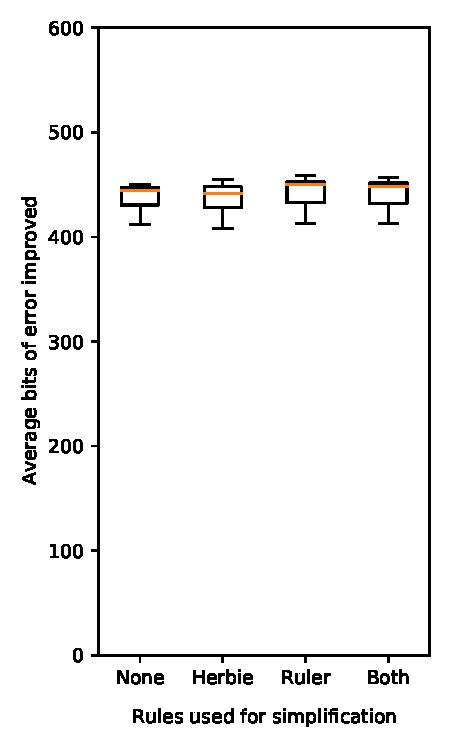
\includegraphics[width=\linewidth]{herbie-ruler/default-error.pdf}
   \caption{
     Improvement in average error,
     Herbie's metric for measuring accuracy
     (higher is better).
    }
\end{subfigure}
\hfill
\begin{subfigure}[t]{0.3\linewidth}
   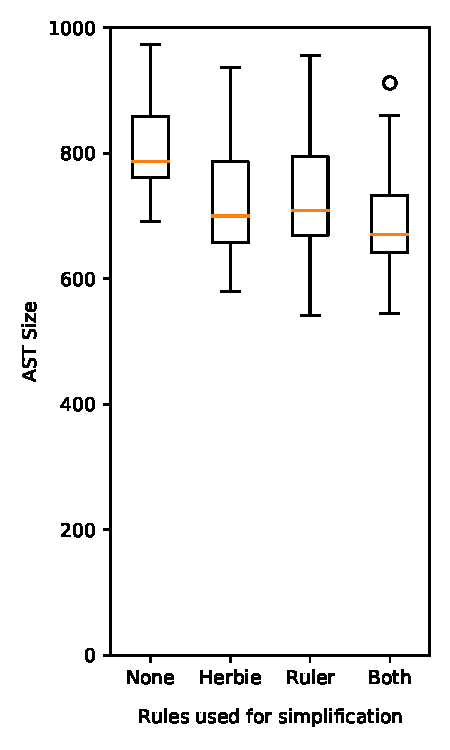
\includegraphics[width=\linewidth]{herbie-ruler/default-ast.pdf}
   \caption{
     Size of the output AST produced by Herbie
     (lower is better).
   }
\end{subfigure}
\hfill
\begin{subfigure}[t]{0.3\linewidth}
  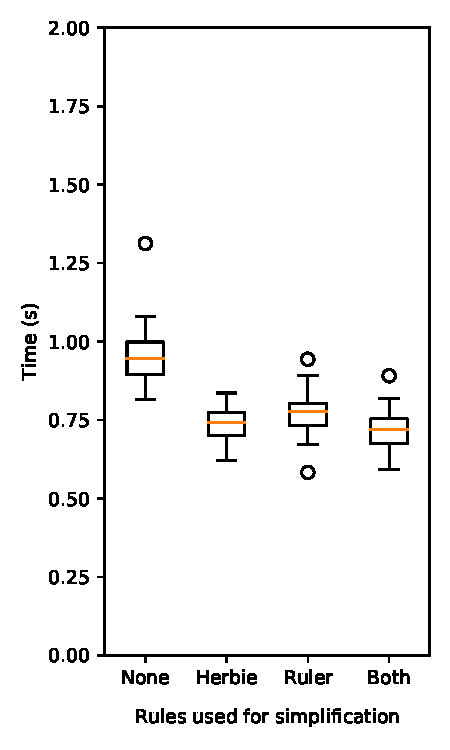
\includegraphics[width=\linewidth]{herbie-ruler/default-time.pdf}
  \caption{
  Herbie's running time (lower is better).
  }
\end{subfigure}
\caption{
 Comparing Herbie results between four configurations.
Each boxplot represents the results from 30 seeds,
 where each data point is obtained by summing the value
 (average error, AST size, time) over all 51 benchmarks.
The columns dictate what rational rules Herbie has access to:
 either none, its default rules, only \ruler's rules, or both.
Herbie's rational rules reduce AST size
 and speed up simplification without reducing accuracy,
 and \ruler's rules perform similarly (with or without Herbie's rules).
}
\label{fig:ruler-herbie}
\end{figure}

\paragraph{Discussion}
The Herbie simplifier uses equality saturation
  to find smaller, equivalent programs.
The simplifier itself does not directly improve accuracy;
  rather, it generates more candidates that are then used in the other
  accuracy improving components of Herbie.
While ideally, Herbie would return a more accurate \textit{and} smaller
 output, Herbie's ultimate goal is to find more accurate expressions,
  even if it sacrifices AST size.
Herbie's original ruleset has been developed
  over the past 6 years by
  numerical methods experts to effectively
  accomplish this goal.
%   and is often updated to include
%   custom rewrites directed towards
%   improving the accuracy specific benchmarks.
Any
  change to these rules
%   automated tool for synthesizing rewrite rules for Herbie,
  must therefore ensure that it does not make
  Herbie's result less accurate.
%   than
%   Herbie's original rewrite rules.
  %in order to be useful and practical for Herbie.

\autoref{fig:ruler-herbie} shows the results of running Herbie
  with rules synthesized by \ruler.
Each box-plot corresponds to one of the four configurations.
The baseline (\lstinline{None}) and
   \lstinline{Herbie}
  in \autoref{fig:ruler-herbie}'s
  accuracy and AST size plots highlight the significance of
  rational rewrites in Herbie ---
  these expert-written rules
  reduce AST size without
  reducing accuracy.
The plots for \lstinline{Ruler}
  show that running Herbie with only \ruler's rational rules
   has almost the same effect on accuracy and AST size
   as Herbie's original, expert written ruleset.
The plot for \lstinline{Both} shows that running Herbie together
  with Ruler's rules further reduces AST size,
  still without affecting accuracy.
The timing plots show that adding \ruler's rules to Herbie
  does not make it slower.
The baseline timing is slower than the rest because
  removing all rational
  simplification rules causes Herbie's other components
  take much longer to find the same results.\\

In summary, \ruler's rational rewrite rules can be easily integrated
  into Herbie, and they perform as
  well as expert-written rules without incurring any additional
  overhead.

% \paragraph{Derivability} Herbie's original rational ruleset consisted of
%   52 rational rules.
% \ruler synthesized 76 uni-directional rational rules (50 bidirectional rules).
% We compared the two rulesets for proving power, by deriving
%   each with the other using the approach described in \autoref{subsubsec:derive}.
% We found that Herbie's ruleset was able to
%   derive 42 out of the 50 \ruler rules.
% It failed to derive the remaining 8.
% \ruler on the other hand, was able to derive all 52 rules from Herbie.
% We highlight two of the 8 \ruler rules that Herbie's ruleset failed to derive
% that concern multiplications interaction with absolute value:
% $(|a \times b| \to |a| \times |b|)$, and
% $(|a \times a| \to a \times a)$.

\paragraph{Fixing a Herbie Bug}

\ruler
 found the following two rules that
 helped the Herbie team address a GitHub issue~\cite{herbie-bug}:
$(|a \times b| \to |a| \times |b|)$, and
$(|a \times a| \to a \times a)$.
In many cases, Herbie may generate large,
 complex outputs without improving accuracy, which makes
 the program unreadable and hard to debug.
This is often due to lack of appropriate rules for
  expression simplification.
The issue raised by a user (\cite{herbie-bug}) was in fact due to the
 missing rule $(|x| \times |x| \to x \times x)$.
The two rules above, can together, accomplish the effect of this
 rule, thereby solving the issue.
We submitted these two rules to the Herbie developers and they
 added them to their ruleset.


%%% Local Variables:
%%% TeX-master: "../thesis"
%%% End:
\chapter{Conclusion}
\label{sec:conclusion}

\Thesisstmt

\cite{Cheli2021}


%%% Local Variables:
%%% TeX-master: "../thesis"
%%% End:

\clearpage
\addcontentsline{toc}{chapter}{Bibliography}
\singlespacing
\bibliographystyle{alpha}
\bibliography{references}

\end{document}
